% for section-numbered lemmas etc., use "numberwithinsect"
\documentclass[a4paper,english,numberwithinsect]{eurocg26}

% the recommended bibstyle
\bibliographystyle{plainurl}

% -------------------------------------------------------------------
\usepackage{microtype} % if unwanted, comment out

%helpful if your graphic files are in another directory
\graphicspath{{./figures/}}

\usepackage[LGR, T1]{fontenc}
\usepackage[utf8]{inputenc}
\usepackage{lmodern, amsmath}
\newcommand\capAlpha{\mathord{\text{%
\fontencoding{LGR}\upshape\selectfont \textAlpha}}}
\newcommand\capBeta{\mathord{\text{%
\fontencoding{LGR}\upshape\selectfont \textBeta}}}
% end cap Alpha silliness

\usepackage{enumitem}
%\usepackage{ulem} %just for strikethroughs. can remove after editing. 
\usepackage{hyperref}
\usepackage{xcolor}
\definecolor{darkgreen}{RGB}{0,100,0}
\definecolor{darkred}{RGB}{139,0,0}

\usepackage{graphicx}
\usepackage{tikz}
\usetikzlibrary{arrows.meta}
\usetikzlibrary{calc}
\usetikzlibrary{decorations.pathmorphing}
\usetikzlibrary{positioning}
\usepackage{mathtools, amsmath, amsthm, amssymb}
\usepackage[linesnumbered,ruled,vlined]{algorithm2e}


\usepackage{ulem}

% Author macros::begin %%%%%%%%%%%%%%%%%%%%%%%%%%%%%%%%%%%%%%%%%%%%%%%%
\newcommand\polylog{{\rm polylog}}
\newcommand{\ud}{\mathrm{d}}
\newcommand{\aff}{\mathrm{aff}}
\newcommand\R{\mathbb{R}}
\newcommand\Rn{\mathbb{R}^{n}}
\newcommand\Rd{\mathbb{R}^{d}}
\newcommand{\M}{\mathcal{M}}
\newcommand{\N}{\mathcal{N}}
\newcommand{\Su}{{\mathcal{S}}}
\newcommand{\SetS}{\Su}
\newcommand{\I}{\mathcal{I}}
\newcommand{\inj}{\textrm{inj}}
\newcommand{\lfs}{\textrm{lfs}}
\newcommand{\Tan}{\operatorname{Tan}}
\newcommand{\Nor}{\operatorname{Nor}}
\newcommand{\rch}{\mathrm{rch}}
\newcommand{\UN}{\mathrm{UN}}
\newcommand{\acplx}{\mathcal{A}}
\newcommand{\ccplx}{\mathcal{C}}
\newcommand{\phant}{{\vphantom{-1}}} % used to have invisible superscripts so the subscripts are on the same heigh
\newcommand{\defunder}[1]{\underset{\text{def.}}{#1} \:}
\newcommand{\Sphere}{\mathbb{S}}
\newcommand{\symm}{\operatorname{sym}}
\newcommand{\Gsymm}{\operatorname{gsym}}
\newcommand{\foc}{\operatorname{foc}}

\newcommand {\scalprod}[2] {{\langle #1 , #2 \rangle}}

\newcommand{\Rspace}       {{\mathbb R}}
\newcommand{\Sspace}       {{\mathbb S}}
\newcommand{\Zspace}       {{\mathbb Z}}
\newcommand{\SymmetrySet}[2]{{\mathcal S}_{#1}{({#2})}}
\newcommand{\MedialAxis}[2]{{\mathcal A}_{#1}{({#2})}}
\newcommand{\StMedialAxis}[2]{\bar{{\mathcal A}}_{#1}{({#2})}}
\newcommand{\Surf}[2]      {{A{({#1},{#2})}}}
\newcommand{\Faust}[3]     {{\rm I}_{#1}{({#2},{#3})}}

\newcommand{\PLf}[1]       {{\bar{f}_{#1}}}
\newcommand{\us}[1]        {{|{#1}|}}
\newcommand{\Functions}[1] {{\mathcal F}{({#1})}}
\newcommand{\Edist}[2]     {\|{#1}-{#2}\|}
\newcommand{\norm}[1]      {\|{#1}\|}
\newcommand{\Index}[1]     {{\rm index}{({#1})}}
\newcommand{\rank}[1]      {{\rm rank\,}{#1}}
\newcommand{\dime}[1]      {{\rm dim\,}{#1}}
\newcommand{\low}[1]       {{\rm low}{({#1})}}
\newcommand{\Bottleneck}   {{W_\infty}}
\newcommand{\Dgm}[2]       {{\rm Bar}_{#1}{({#2})}}
\newcommand{\ee}           {{\varepsilon}}
\newcommand{\PD}{\mathrm{Dgm}} % so \PD(p) typesets as Dgm(p)

\newcommand{\osc}{\operatorname{osc}}
\newcommand{\cE}{\mathcal{E}}

\newcommand{\Skip}[1]      {}
\newcommand{\EC}[1]        {{\textcolor{blue}{{#1}}}}
\newcommand{\MW}[1]        {{\textcolor{darkgreen}{{#1}}}}
\newcommand{\CF}[1]        {{\textcolor{magenta}{{#1}}}}
\newcommand{\ES}[1]     {{\textcolor{red}{{#1}}}}
\newcommand{\SSM}[1]      {{\textcolor{orange}{{#1}}}}

\def\barroman#1{\sbox0{#1}\dimen0=\dimexpr\wd0+1pt\relax
  \makebox[\dimen0]{\rlap{\vrule width\dimen0 height 0.06ex depth 0.06ex}%
    \rlap{\vrule width\dimen0 height\dimexpr\ht0+0.03ex\relax 
            depth\dimexpr-\ht0+0.09ex\relax}%
    \kern.5pt#1\kern.5pt}}

% Author metadata::begin %%%%%%%%%%%%%%%%%%%%%%%%%%%%%%%%%%%%%%%%%%%%%%%%
\title{Bouquet: A Visualization Tool for Symmetry Sets and Vineyards\footnote{This work has been supported by the ANR grant StratMesh, ANR-24-CE48-1899, by NSF award 2444309, and the welcome package from IDEX of the Université Côte d’Azur, ANR-15-IDEX-01.}}
%optional, in case that the title is too long;
%the running title should fit into the top page column
\titlerunning{Bouquet: A Visualization Tool for Symmetry Sets and Vineyards}

\author[1]{Erin Chambers}
\author[2]{Christopher Fillmore}
\author[1]{Shankha Shubhra Mukherjee}
\author[3]{Rohit Roy} 
\author[4]{Elizabeth Stephenson}
\author[3]{Mathijs Wintraecken} 
\affil[1]{University of Notre Dame\\
  \texttt{echambe2@nd.edu}, \texttt{smukher4@nd.edu}}
\affil[2]{ISTA (Institute of Science and Technology Austria)\\
  \texttt{cdfillmore@gmail.com}}
\affil[3]{Inria Centre Universit{\'e} C{\^o}te d'Azur\\
  \texttt{rohit.a.roy@inria.fr},  \texttt{mathijs.wintraecken@inria.fr} }
\affil[4]{Orteliu\\
  \texttt{elizasteprene@gmail.com}}
%mandatory. First: Use abbreviated first/middle names.
%Second (only in severe cases): Use first author plus 'et al.'
\authorrunning{E. Chambers, C. Fillmore, S.S. Mukherjee, R. Roy, E. Stephenson, and M. Wintraecken}
\ArticleNo{26}

% \relatedversion{arXiv:????.?????} % Related version of a paper, e.g. a link to the full version in arxiv

% Author macros::end %%%%%%%%%%%%%%%%%%%%%%%%%%%%%%%%%%%%%%%%%%%%%%%%%









\begin{document}

\maketitle

\begin{abstract}
  % The Persistent Homology Transform (PHT) has emerged as a powerful topological summary for shape analysis, capturing multiscale geometric information by scanning a shape along all possible directions. 
  % In this paper we study a close variant namely the Radial Persistence Transform. This is defined as follows: Let $\M$ be a fixed curve (submanifold) in $\mathbb{R}^2$ ($\mathbb{R}^d$). The Radial Persistence Transform is a map from the ambient space to the the persistence diagram of the (squared) Euclidean distance to the point restricted to the manifold $x \mapsto d_\mathbb{E}^2  (\cdot , x) |_{\M}$. 

  % As was shown by Bruce, Giblin and Gibson, the distance function $d_\mathbb{E}^2  (\cdot , x) |_{\M}$ only undergoes topological/combinatorial changes if $x$ crosses the symmetry set and focal set. These topological changes are reflected in a vineyard, found by choosing $x$ along a loop $\gamma$. 
  % This paper presents a 2D tool to visualize the Radial Persistence Transform along a loop $\gamma$, for a $\M$ that can be straightforward input by the user, by drawing splines.  
  
  %  Our tool highlights the intrinsic link between the structure of the singularities and the topology of the vineyard, see Chambers et al. [SODA 26]. 
  % By rendering the real-time evolution of the vineyard in response to shape deformation, the tool serves as a research aid for investigating the ties between the symmetry and focal sets on the one hand and the topology of the vineyard at the other.

  % \\\\
  % NEW ABSTRACT:

  % While the Persistent Homology Transform (PHT) is a well-known descriptor in shape analysis, its variant—the Radial Persistence Transform (RPT)—provides a more nuanced look at a shape's ambient geometric influence.
  The Persistent Homology Transform (PHT) has emerged as a powerful topological summary for shape analysis, capturing multiscale geometric information by scanning a shape along all possible directions. 
  In this paper we study a close variant, namely the Radial Persistence Transform (RPT). The RPT maps a point $x$ in the ambient space to the persistence diagram of the squared Euclidean distance function $d_\mathbb{E}^2  (\cdot , x) |_{\M}$ restricted to a manifold $\mathcal{M}$. Previous results by Bruce, Giblin, and Gibson, and by Porteous, establish that the topology of this distance function, and hence the persistence diagram, undergoes changes if $x$ traverses the symmetry set and focal set.

We present an interactive web-based 2D tool, Bouquet2D, designed to explore these transitions through the lens of vineyards (stacked persistence diagrams). By parameterizing $x$ along a user-defined loop $\gamma$, our tool tracks the continuous evolution of persistence diagrams, revealing the complex ``braiding'' patterns and monodromy in the vineyard recently characterized in  \cite{chambers2025braidingvineyards}.
% TODO in the abstract in Easychair replace with: in [SODA 26]. 
% by Chambers et al. [SODA 26].

The tool features a real-time spline-based interface, allowing researchers to deform $\M$ and observe how geometric bifurcations manifest as topological events in the vineyard. By exhibiting the relation between the symmetry and focal set and the topology of the vineyard, this software provides a visual framework for investigating the origin of topology in vineyards.
   % users to observe how geometric features dictate topological events.
  %Our tool highlights the intrinsic link between the singularities of the PHT vineyard and the shape’s symmetry set, allowing users to observe how geometric features dictate topological events. We specifically ground our visualization in the recent theoretical framework established by Arya et al. \cite{Arya2024}, illustrating their results on the decomposition and monodromy of the PHT. 
\end{abstract}

\section{Introduction}

% Time-series of persistence diagrams, known as vineyards, have shown to be useful in various applications \cite{Bergomi2020, DeeAlgar2021, Yoo2016} 
% Recall that for a continuous time-series or one parameter family of filtrations, the ``stack'' of its persistence diagrams is called a vineyard \cite{CohenSteiner2006, turner2023representing}. Because of the stability of persistence diagrams, the points in the persistence diagram move continuously over time. This means that we can follow a point in (the stack of) the persistence diagrams; the resulting curve is called a vine.
% Here we will call the family or `circular stack' of persistence diagrams of a continuous periodic family filtrations a closed vineyard. 

Vineyards, which are time-varying persistence diagrams arising from one-parameter families of filtrations, have found applications across topological data analysis \cite{Bergomi2020, DeeAlgar2021, Yoo2016}. By stability, points in persistence diagrams vary continuously with the parameter, tracing out curves called vines \cite{CohenSteiner2006, turner2023representing}. When the parameter space is periodic, we obtain a closed vineyard.

Recent work has revealed much topological complexity in periodic vineyards. \cite{Arya2024} exhibited closed vineyards with monodromy, while \cite{chambers2025braidingvineyards} showed that any order of monodromy occurs in some closed vineyard. 
Moreover, \cite{chambers2025braidingvineyards} showed that, given a knot, there exists a manifold and a family of distance functions restricted to the manifold such that the corresponding closed vineyard contains the given knot. { The construction of \cite{chambers2025braidingvineyards} is performed in the context of the Radial Distance Transform (RDT), i.e. given a fixed manifold $\M\subset \mathbb{R}^d$ and a point $x \in \mathbb{R}^d$ (which will be varied later along a curve $\gamma$ to generate a vineyard), one considers the persistence diagram of the (squared) Euclidean distance function restricted to $\M$, that is, $d_\mathbb{E}^2  (\cdot , x) |_{\M}$.  } 
%MW the following is nice, but not strictly necessary to understand the rest of the paper
%Since knot recognition is computationally hard \cite{Ichihara2023,hass1997algorithms, Lackenby2021, Koenig2021}, this implies that comparing closed vineyards is inherently difficult.




{On the other hand it is known \cite{Bruce1985symmetry,porteous1971normal} that the bifurcation set of the function $d_\mathbb{E}^2  (\cdot , x) |_{\M}$ is the union of the focal and symmetry sets (which will be defined below). The bifurcation set is the set of points where topological changes occur. This leads to the natural question: 

\textbf{How is the topology of the focal and symmetry sets (the bifurcation set) related to the topology of the vineyard? }
} 

In this paper, we present a 2D visualization tool hosted at \href{https://www.rohitroy.me/symmetry-set-visualizer/bouquet2d.html}{\texttt{Bouquet2D}}\footnote{https://www.rohitroy.me/symmetry-set-visualizer/bouquet2d.html} to study this relationship for explicit examples. %for focal and symmetry sets, and study the topology of vineyards as the family of filtrations are altered. 
More precisely, our tool enables interactive study of how topological features—such as vine crossings, monodromy, and braiding (refer \cite{chambers2025braidingvineyards} for the definitions)—emerge and evolve, providing geometric intuition that guides theoretical analysis.

\section{Preliminaries}

\begin{definition}[Restricted distance function]
For a $p \in \mathbb{R}^d$ we can consider the (Euclidean) distance function from this point $d_\mathbb{E} (\cdot,p): \mathbb{R}^d \to \mathbb{R}: x \mapsto d_\mathbb{E} (x, p)$. Letting $\M \subset \mathbb{R}^d$ be a smooth manifold, we call the distance function restricted to $\M$, that is $d_\mathbb{E}  (\cdot ,p) |_\M  : \M \to \mathbb{R}: x \mapsto d_\mathbb{E} (x, p)$, the restricted distance function.   
\end{definition} 

\subsection{Focal and Symmetry Set}

To define the focal set in $\mathbb{R}^d$ is beyond the scope of this paper, so we will stick to the 2D case for which the tool is constructed. In 2D, the focal set is also called the \textit{evolute} of the curve. Following the definition given by Porteous \cite{porteous2001geometric}, the evolute is defined as the locus of the centers of curvature of the curve.

Let $\mathcal{M}$ be a smooth plane curve parameterized by arc length $s$, given by $\gamma(s)$. Let $\mathbf{t}(s) = \gamma'(s)$ be the unit tangent vector and $\mathbf{n}(s)$ be the unit normal vector obtained by rotating $\mathbf{t}(s)$ by $90^\circ$ counter-clockwise.

\begin{definition}[Curvature and Radius of Curvature]
The \textbf{curvature} $\kappa(s)$ is the rate of change of the tangent vector in the direction of the normal:
\begin{equation*}
    \mathbf{t}'(s) = \kappa(s) \mathbf{n}(s)
\end{equation*}
The \textbf{radius of curvature} $\rho(s)$ is the reciprocal of the curvature:
\begin{equation*}
    \rho(s) = \frac{1}{\kappa(s)}, \quad \text{for } \kappa(s) \neq 0
\end{equation*}
\end{definition}

\begin{definition}[Evolute]
The \textbf{evolute} (or focal set) of $\mathcal{M}$ is the curve $E(s)$ defined by the centers of osculating circles {of the plane curve} $\mathcal{M}$:
\begin{equation*}
    E(s) = \gamma(s) + \rho(s) \mathbf{n}(s)
\end{equation*}
where $\mathbf{n}(s)$ is the unit normal vector to the curve at $\gamma(s)$.
\end{definition}

\begin{definition}[Symmetry set, \cite{Bruce1985symmetry}] \label{def:symmetry_set}
Let $\M \subset \mathbb{R}^d$ be a smooth manifold. The symmetry set $\symm (\M)$ of $\M$ is the closure of the set of points $p$ in $\mathbb{R}^d$, such that there is a radius $r$ so that $B(p,r)$ is tangent to $\M$ in at least two places. 
\end{definition}

The local structure of the symmetry and focal set is determined by the classification of singularities \cite{Bruce1985symmetry}.

\begin{figure}[htbp]
    \centering
    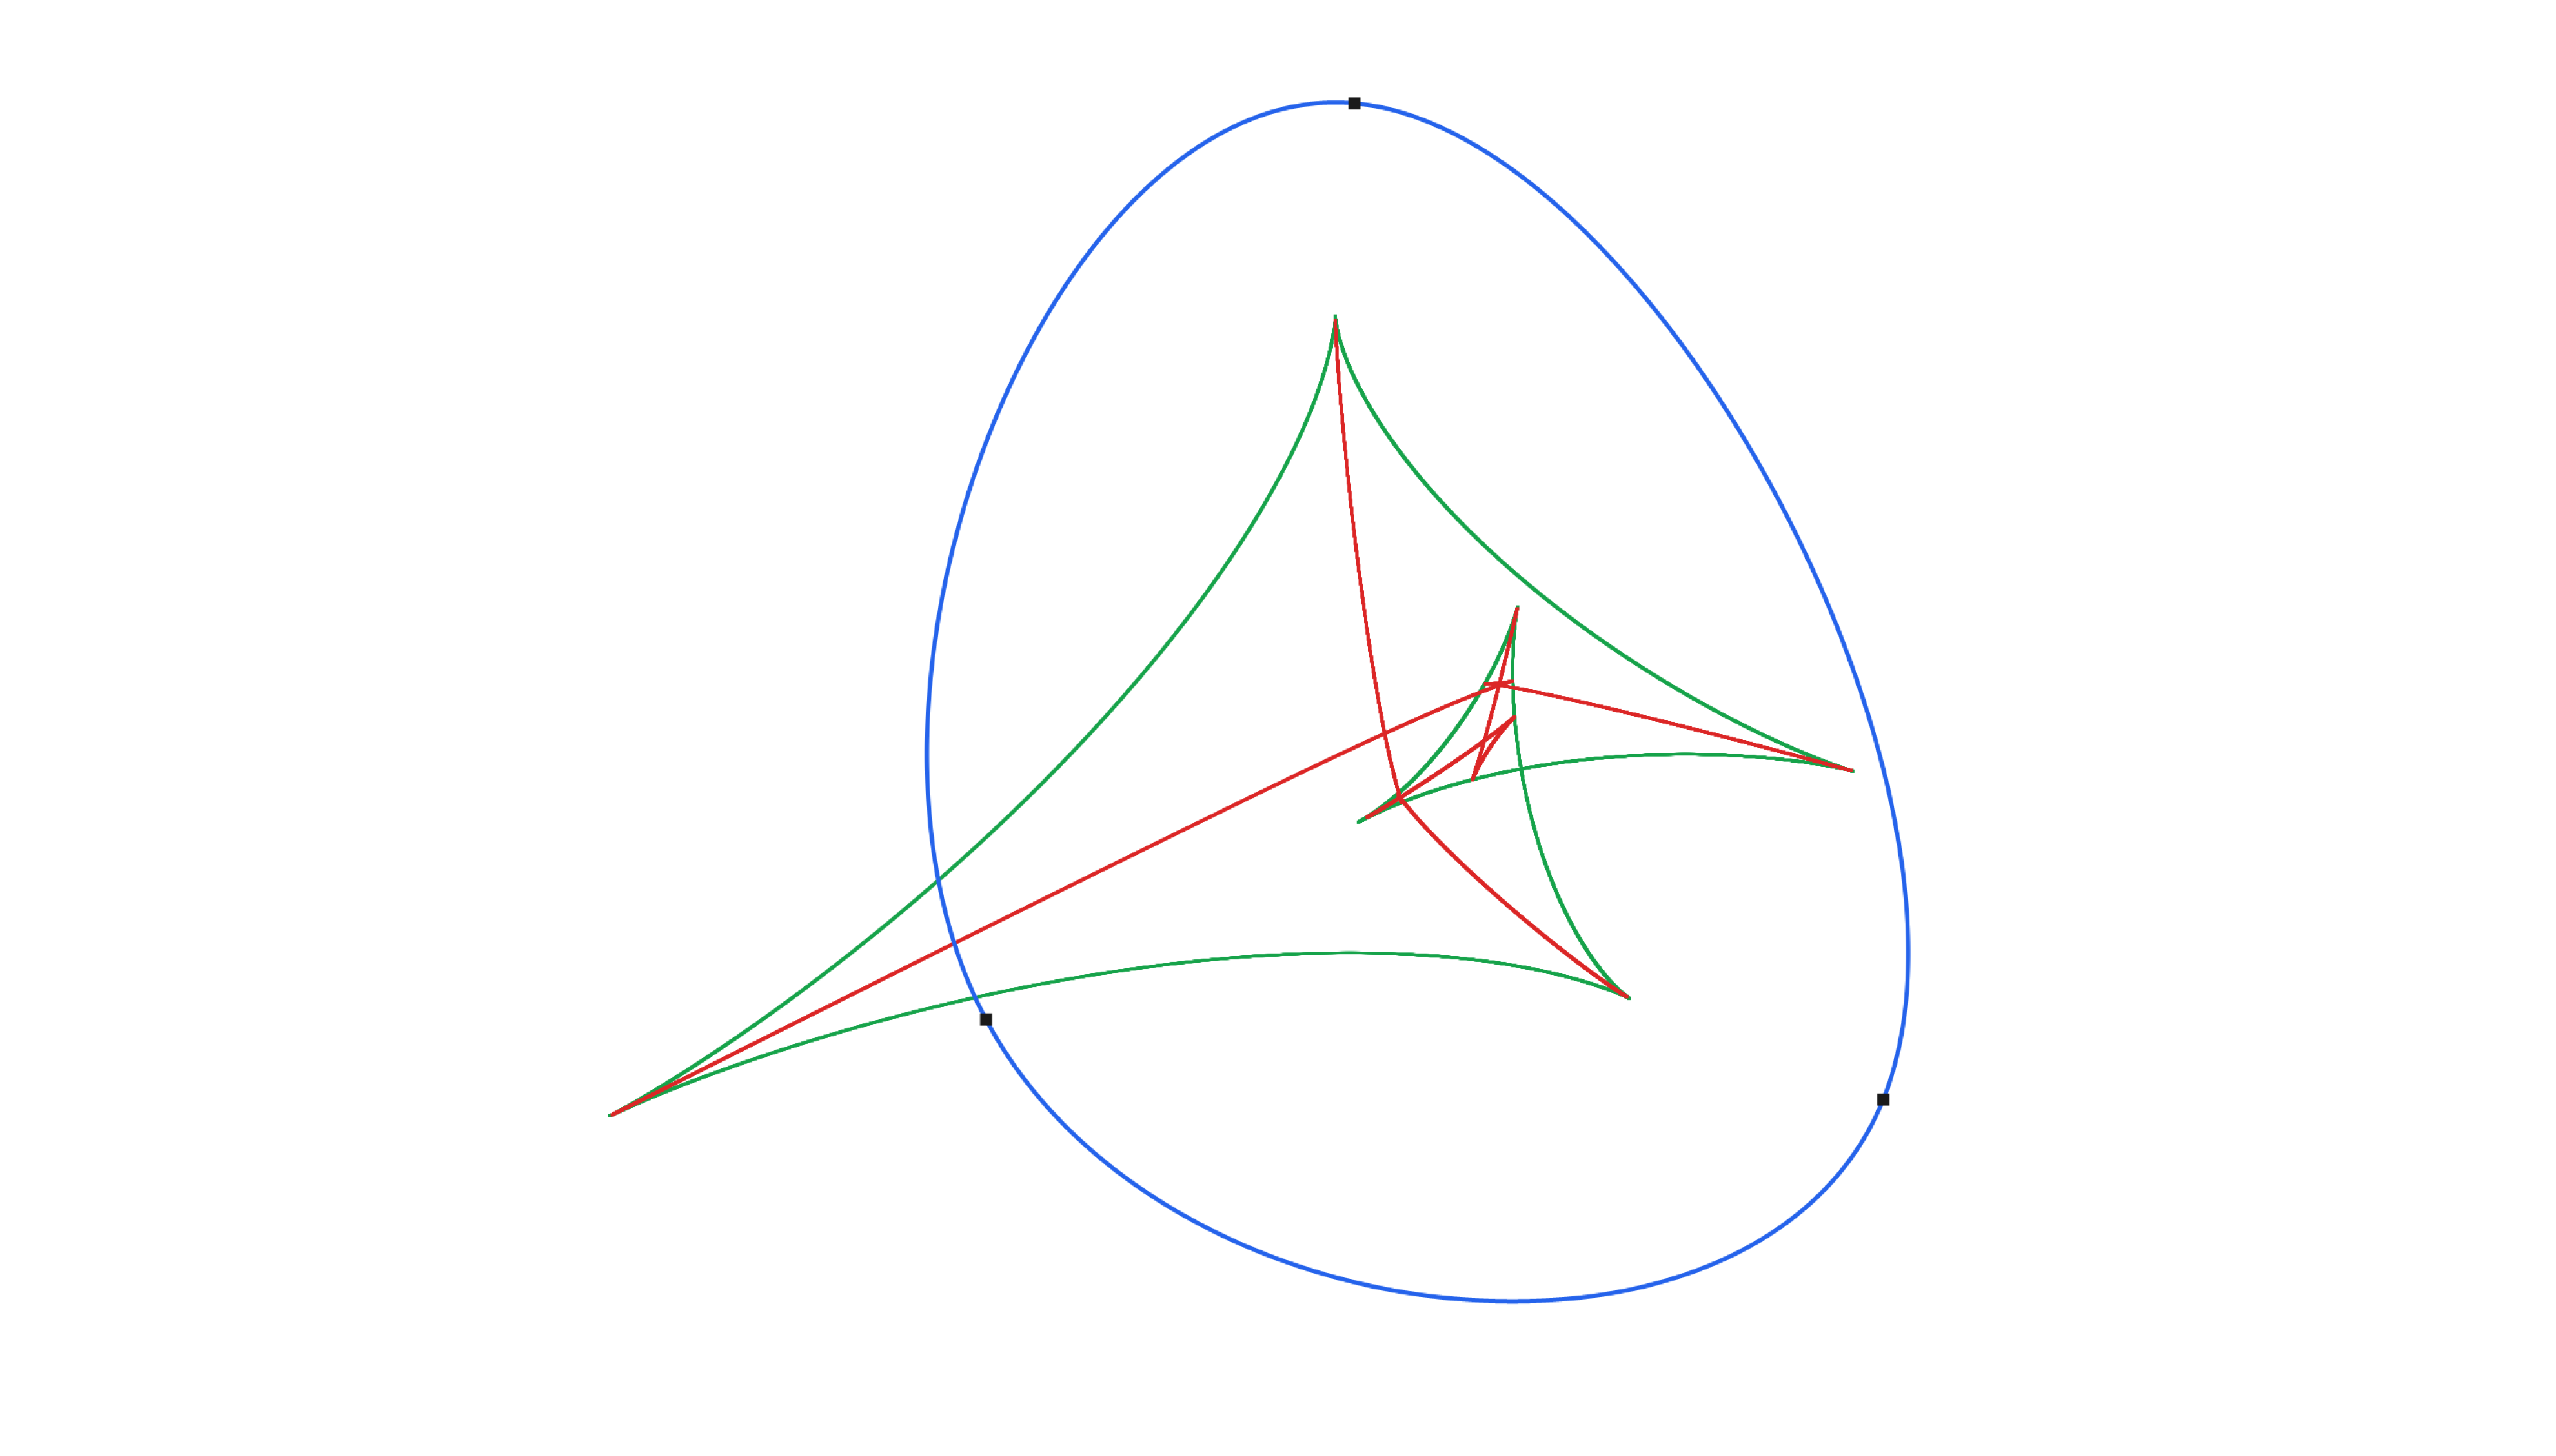
\includegraphics[width=0.8\textwidth]{focal_symmetry1.pdf}
    \caption{Visualizing the focal set (evolute) and symmetry set of a spline-defined curve $\mathcal{M}$. The green locus represents the evolute. The red locus represents the symmetry set.}
    \label{fig:focal_set_visualizer}
\end{figure}




\subsection{Vineyards}

A central component of our visualization is the concept of a \textit{vineyard}, which captures the continuous evolution of persistence diagrams as the filtration function changes. Introduced in  \cite{CohenSteiner2006}, vineyards provide a stable method for tracking topological features across a parameterized family of functions.
Let $\mathcal{M} \subset \mathbb{R}^2$ be a smooth manifold (curve) and let $\gamma:S^1\to\mathbb{R}^2$ be a closed curve. For each $t \in S^1$, define the radial distance function $f_t: \mathcal{M} \to \mathbb{R}$ by
\[
f_t(x) = d_{\mathbb{E}}^2(x,\gamma(t))|_\M.
\]

\begin{definition}[Vineyard]
The \textbf{vineyard} of the radial persistence transform, denoted $\mathcal{V}(\mathcal{M}, \gamma)$, is the subset of $S^1 \times \overline{\mathbb{R}}^2$ given by:
\[
\mathcal{V}(\mathcal{M}, \gamma) = \bigcup_{t \in S^1} \{t\} \times \mathrm{Dgm}(f_t)
\]
where $\mathrm{Dgm}(f_t)$ is the persistence diagram of the sublevel set filtration of $f_t$.
\end{definition}

The set $\mathcal{V}(\mathcal{M}, \gamma)$ decomposes into curves called \textit{vines}, which track individual persistence points as $t$ varies. In our tool, as the center point $\gamma(t)$ traverses the closed curve, vines trace the evolution of birth and death times of homological features.

\subsection{Monodromy}
Following a vine in a vineyard for an entire period, that is, traversing $S^1$ once, does not necessarily lead to the point in the persistence diagram you set out with. If this is the case, one says that there is monodromy. If $k>1$ is the smallest number such that following a (or each) vine while traversing the loop $k$ times you end up at the starting point in the persistence diagram, you say the monodromy is of order $k$.   




\section{Algorithm}

\subsection{Calculation of the Symmetry Set}

The Symmetry Set (SS) is the locus of centers of circles bitangent to a curve at two or more points. We are following the algorithm described in \cite{Bruce1985symmetry} for the computation of the symmetry set. Consider sampled points $\mathcal{P}=\{p_1,p_2,\dots, p_k\}$ from $\M$ and corresponding tangents $\{t_1,t_2,\dots,t_k\}$ and normals $\{n_1, n_2,\dots, n_k\}$ at these points. Algorithm \ref{alg:symmetry_set} describes our implementation.

\subparagraph{Bitangency Condition} 
We identify potential bitangencies by detecting zero-crossings of the functions:
\begin{equation*}
    f_{\pm}(i, j) = (p_i - p_j) \cdot (t_i \pm t_j)
\end{equation*}
A sign change in $f_{\pm}$ between adjacent samples $p_j, p_{j+1}$ indicates a local bitangent condition.

\subparagraph{Intersection Calculation}
When a zero-crossing is detected, the center $C$ is found by intersecting the normal lines $L_i = p_i + \lambda n_i$ and $L_j = p_j + \mu n_j$. We solve for $\lambda$ by projecting the  $(p_i-p_j)$ onto the combined normal vector:
\begin{equation*}
    \lambda = \frac{-(p_i - p_j) \cdot (n_i \pm n_j)}{\|n_i \pm n_j\|^2}
\end{equation*}
The candidate center is $C = p_i + \lambda n_i$. We retain $C$ only if it satisfies the equidistance constraint $|\|C-p_i\| - \|C-p_j\|| < \epsilon_{rad}$, which ensures numerical stability against discretization artifacts.

\begin{algorithm}[t]
\caption{Discrete Symmetry Set Computation}
\label{alg:symmetry_set}
\DontPrintSemicolon
\KwIn{Sampled curve points $\mathcal{P} = \{p_1, \dots, p_k\}$ with tangents $\{t_1, \dots, t_k\}$ and normals $\{n_1, \dots, n_k\}$. Thresholds $\epsilon_{chord}, \epsilon_{rad}$.}
\KwOut{List of Symmetry Set centers $\mathcal{S}$}

$\mathcal{S} \gets \emptyset$\;
\For{$i \gets 1$ \textbf{to} $k$}{
    $v_{prev}^{\pm} \gets \text{NaN}$\;
    \For{$j \gets i+1$ \textbf{to} $k$}{
        $\Delta p \gets p_i - p_j$\;
        \lIf{$\|\Delta p\|^2 < \epsilon_{chord}$}{\textbf{continue}}

        \tcp{Check tangent condition: $\Delta p \cdot (t_i \pm t_j) = 0$}
        \If{$|{t_i \cdot t_j}| < 1 - \epsilon$}{ 
            $v_{curr}^{\pm} \gets \Delta p \cdot (t_i \pm t_j)$\;
            \If{$v_{prev}^{\pm} \cdot v_{curr}^{\pm} < 0$}{
                \tcp{Sign change detected: Normals approx intersect}
                $C \gets \text{ComputeIntersection}(p_i, n_i, p_j, n_j)$\;
                $r_i \gets \|C - p_i\|, \quad r_j \gets \|C - p_j\|$\;
                \If{$|r_i - r_j| < r_i \cdot \epsilon_{rad}$}{
                    $\mathcal{S} \gets \mathcal{S} \cup \{C\}$\;
                }
            }
            $v_{prev}^{\pm} \gets v_{curr}^{\pm}$\;
        }
    }
}
\Return{$\mathcal{S}$}
\end{algorithm}

\subsection{Vineyard Computation}

The vineyard $\mathcal{V}$ is constructed by stack-wise concatenation of persistence diagrams generated from a parameterized family of distance functions. Methods have been proposed by e.g. \cite{tamalrevisit} to compute vineyards effectively, but an elementary approach suffices here.\footnote{Because working with curves in 2D means the efficient union find algorithm suffices to compute the persistence diagram, which is sufficiently fast, not to require more sophisticated tools to further speed-up.} %we go for a more primitive approach. 
In our tool, we parameterize the filtration by moving the source point $\gamma(t)$ along a circular path of user-defined radius and center, or an arbitrary user-drawn loop via splines \cite{deBoor1978}.

\subparagraph{Persistence}
For a fixed $t$, we compute persistence using a Union-Find based algorithm on the lower star filtration of the squared distance function $f_\theta(p) = d_{\mathbb{E}}^2(p,\gamma(t))|_\M$. As we iterate through points $p \in \mathcal{P}$ in increasing order of distance, components are merged. The ``Elder Rule'' is applied to pair the birth time (distance) of a merging component with the current distance as its death time.

\subparagraph{Vine Tracking}
The tool captures the evolution of these birth-death pairs across $m$ discrete samples of $t \in S^1$. The resulting collection of points in $(t, \text{birth}, \text{death})$ space forms the vines. By visualizing these vines, the user can observe the \textit{braiding} of topological features, in accordance with \cite{chambers2025braidingvineyards}.
%which characterizes the monodromy of the radial persistence transform for the given shape.

% \begin{algorithm}[H]
% \caption{Vineyard Computation via Circular Filtration}
% \label{alg:vineyard}
% \DontPrintSemicolon
% \SetAlgoNoEnd 
% \KwIn{Curve points $\mathcal{P}$, center $C$, radius $R$, number of samples $m$.}
% \KwOut{Vineyard $\mathcal{V} = \{ \text{Dgm}(\theta_i) \}_{i=1}^m$}

% $\mathcal{V} \gets \emptyset$\;
% \For{$i \gets 0$ \textbf{to} $m-1$}{
%     $\theta_i \gets \frac{2\pi i}{m}$\;
%     $c_i \gets (C.x + R \cos\theta_i, C.y + R \sin\theta_i)$ \tcp*{Shifted filtration center}
    
%     \tcp{Compute 0D Persistence via Lower Star Filtration}
%     $D \gets \text{array of squared distances } \|p - c_i\|^2 \text{ for } p \in \mathcal{P}$\;
%     $V_{sorted} \gets \text{indices of } \mathcal{P} \text{ sorted by } D$\;
%     $UF \gets \text{Union-Find data structure}$\;
%     $Dgm \gets \emptyset$\;
    
%     \For{$v \in V_{sorted}$}{
%         \For{$u \in \text{Neighbors}(v)$}{
%             \If{$u$ is already processed}{
%                 \If{$UF.find(u) \neq UF.find(v)$}{
%                     $birth \gets \text{depth of merged component}$\;
%                     $Dgm \gets Dgm \cup \{(birth, D[v])\}$\;
%                     $UF.union(u, v)$\;
%                 }
%             }
%         }
%     }
%     $\mathcal{V} \gets \mathcal{V} \cup \{(\theta_i, Dgm)\}$\;
% }
% \Return{$\mathcal{V}$}
% \end{algorithm}

% \section{Examples}

% \setlength{\fboxrule}{0.4pt}   % thin border
% \setlength{\fboxsep}{0pt}     % no padding between image and border

\section{Examples and Demonstration}

To demonstrate the utility of our tool, we present a series of visualizations highlighting the interplay between the geometry of the input curve $\mathcal{M}$ and its vineyard topology.

\subsection{Symmetry and Focal Sets of Deforming Ellipses}
We begin by validating our tool against known geometric behaviors. Figure \ref{fig:dented_ellipse} illustrates the evolution of the focal and symmetry sets for a family of ellipse-like shapes, inspired by the work of \cite{WrongVersionGiblin}. As the ellipse is deformed from a convex shape into a non-convex ``bean'' shape, we observe the characteristic bifurcations in the symmetry set (red) and the formation of cusps in the focal set (green). The tool accurately captures the emergence of ``swallowtail'' singularities in the focal set, which correspond to the creation of inflection points on the curve, as shown in \cite{giblin2003symmetry}.

\begin{figure}[htbp]
    \centering
    \fcolorbox{gray!60}{white}{%
    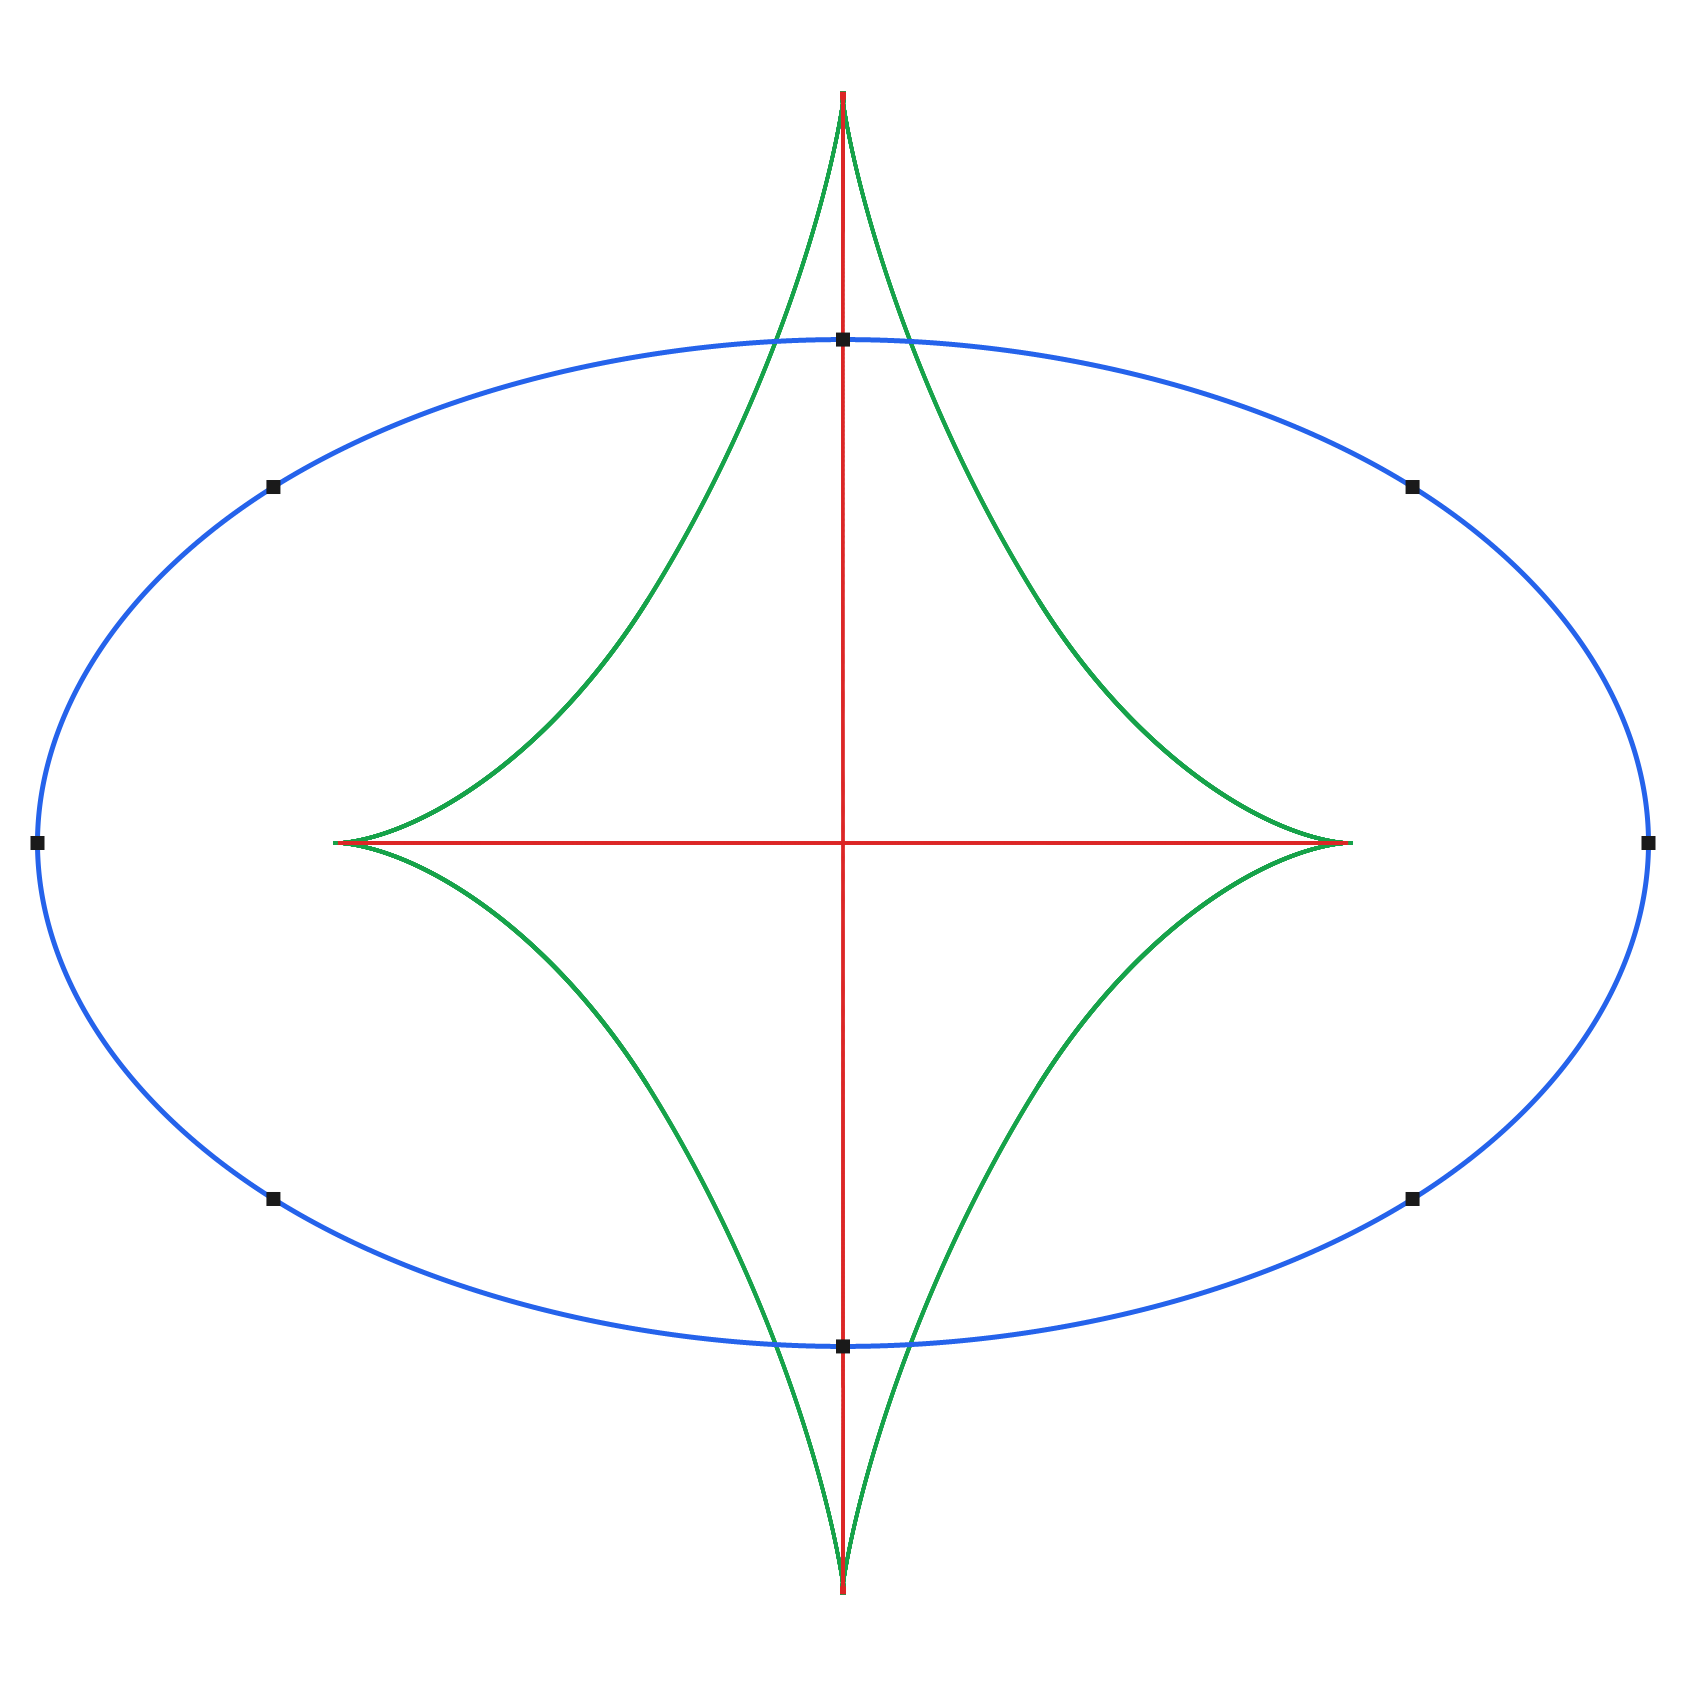
\includegraphics[width=0.47\linewidth]{figures/ellipse_deform1.png}}
    \hfill
    \fcolorbox{gray!60}{white}{%
    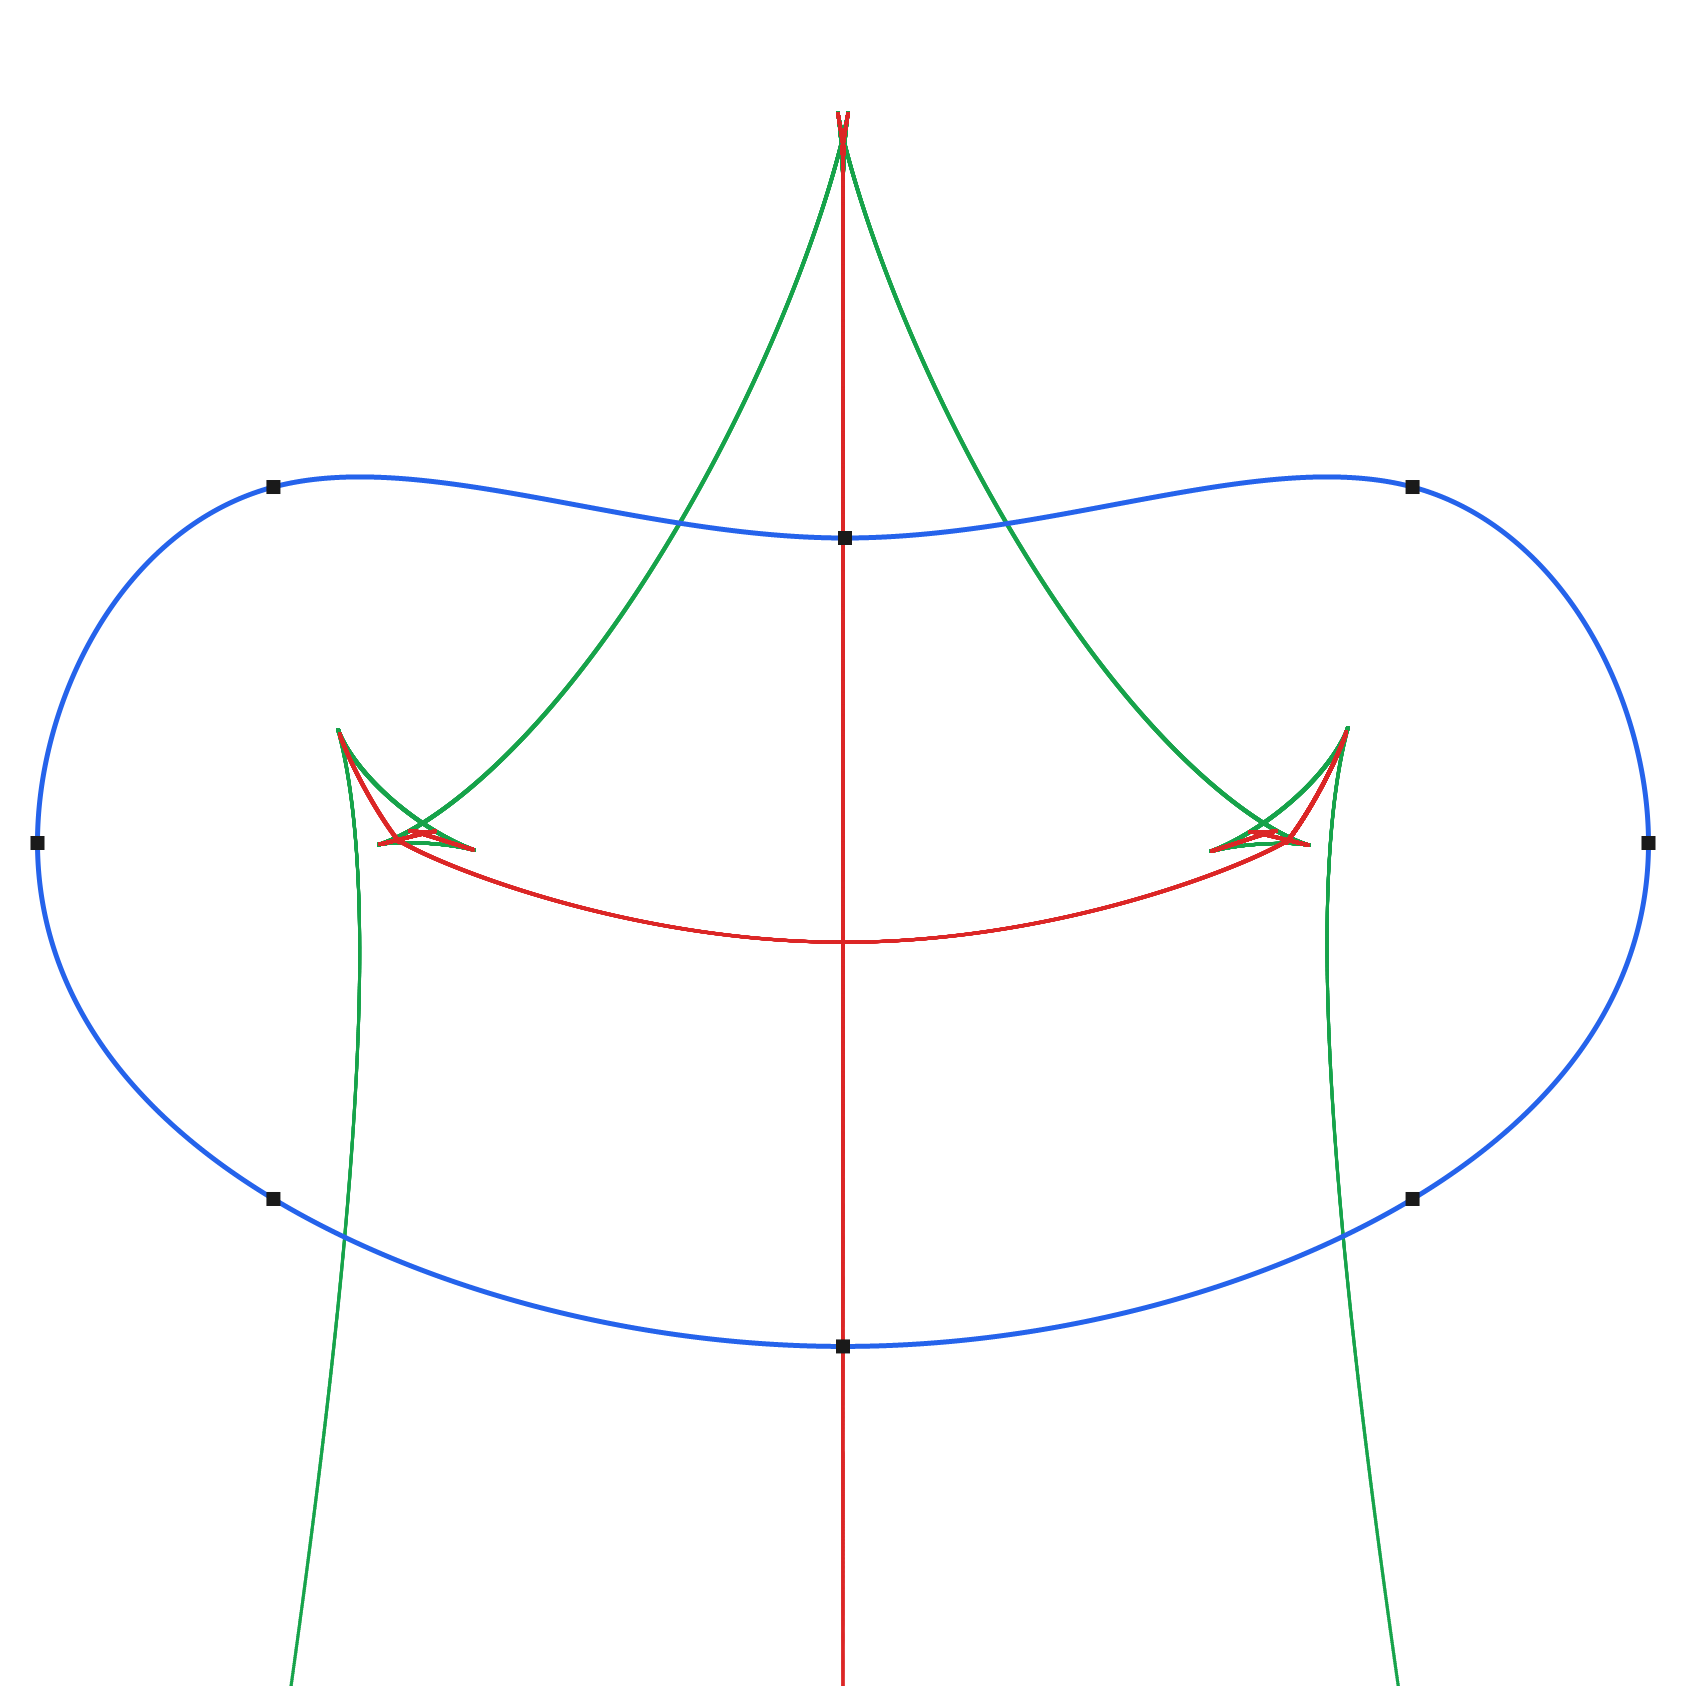
\includegraphics[width=0.47\linewidth]{figures/ellipse_deform2.png}}

    \fcolorbox{gray!60}{white}{%
    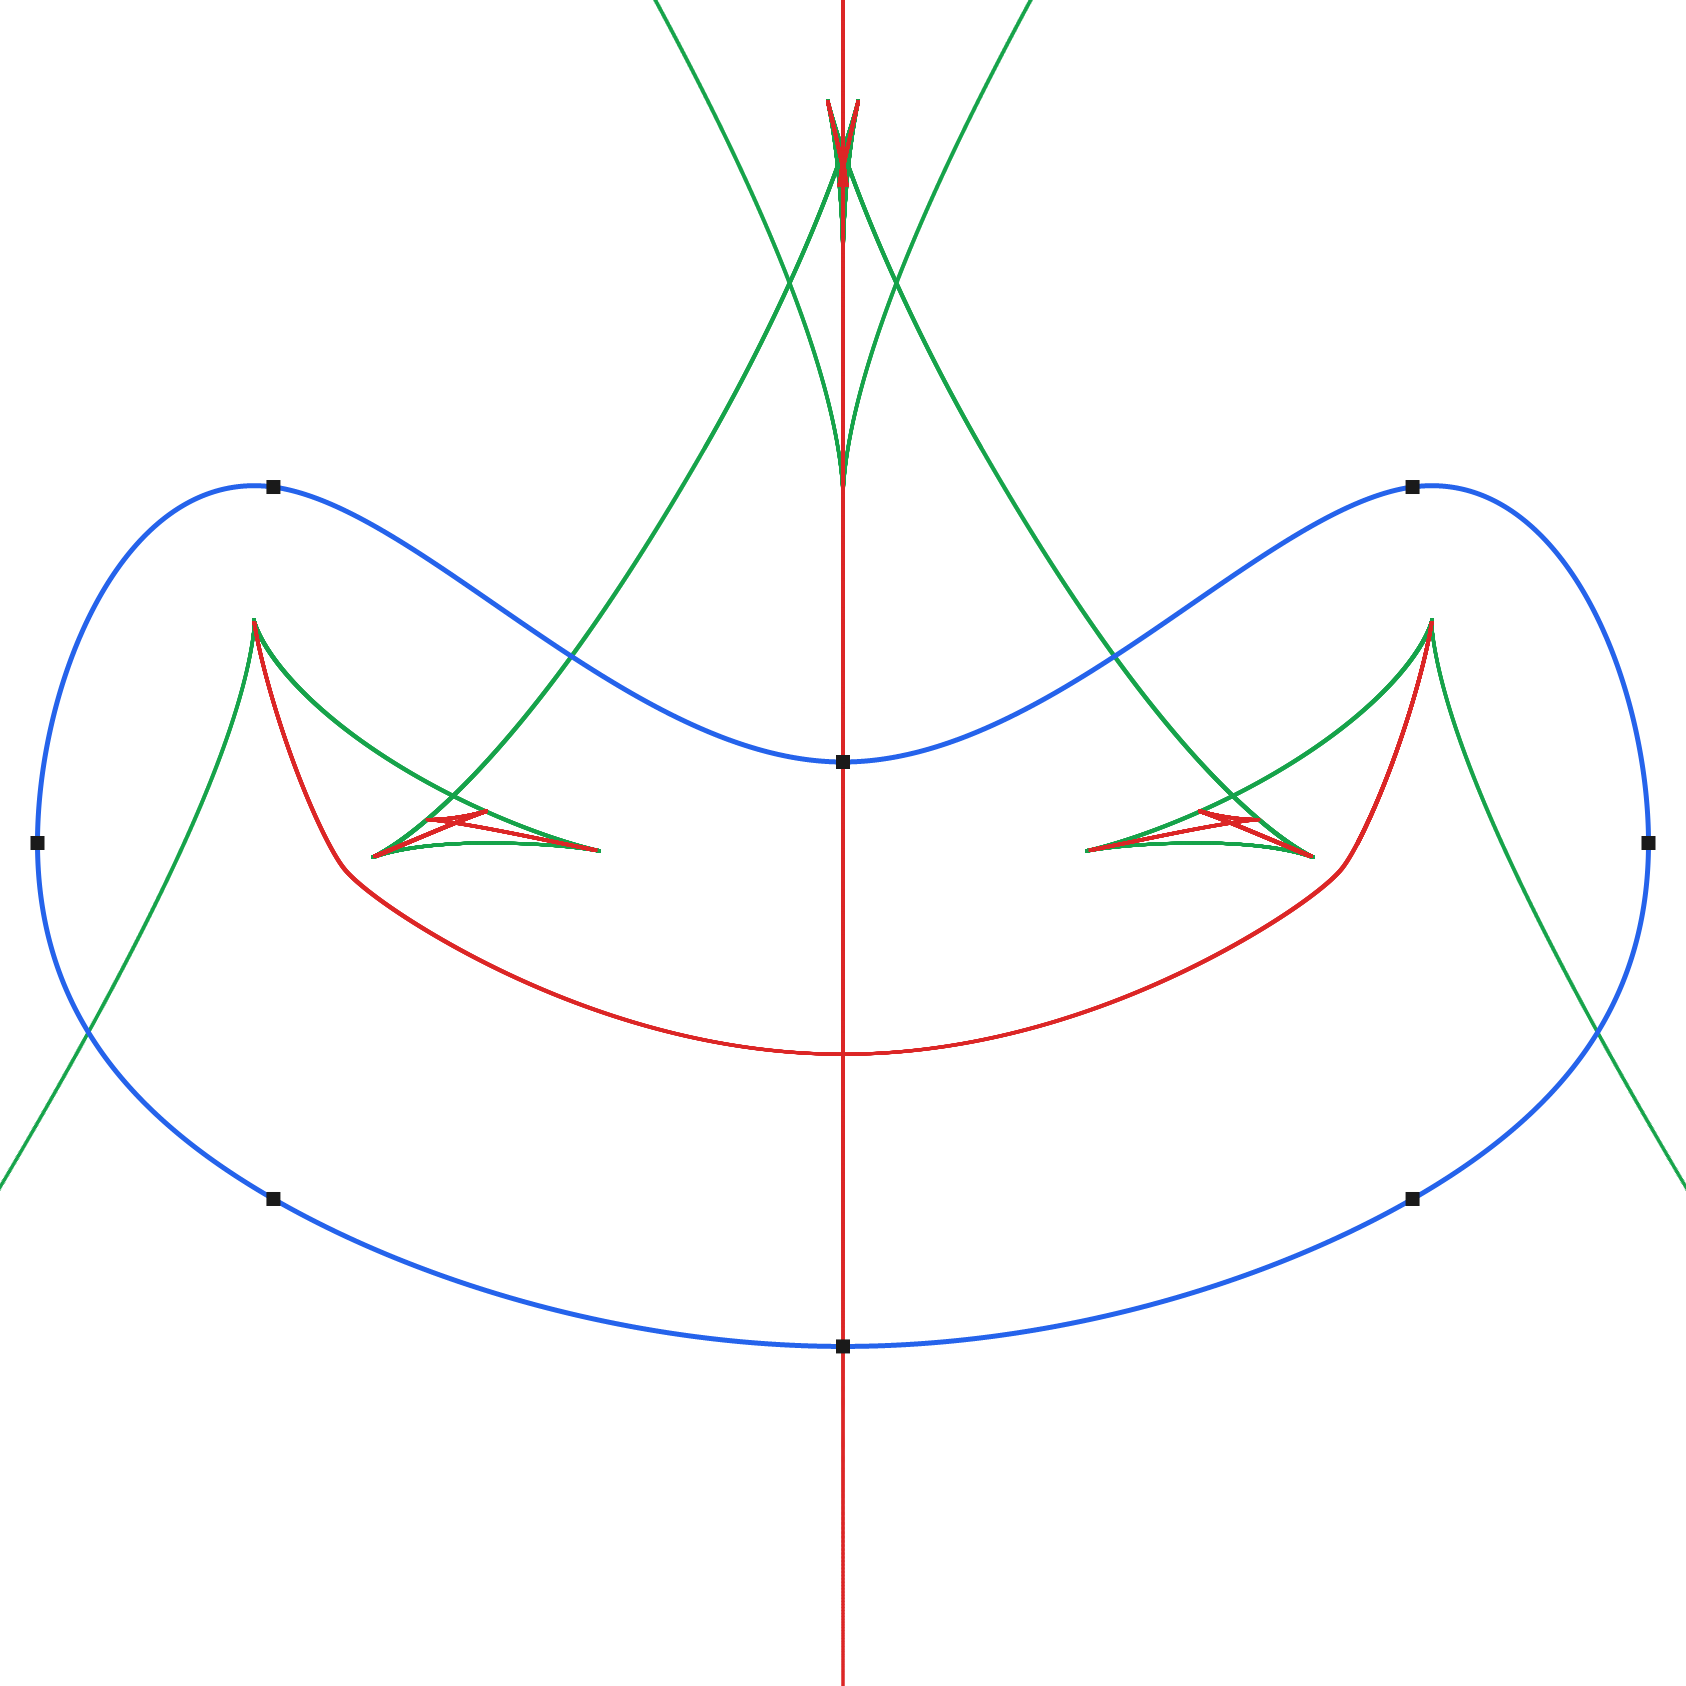
\includegraphics[width=0.47\linewidth]{figures/ellipse_deform3.png}}
    \hfill
    \fcolorbox{gray!60}{white}{%
    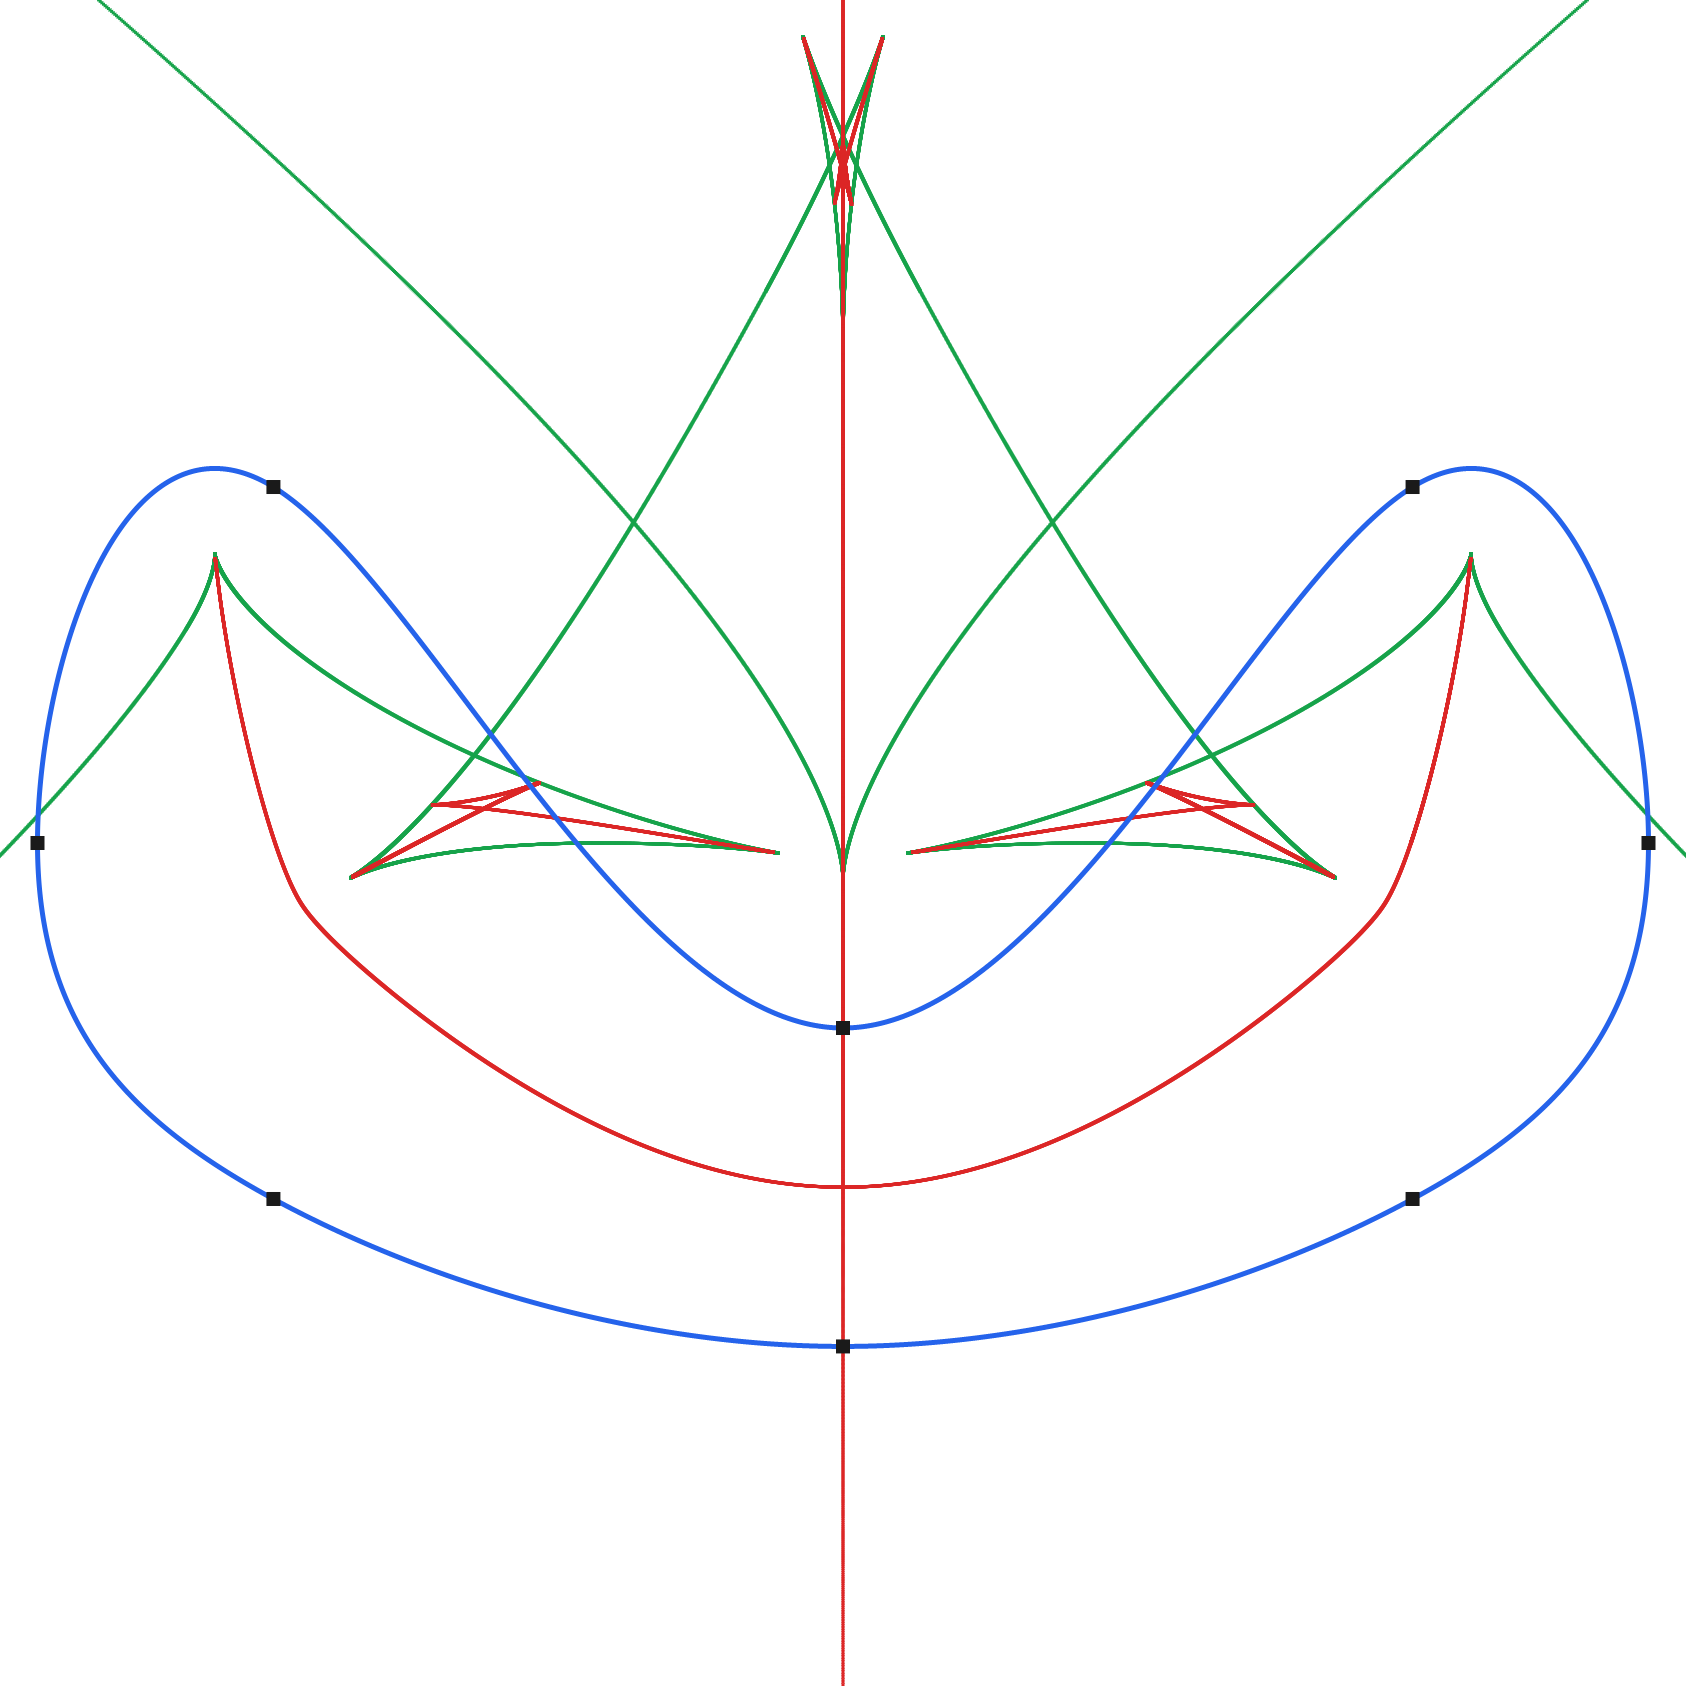
\includegraphics[width=0.47\linewidth]{figures/ellipse_deform4.png}}
    \caption{Focal (green) and symmetry (red) sets of ellipses undergoing deformation (inspired from \cite{WrongVersionGiblin}). The sequence captures the transition from a pure ellipse to a non-convex shape, showing the creation of cusps and self-intersections in the singularity sets.}
    \label{fig:dented_ellipse}
\end{figure}

\subsection{Complexity in Arbitrary Splines}
The tool's robustness is further tested on complex, hand-picked spline curves (Figure \ref{fig:fun_pics}). Even for highly non-convex shapes with multiple lobes, the discrete algorithm successfully resolves intricate symmetry set branches and the global structure of the focal set. Furthermore, the tool is capable of handling inputs with multiple connected components. As seen in the bottom right of Figure \ref{fig:fun_pics}, the visualization captures not only the local symmetry within each individual curve but also the global bitangential interactions \textit{between} the two disjoint shapes.
% This visualization underscores the difficulty of inferring global symmetry from local features alone, as distant parts of the curve interact to form dense bitangency networks.

\begin{figure}
    \centering
    \fcolorbox{gray!60}{white}{%
        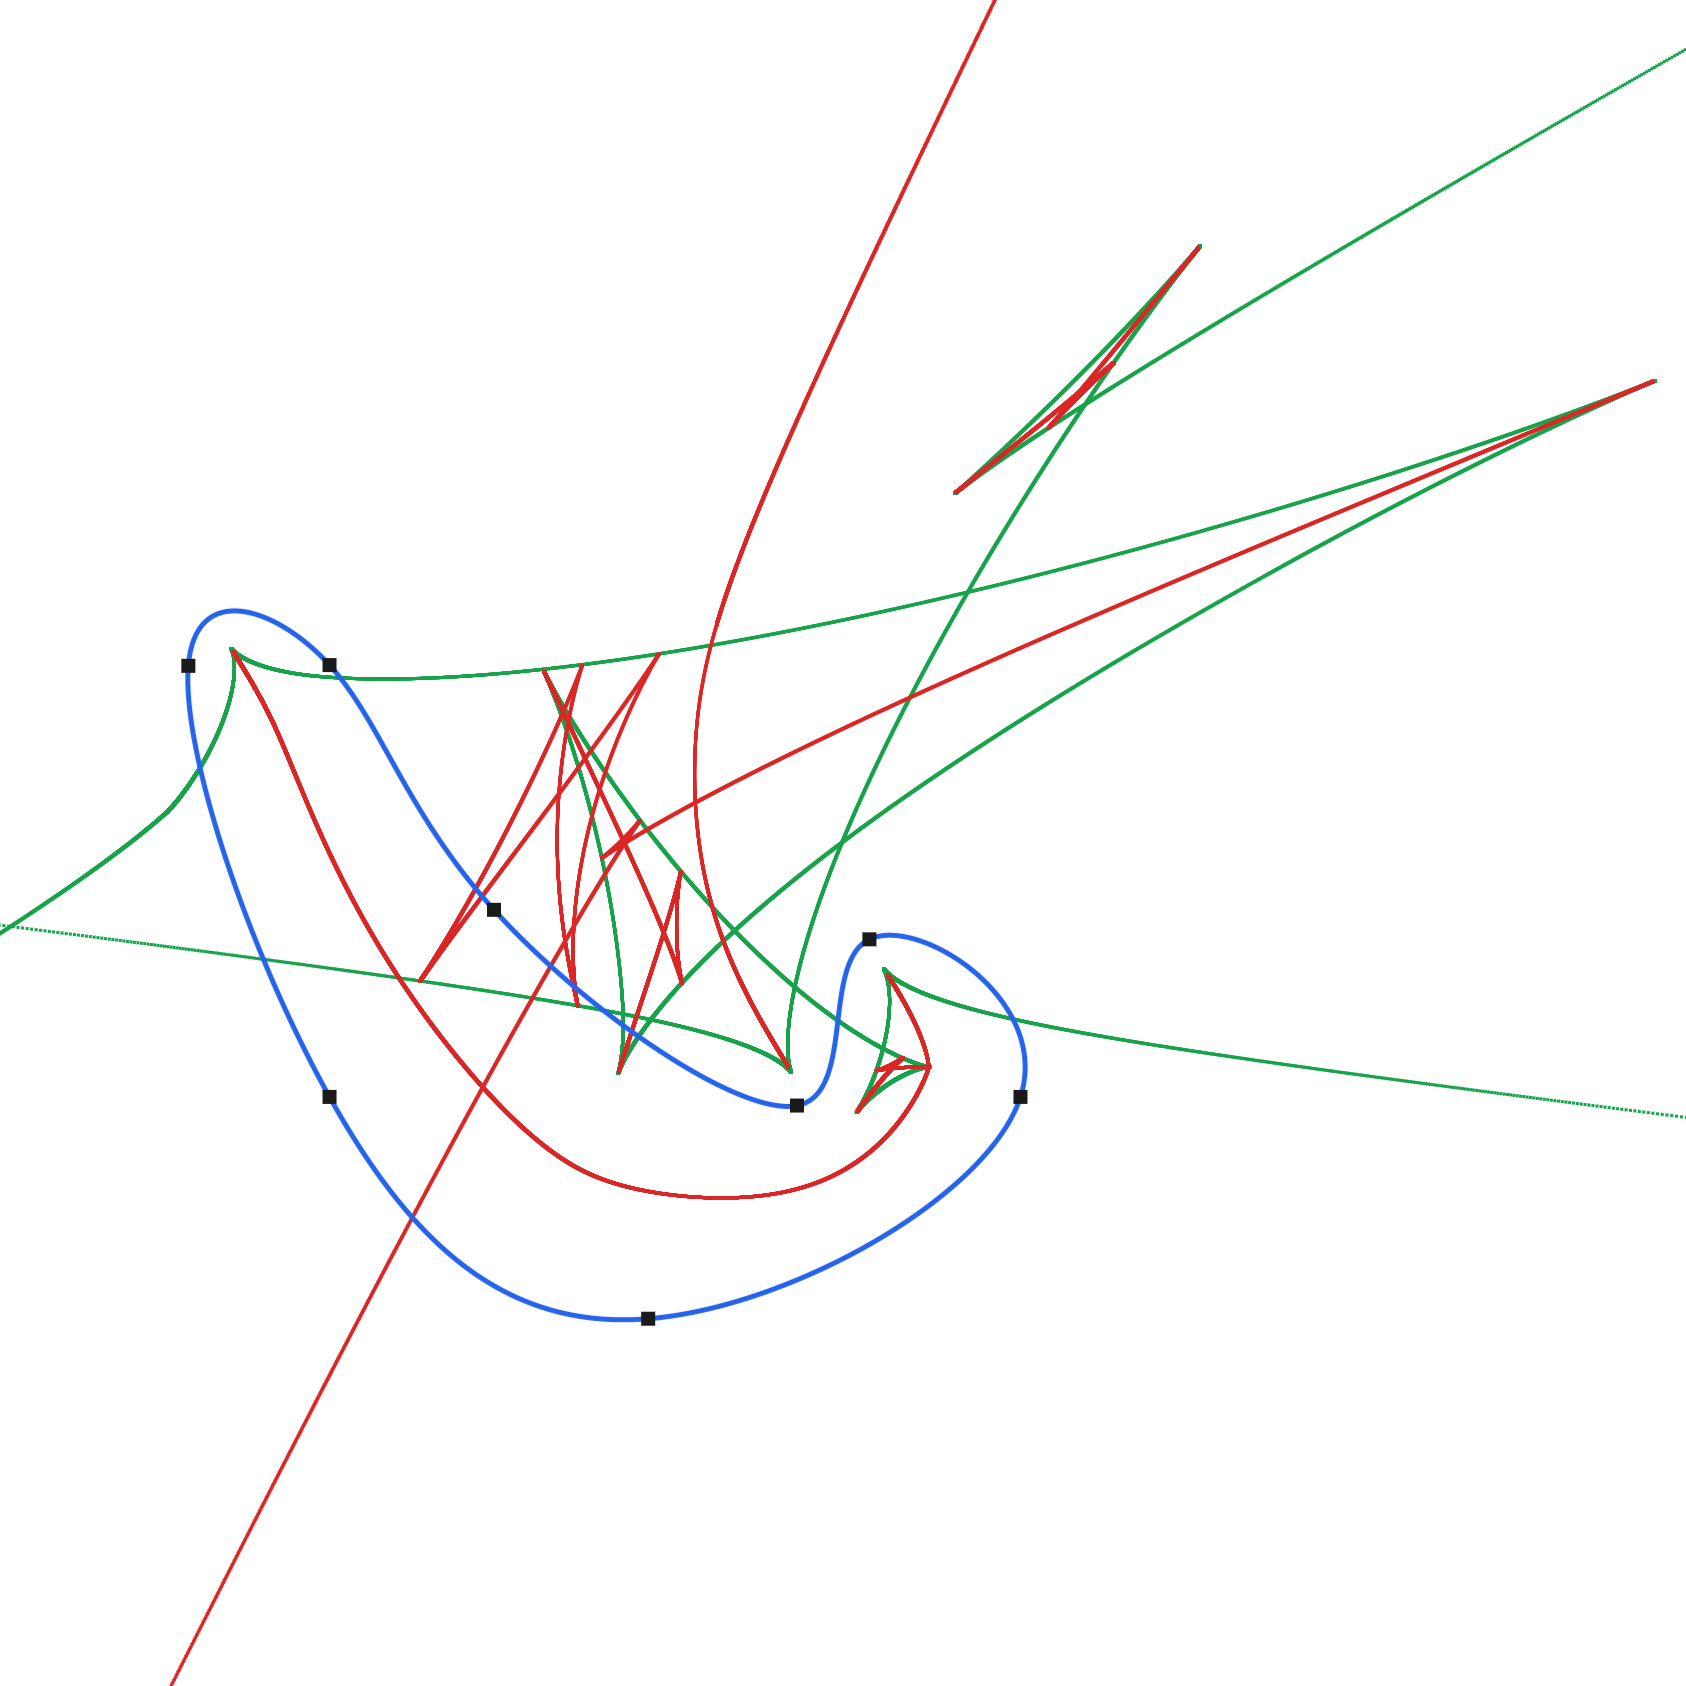
\includegraphics[width=0.47\linewidth]{figures/fun1.png}}
    \hfill
    \fcolorbox{gray!60}{white}{%
        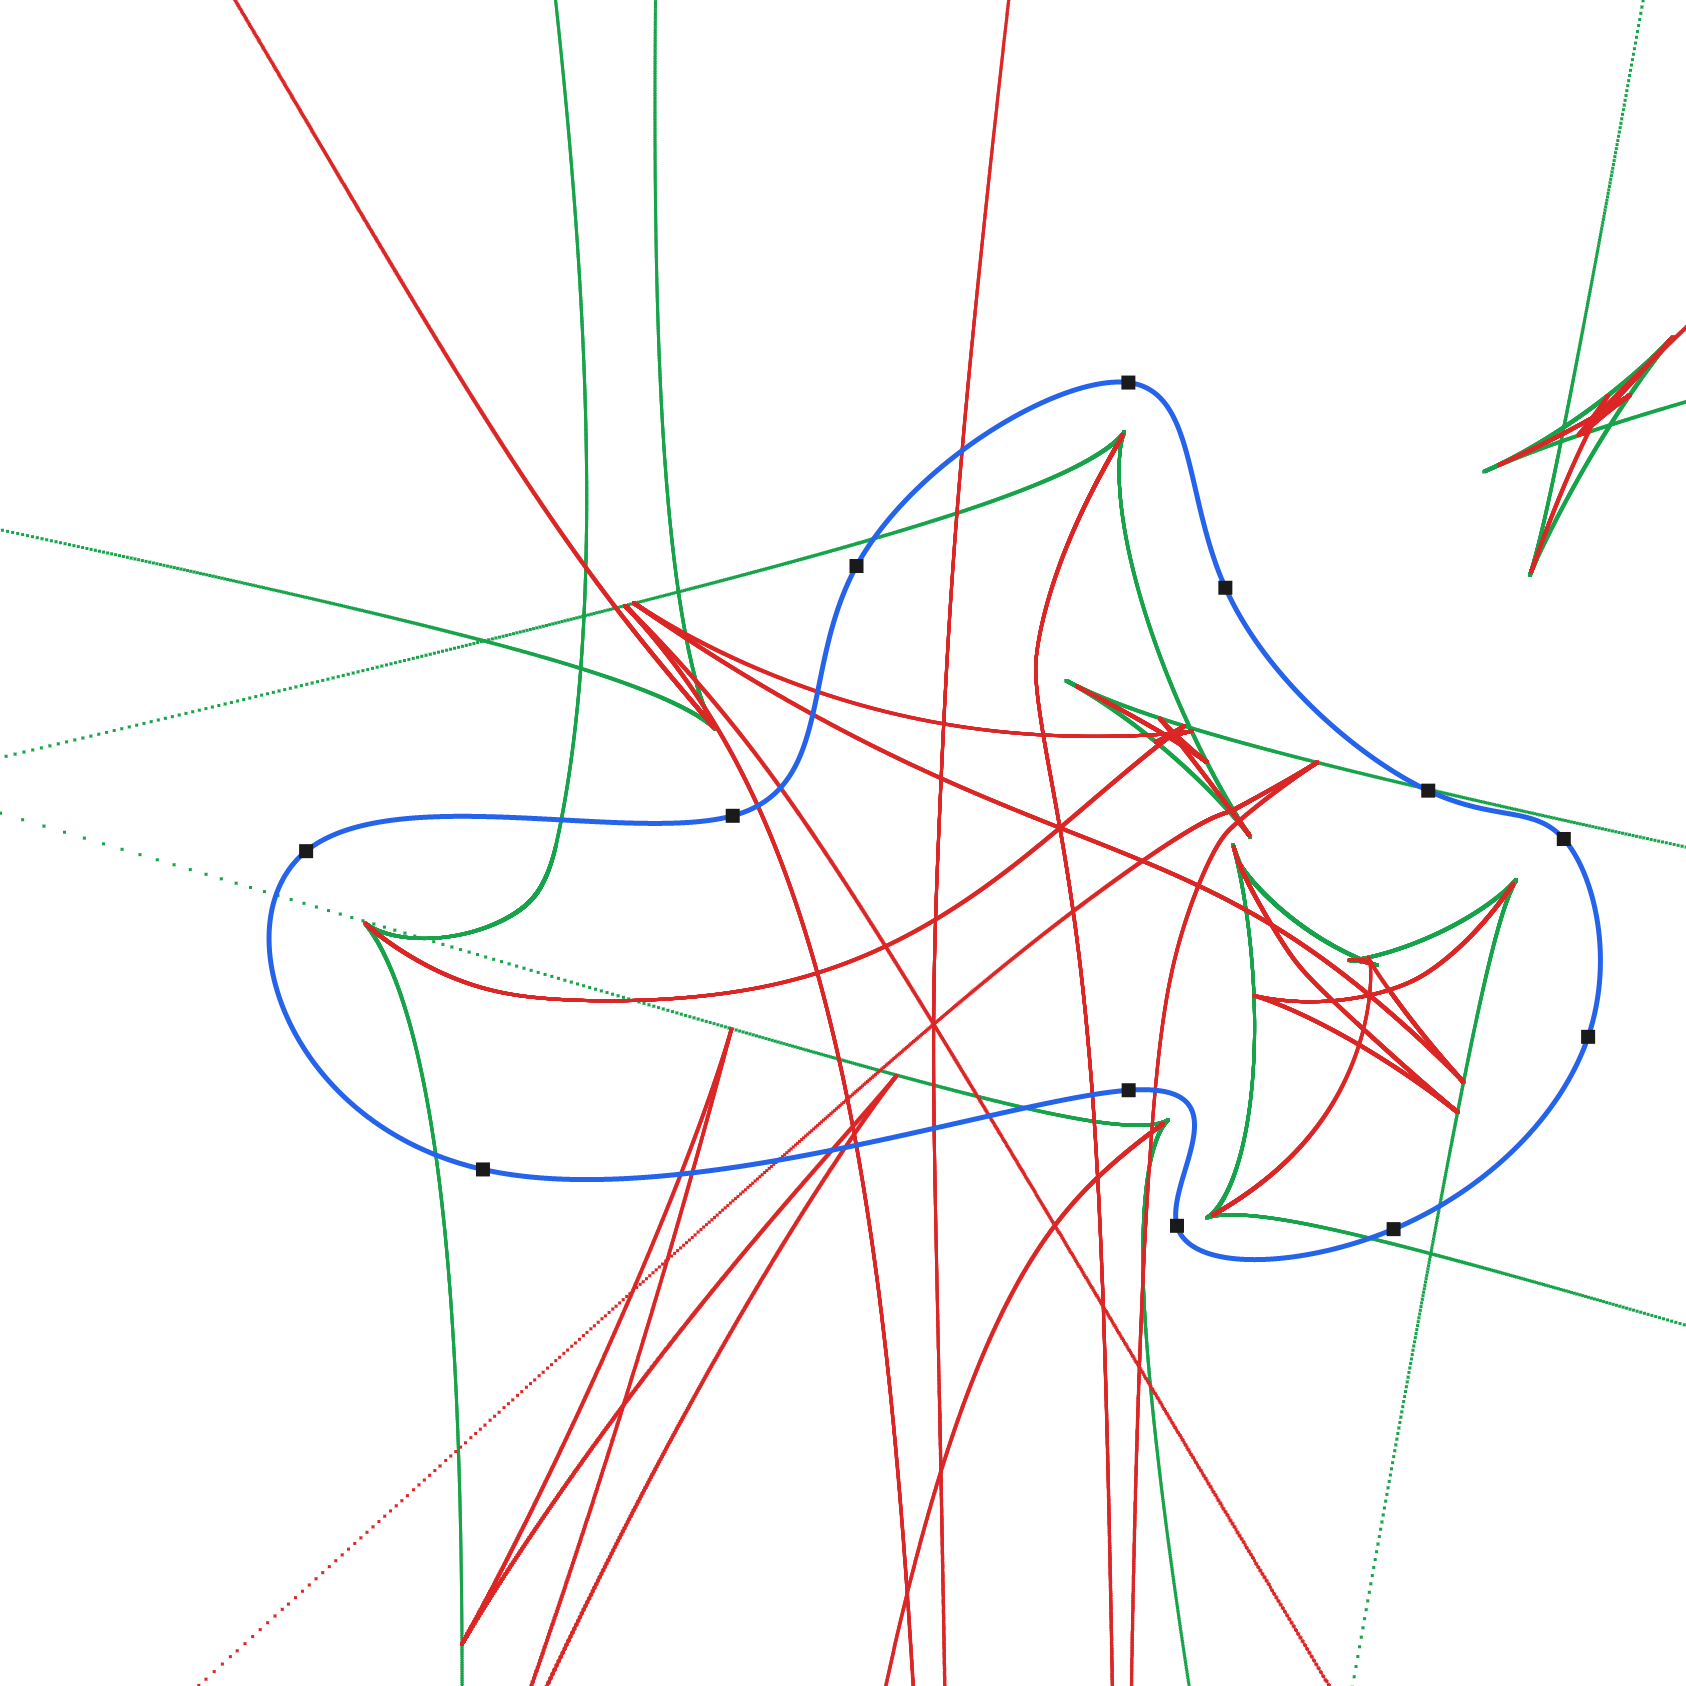
\includegraphics[width=0.47\linewidth]{figures/fun2.png}}
    \vspace{0.8em} % vertical separation between rows
    \fcolorbox{gray!60}{white}{%
        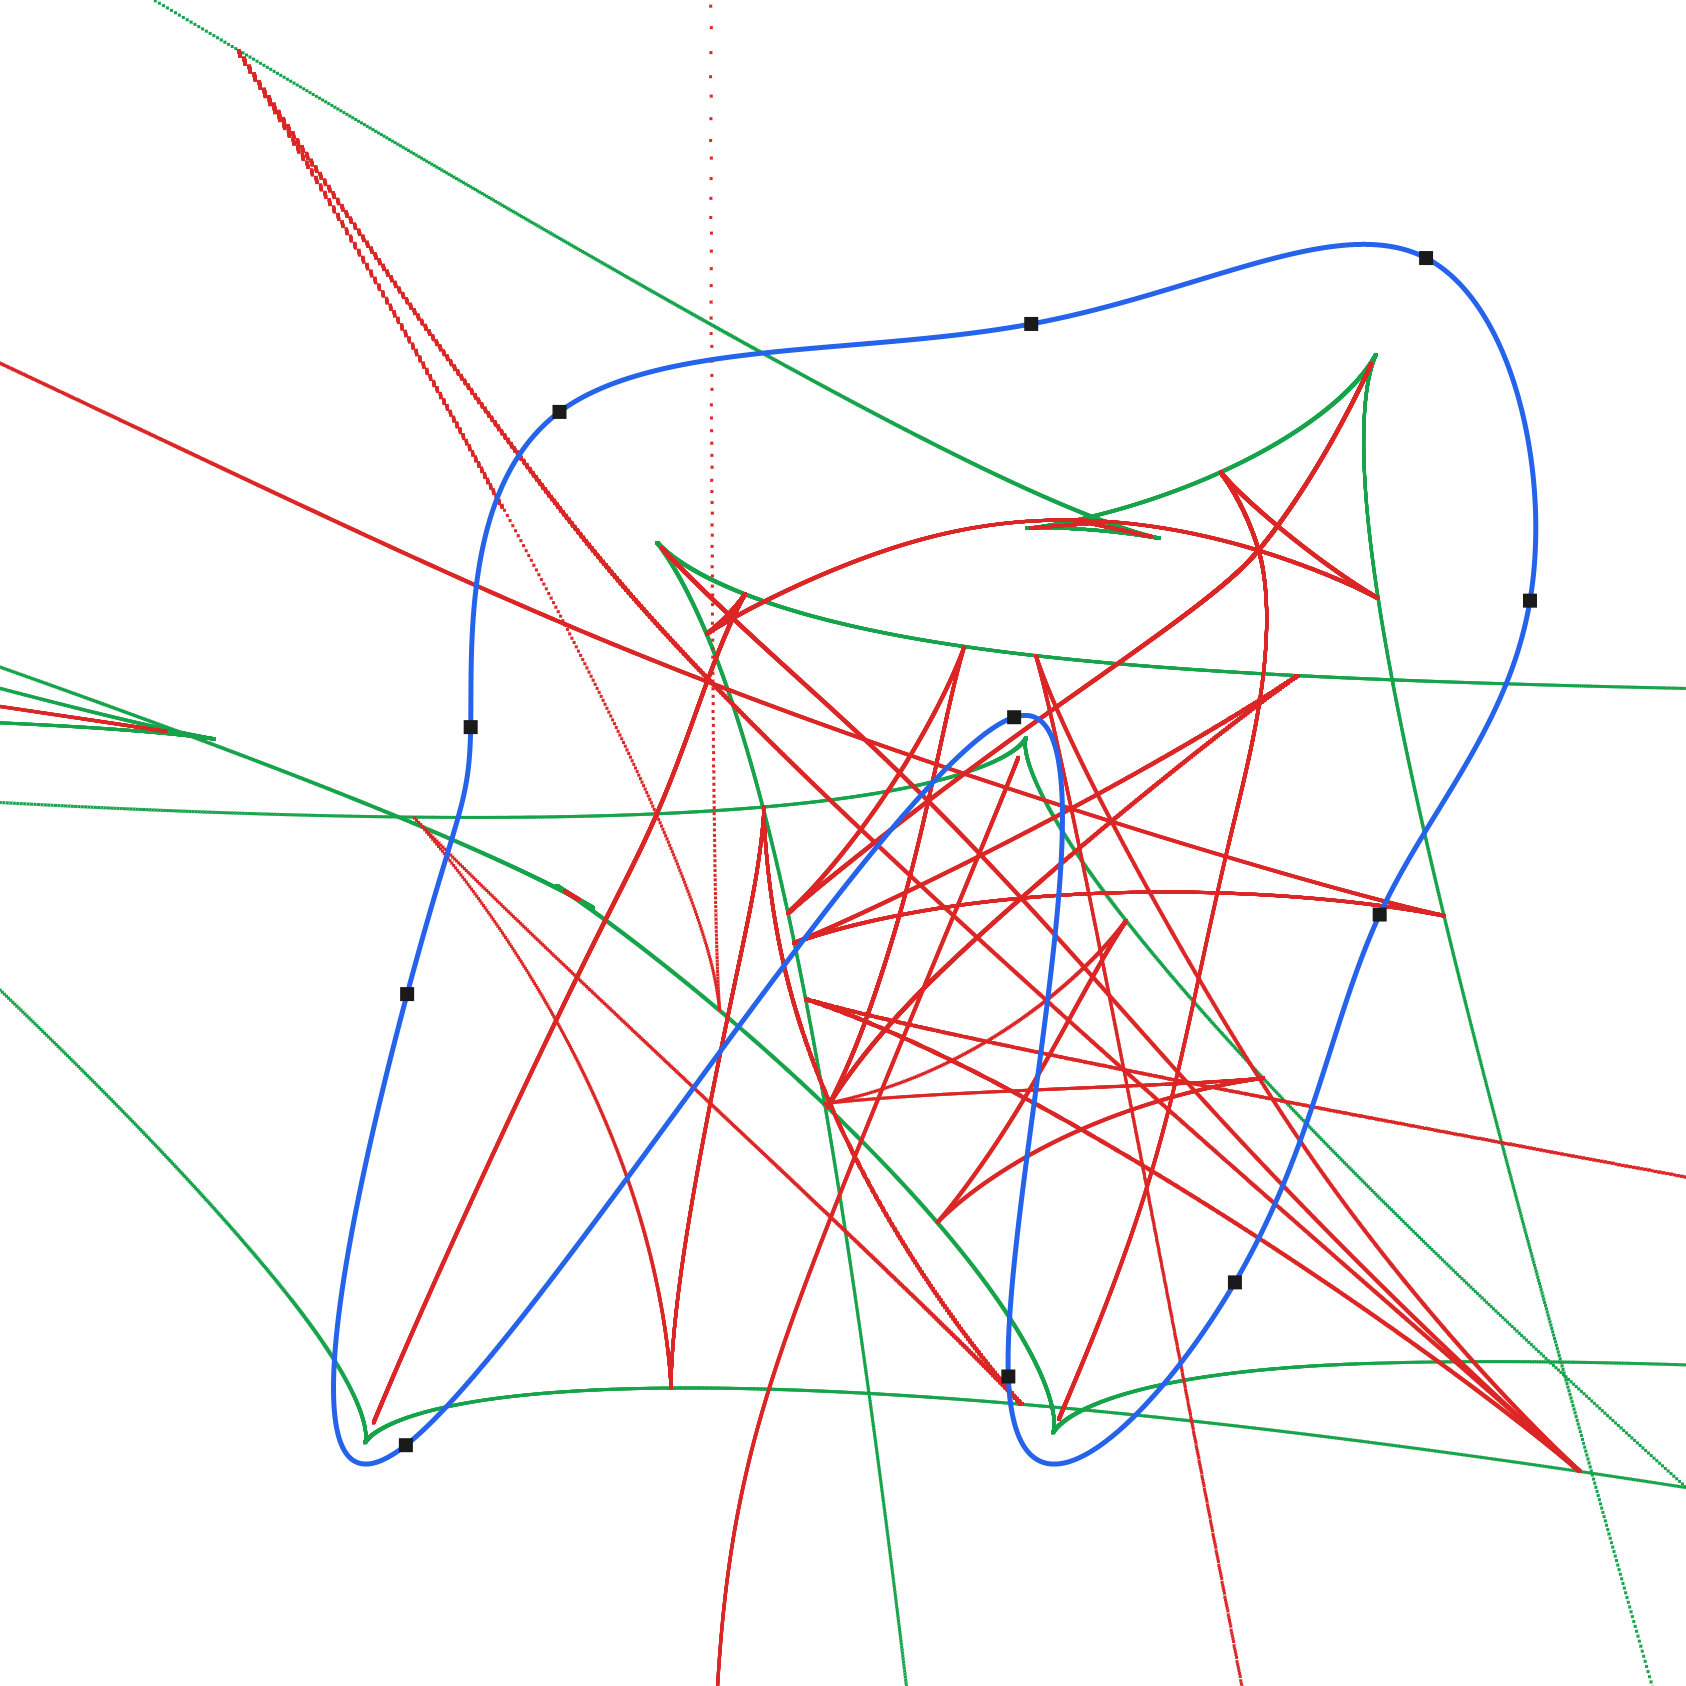
\includegraphics[width=0.47\linewidth]{figures/fun3.png}}
    \hfill
    \fcolorbox{gray!60}{white}{%
        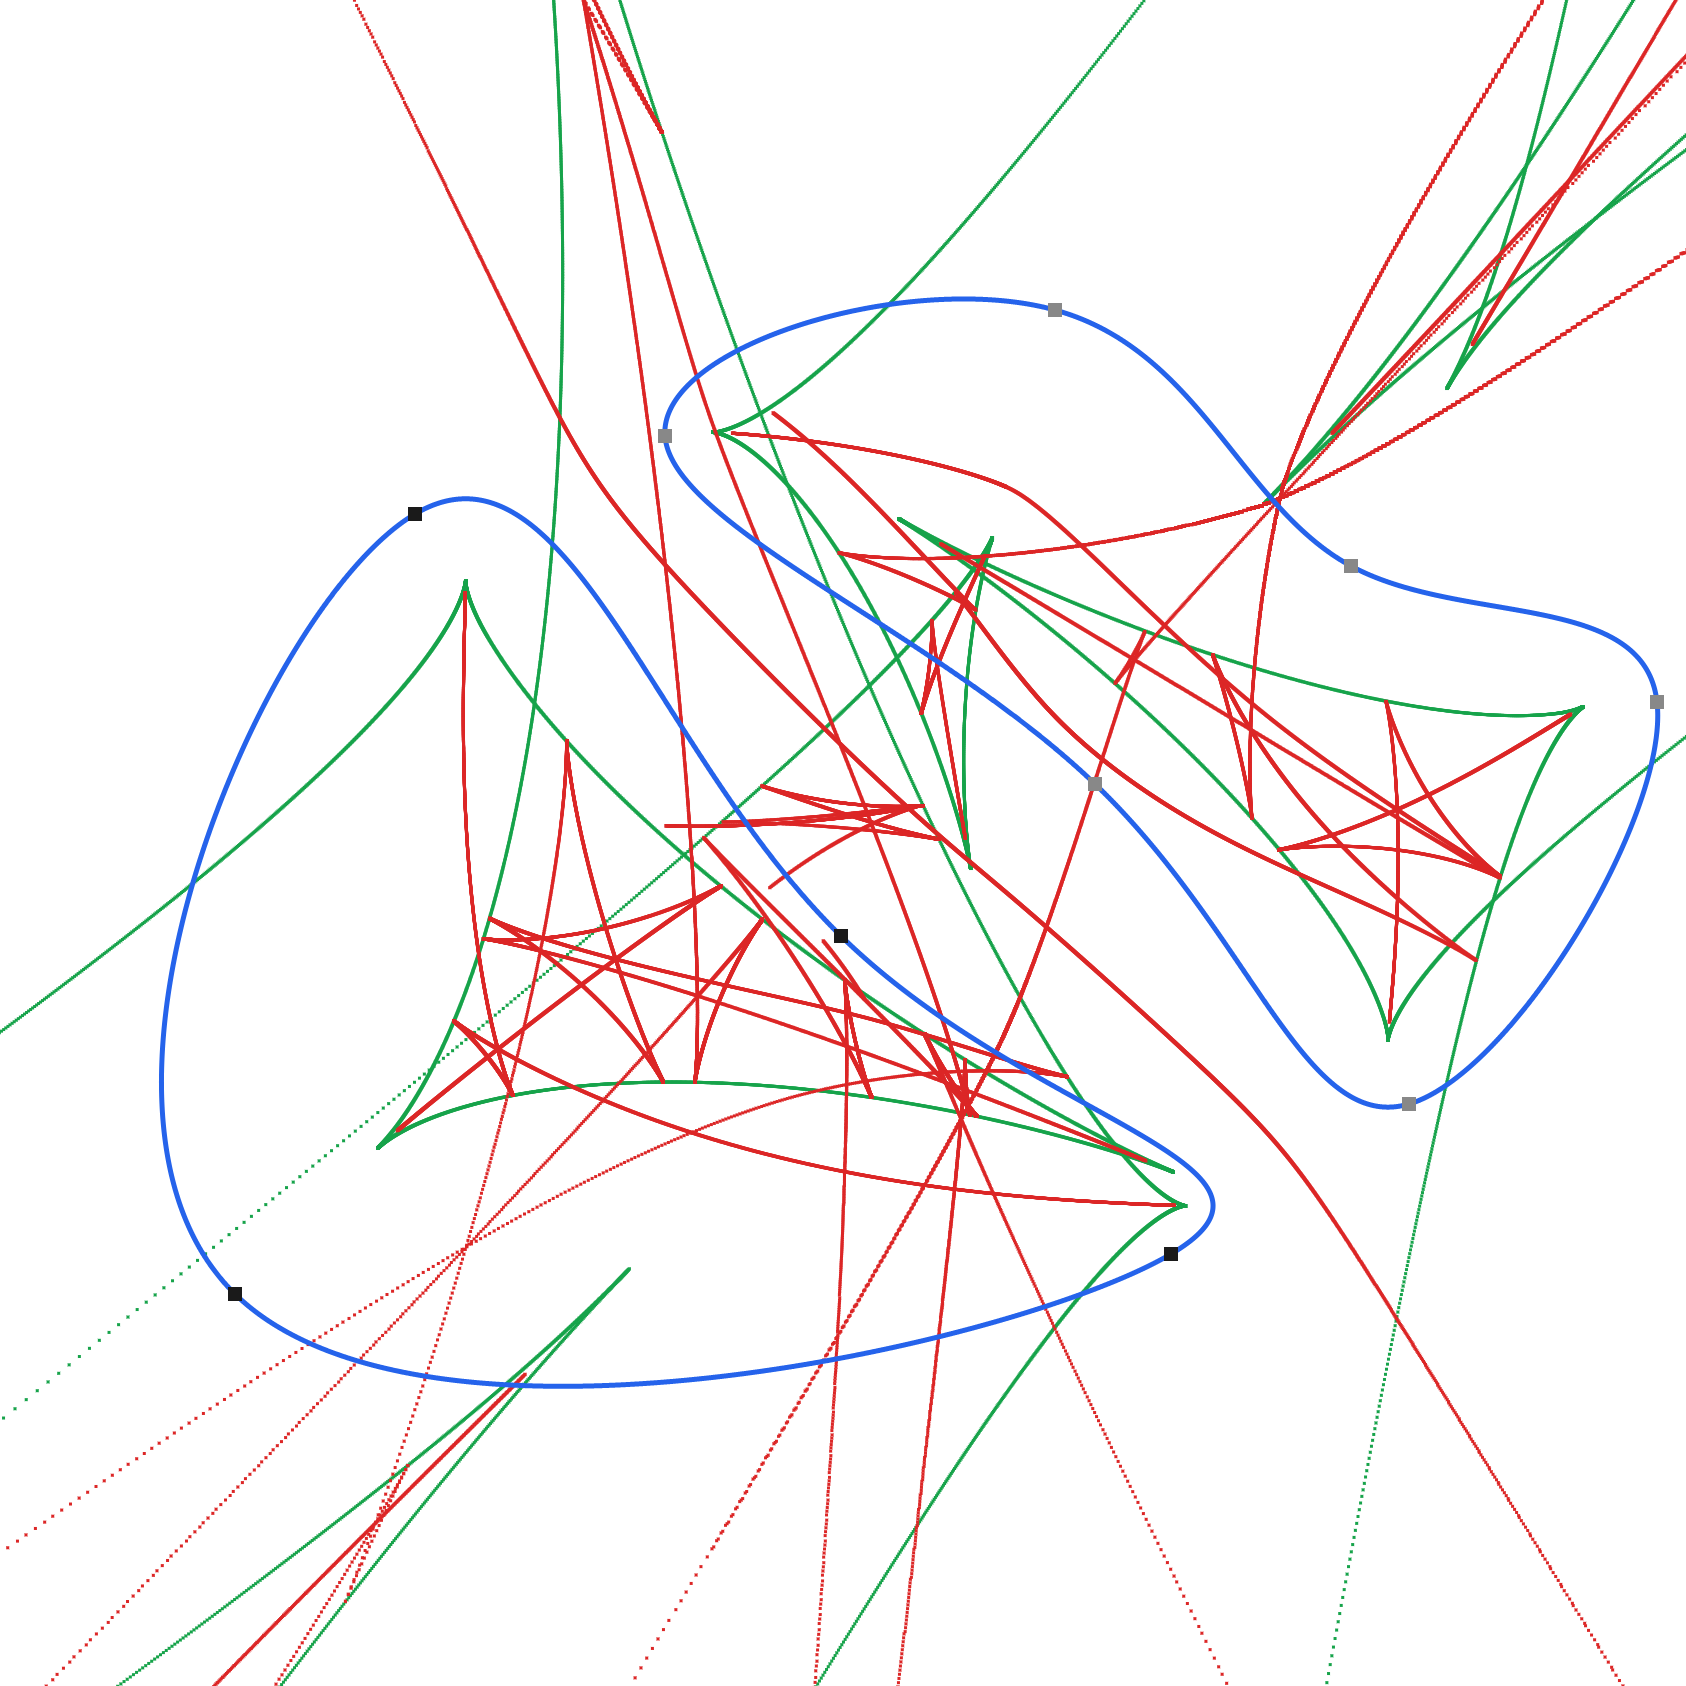
\includegraphics[width=0.47\linewidth]{figures/2_components.png}}
    \caption{Complex symmetry and focal sets arising from arbitrary spline curves. The figure on the bottom right captures the symmetry and focal sets arising from 2 connected components.}
    \label{fig:fun_pics}
\end{figure}

\subsection{Vineyards and Singularity Crossings}
Finally, we examine the stability of the Radial Persistence Transform by computing the vineyard along a circular loop $\gamma$ (shown in purple). Figure \ref{fig:vineyard_crossing} explicitly visualizes that topological changes in the distance function occur precisely when the center of measurement crosses the focal set.

In the top row of Figure \ref{fig:vineyard_crossing}, the yellow center point traverses a region free of focal singularities, and the corresponding vine (blue curve in the 3D plot) remains continuous. As the center crosses the green focal curve (middle and bottom rows), we observe a distinct ``break'' or discontinuity in the vineyard. 
% This visual discontinuity confirms the change in the number or pairing of critical points.
Figure \ref{fig:vin_change} further explores this by varying the radius of the loop $\gamma$, showing how the vines evolve as the measurement loop encompasses different topological features of the ambient space.

\begin{figure}[htbp]
    \centering
    % Each image is scaled to slightly less than 33% to account for spacing
    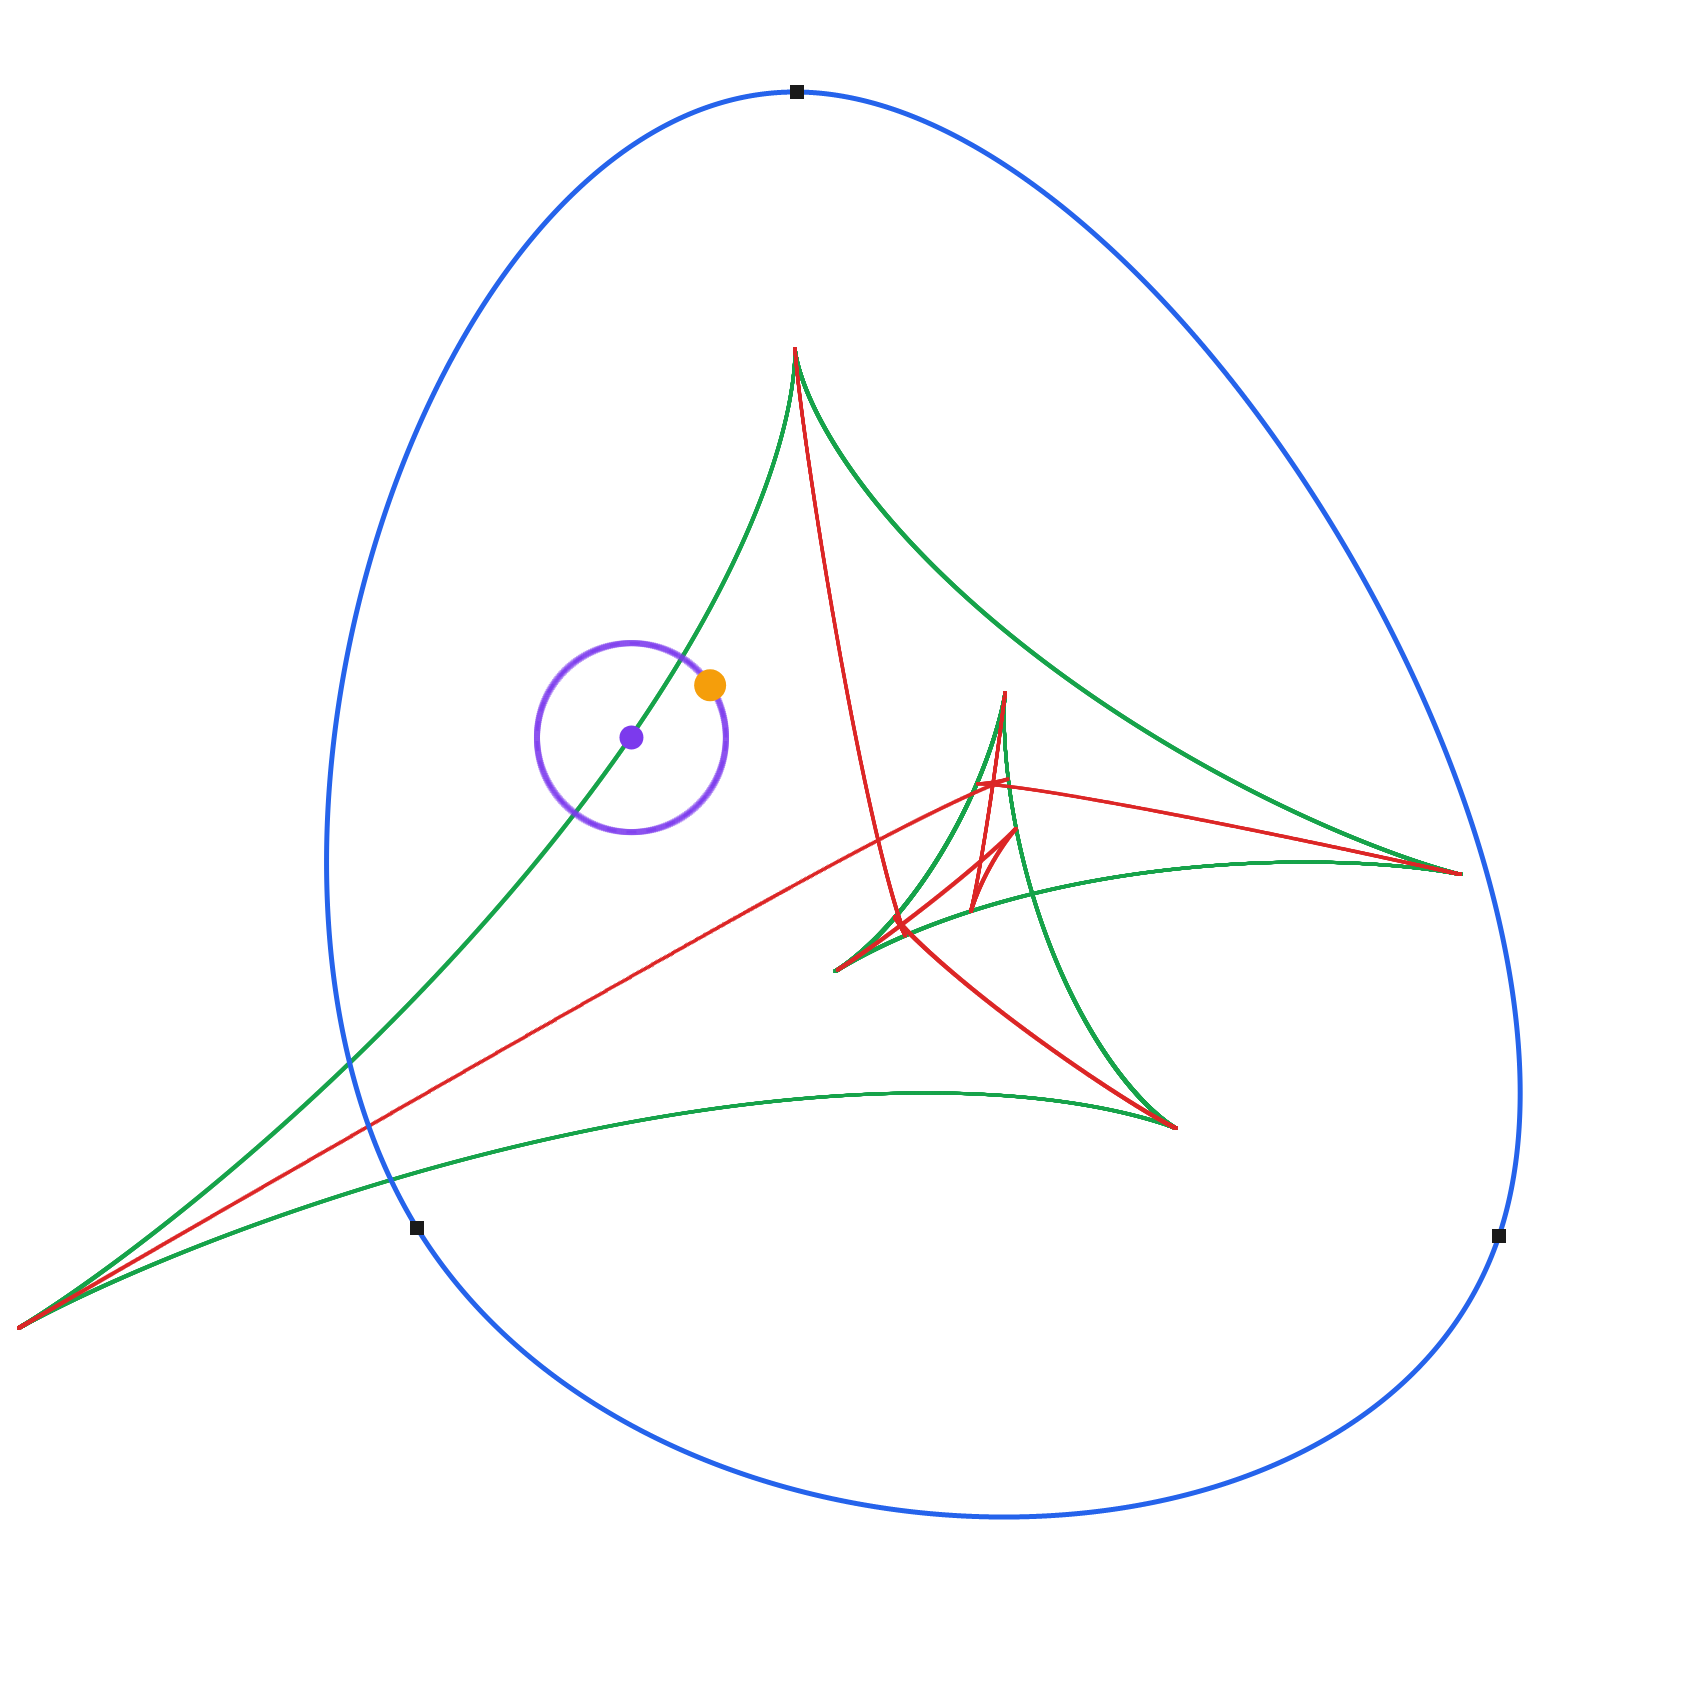
\includegraphics[width=0.32\textwidth]{canvas1.png}
    \hfill
    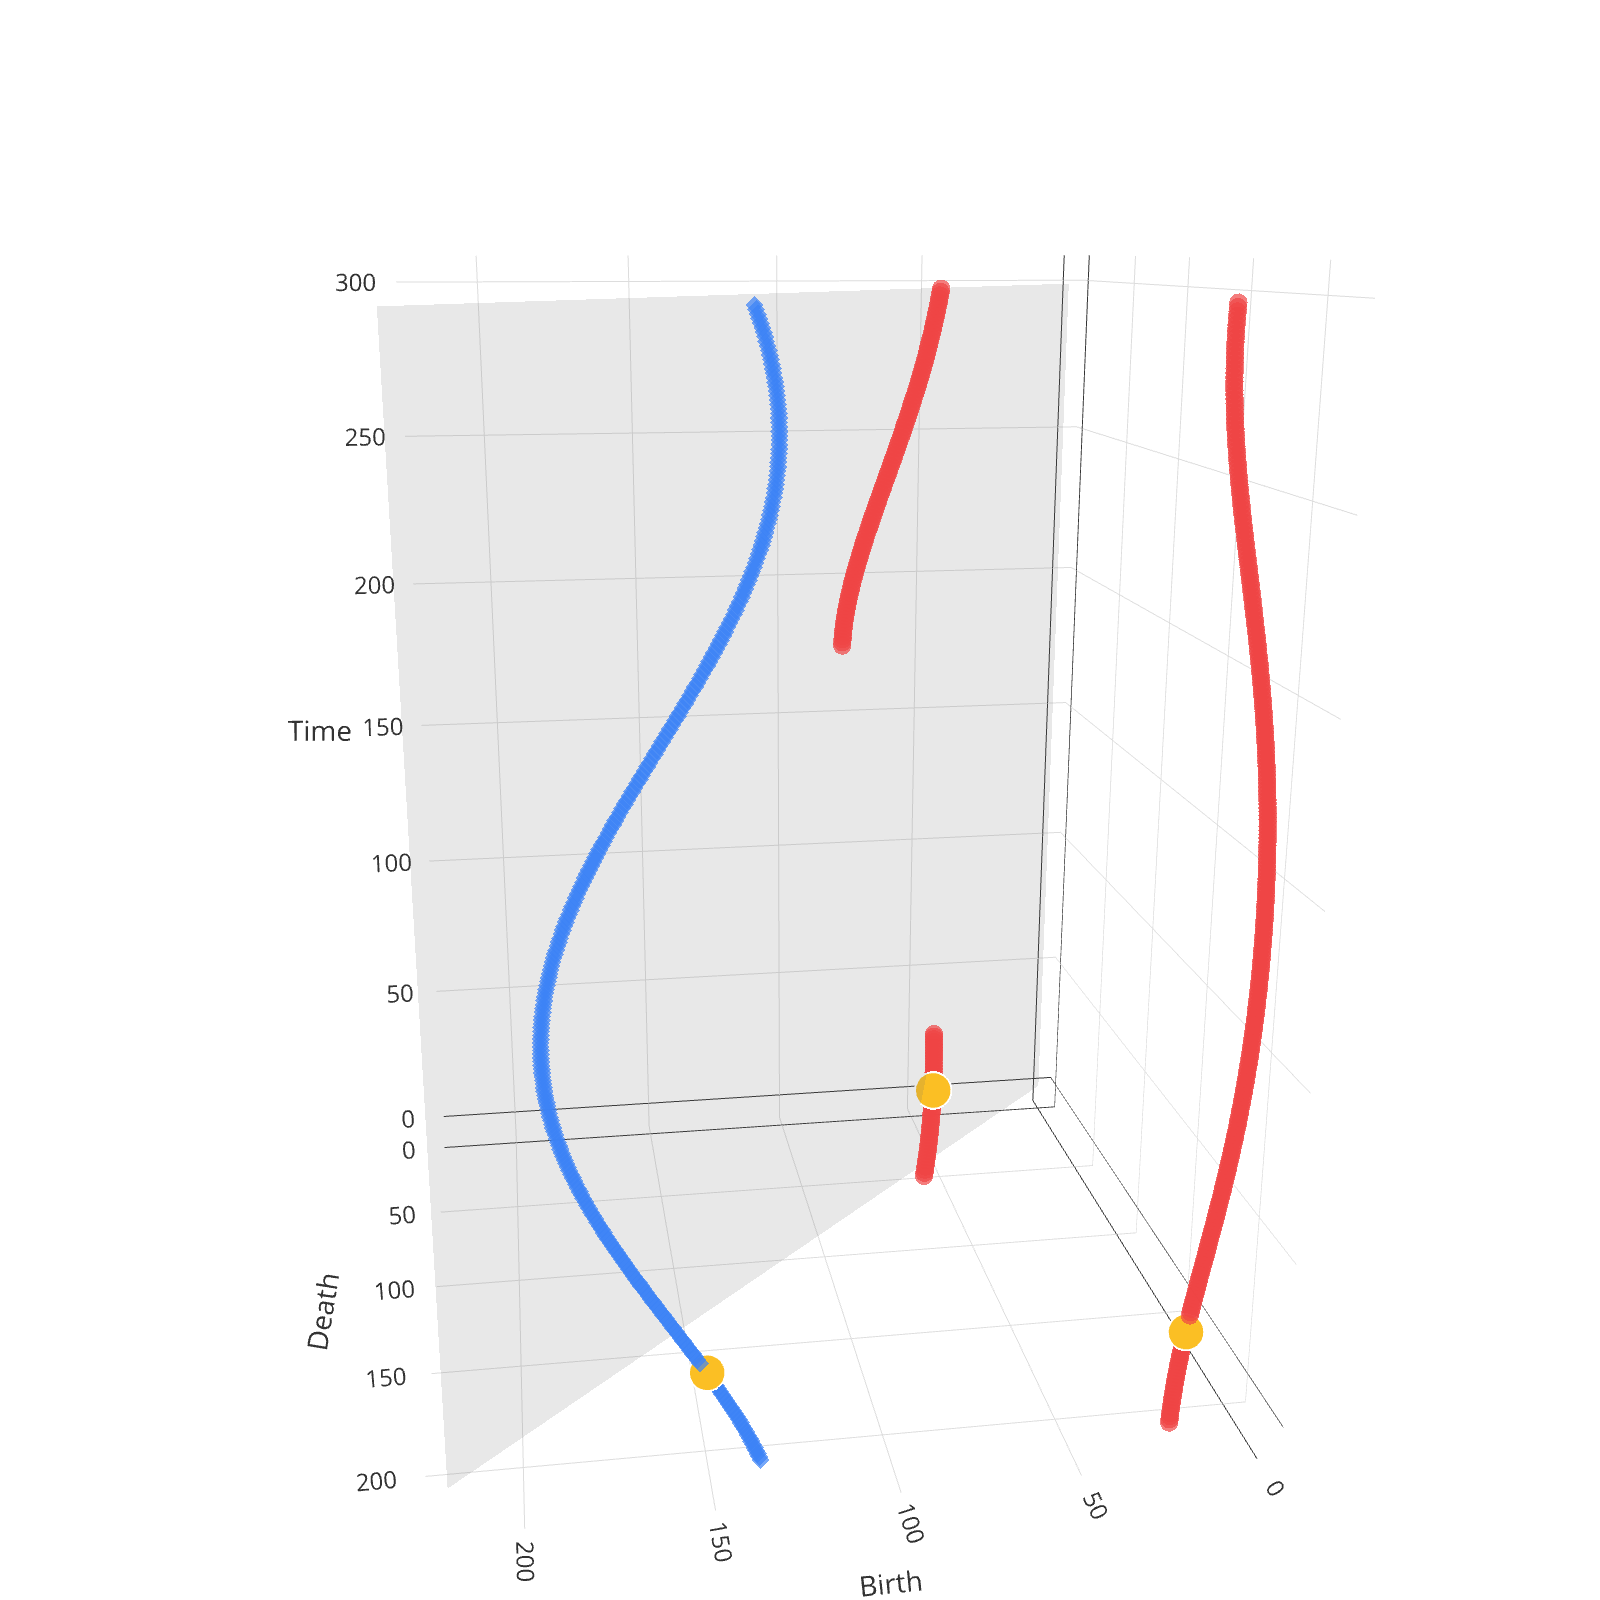
\includegraphics[width=0.36\textwidth]{vin1.png}
    \hfill
    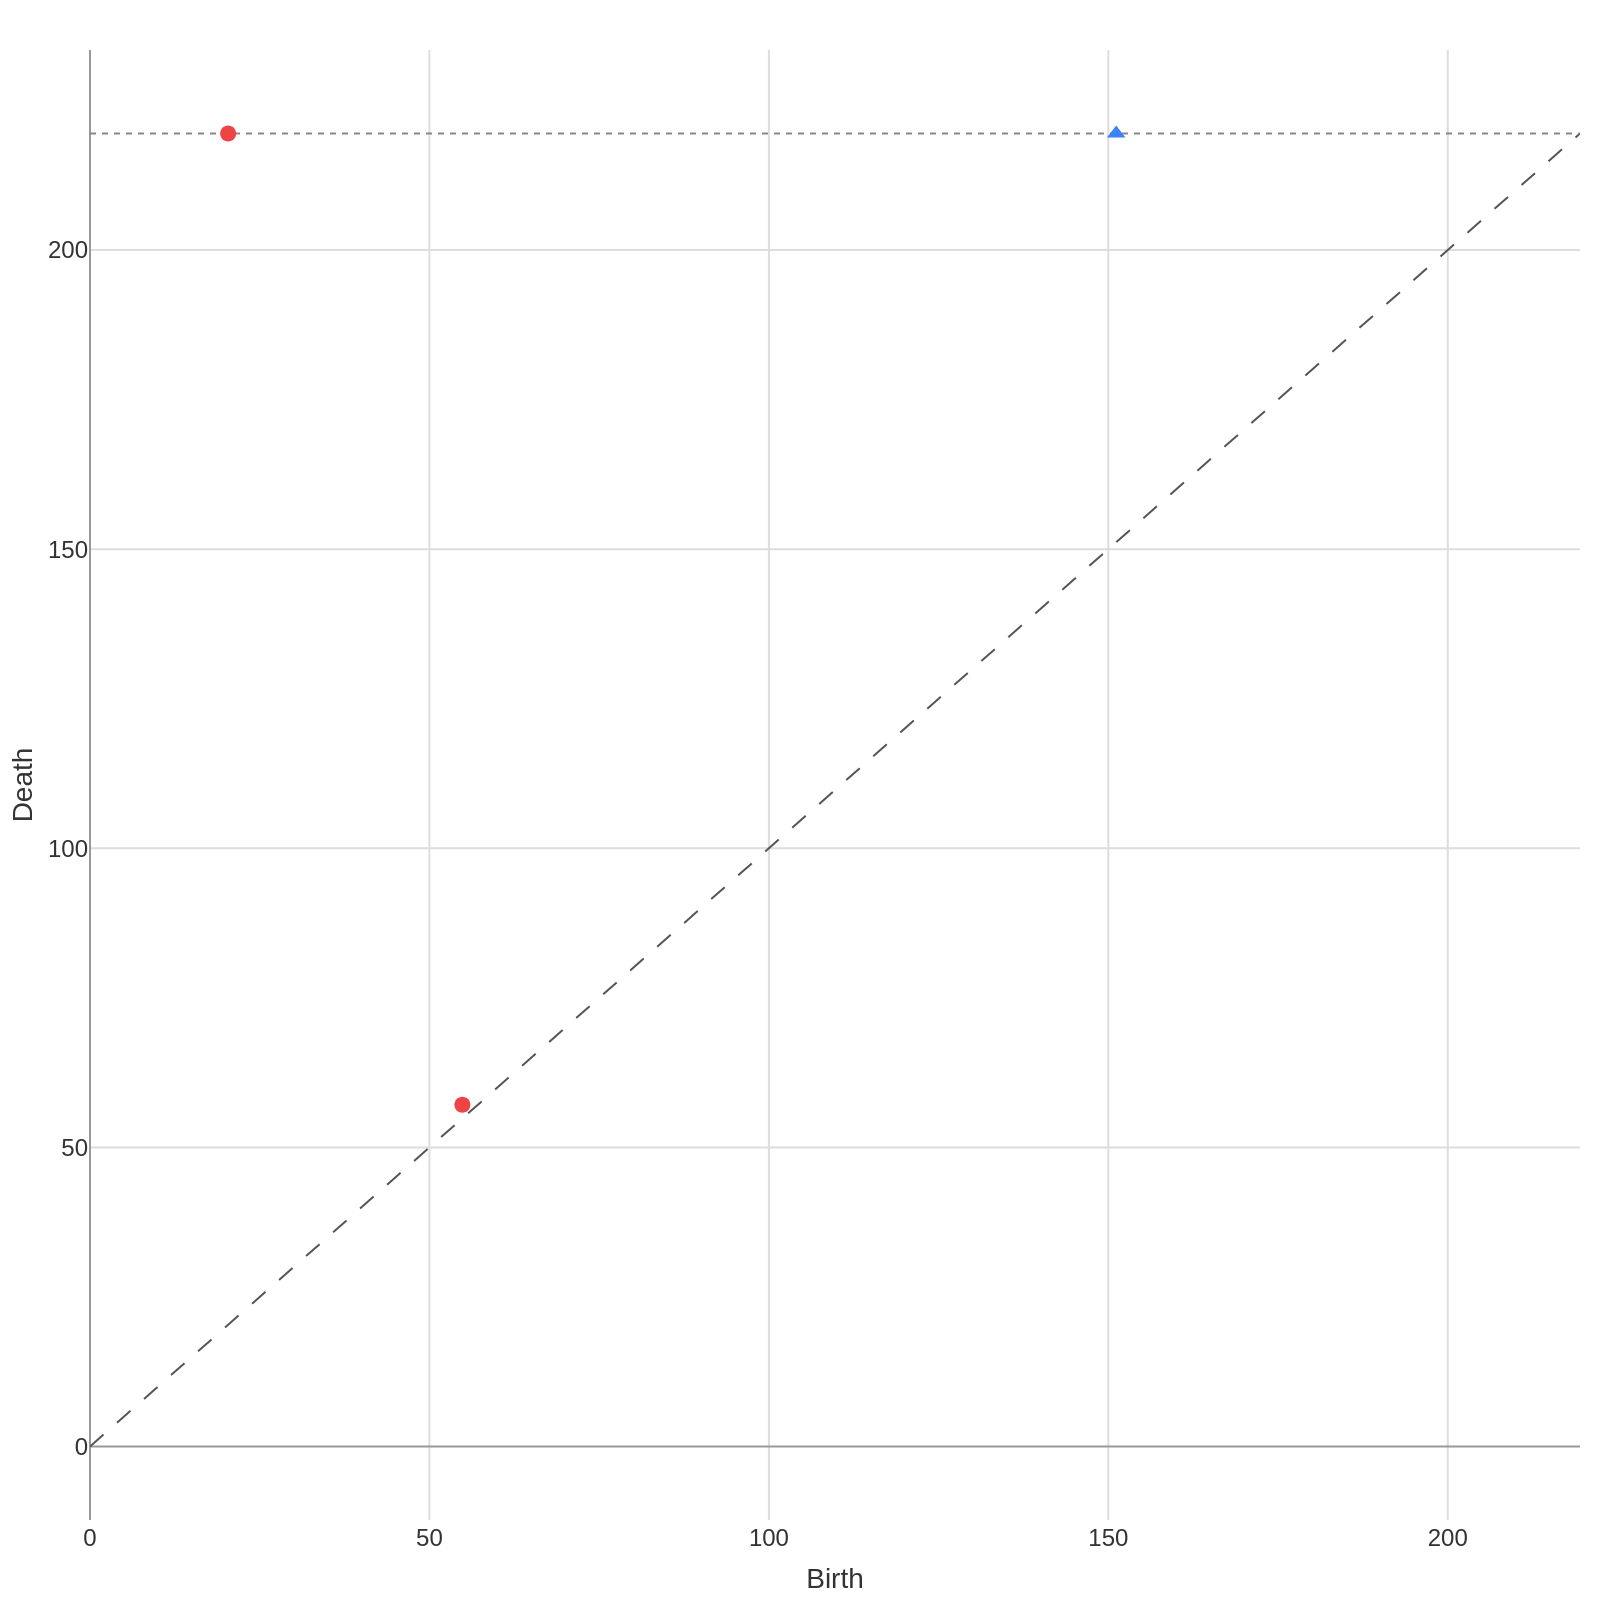
\includegraphics[width=0.29\textwidth]{persistence_diagram1.png}

    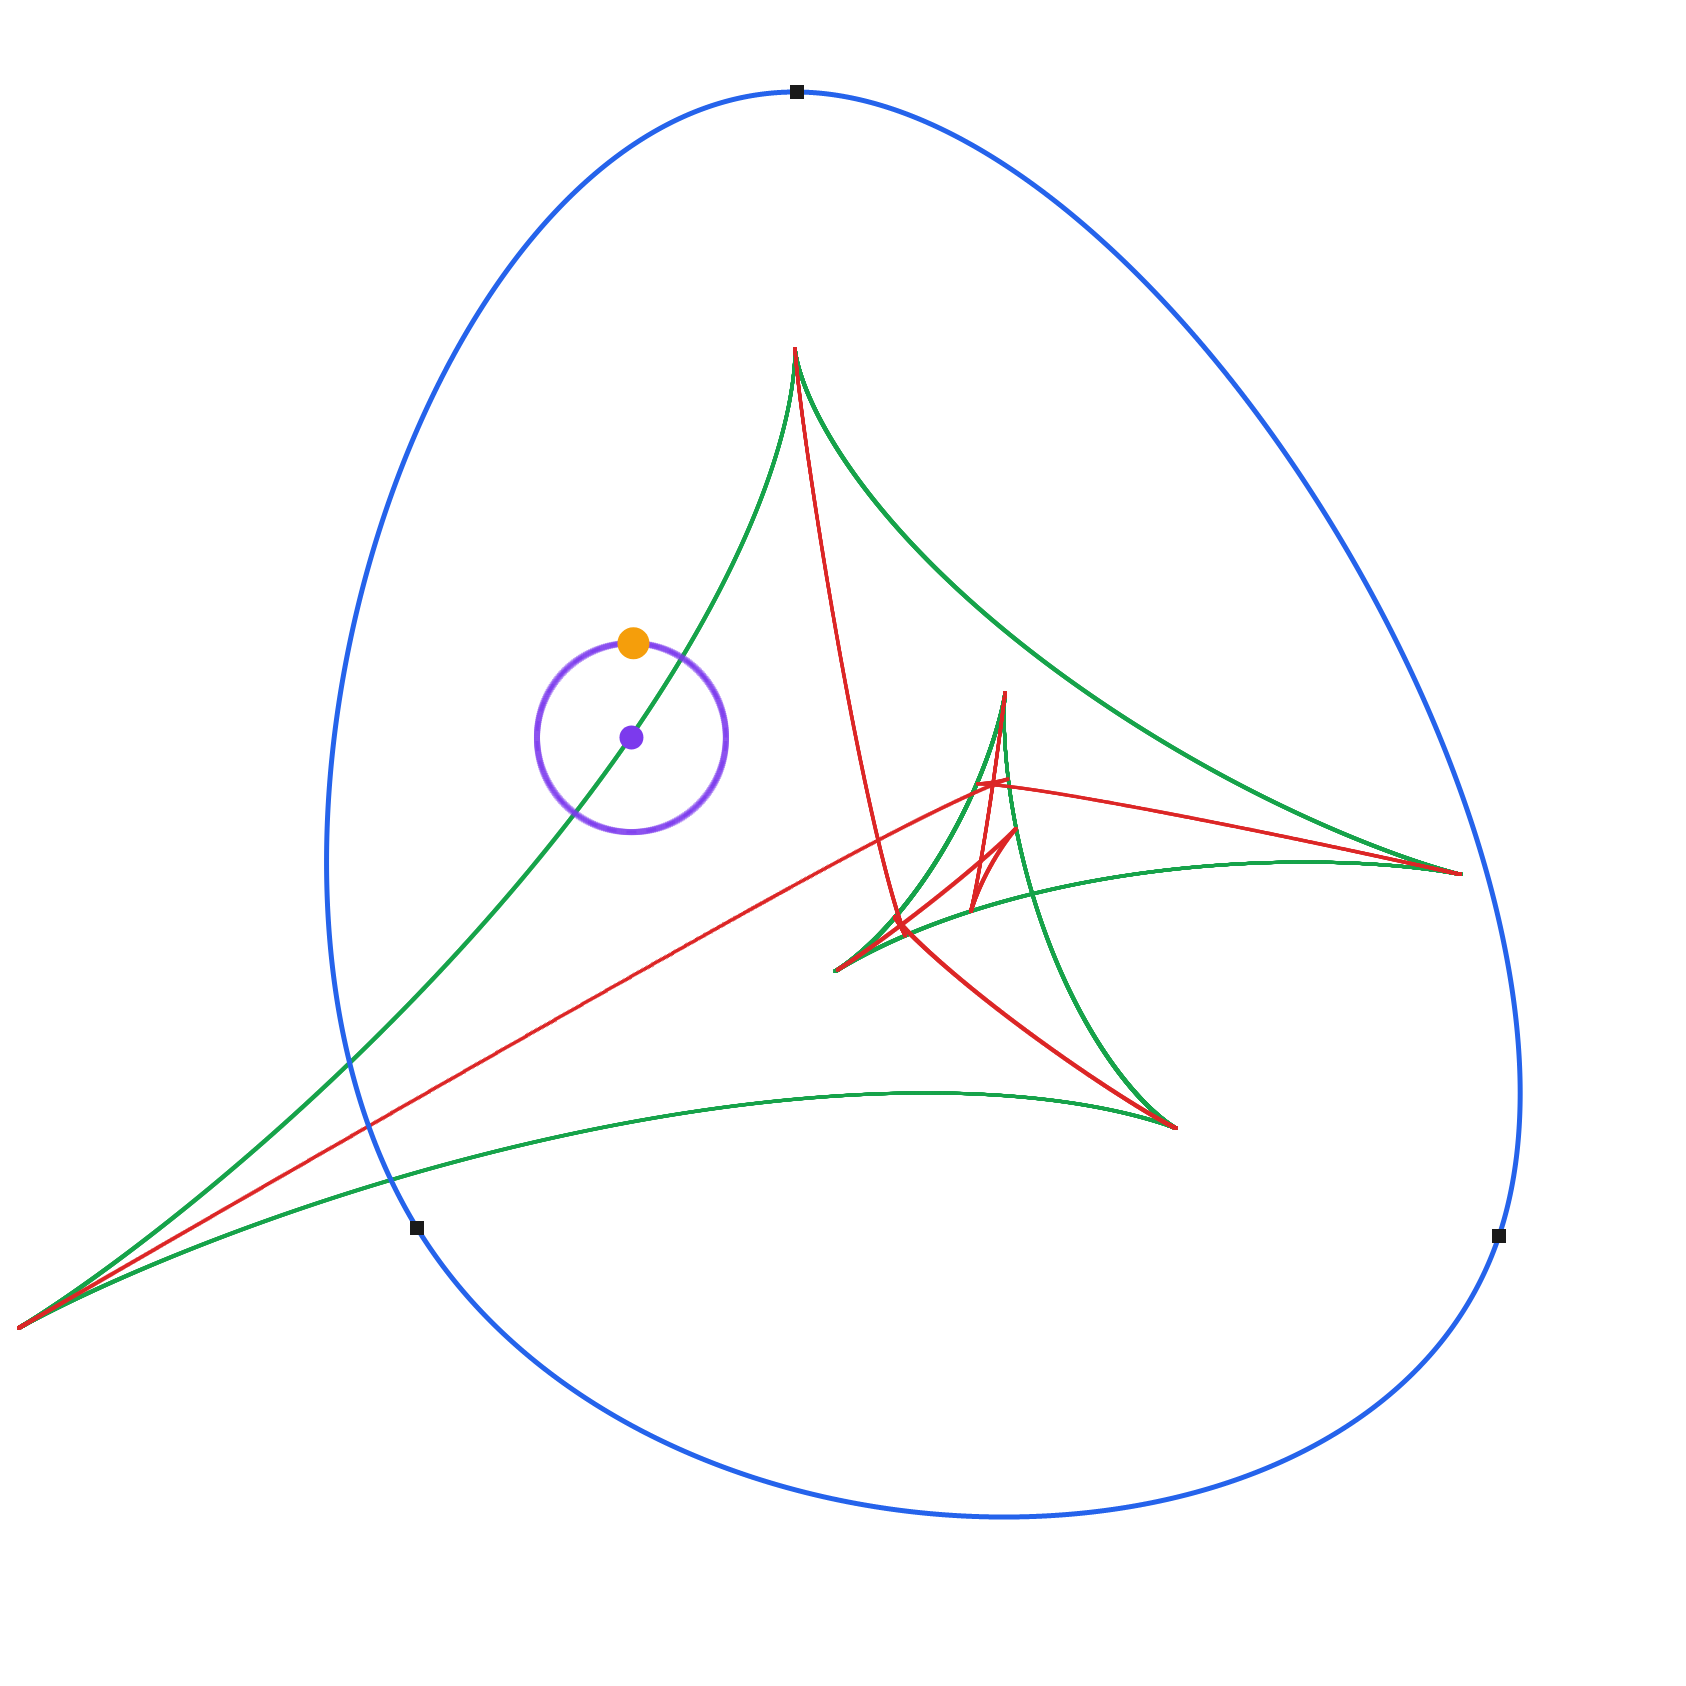
\includegraphics[width=0.32\textwidth]{canvas2.png}
    \hfill
    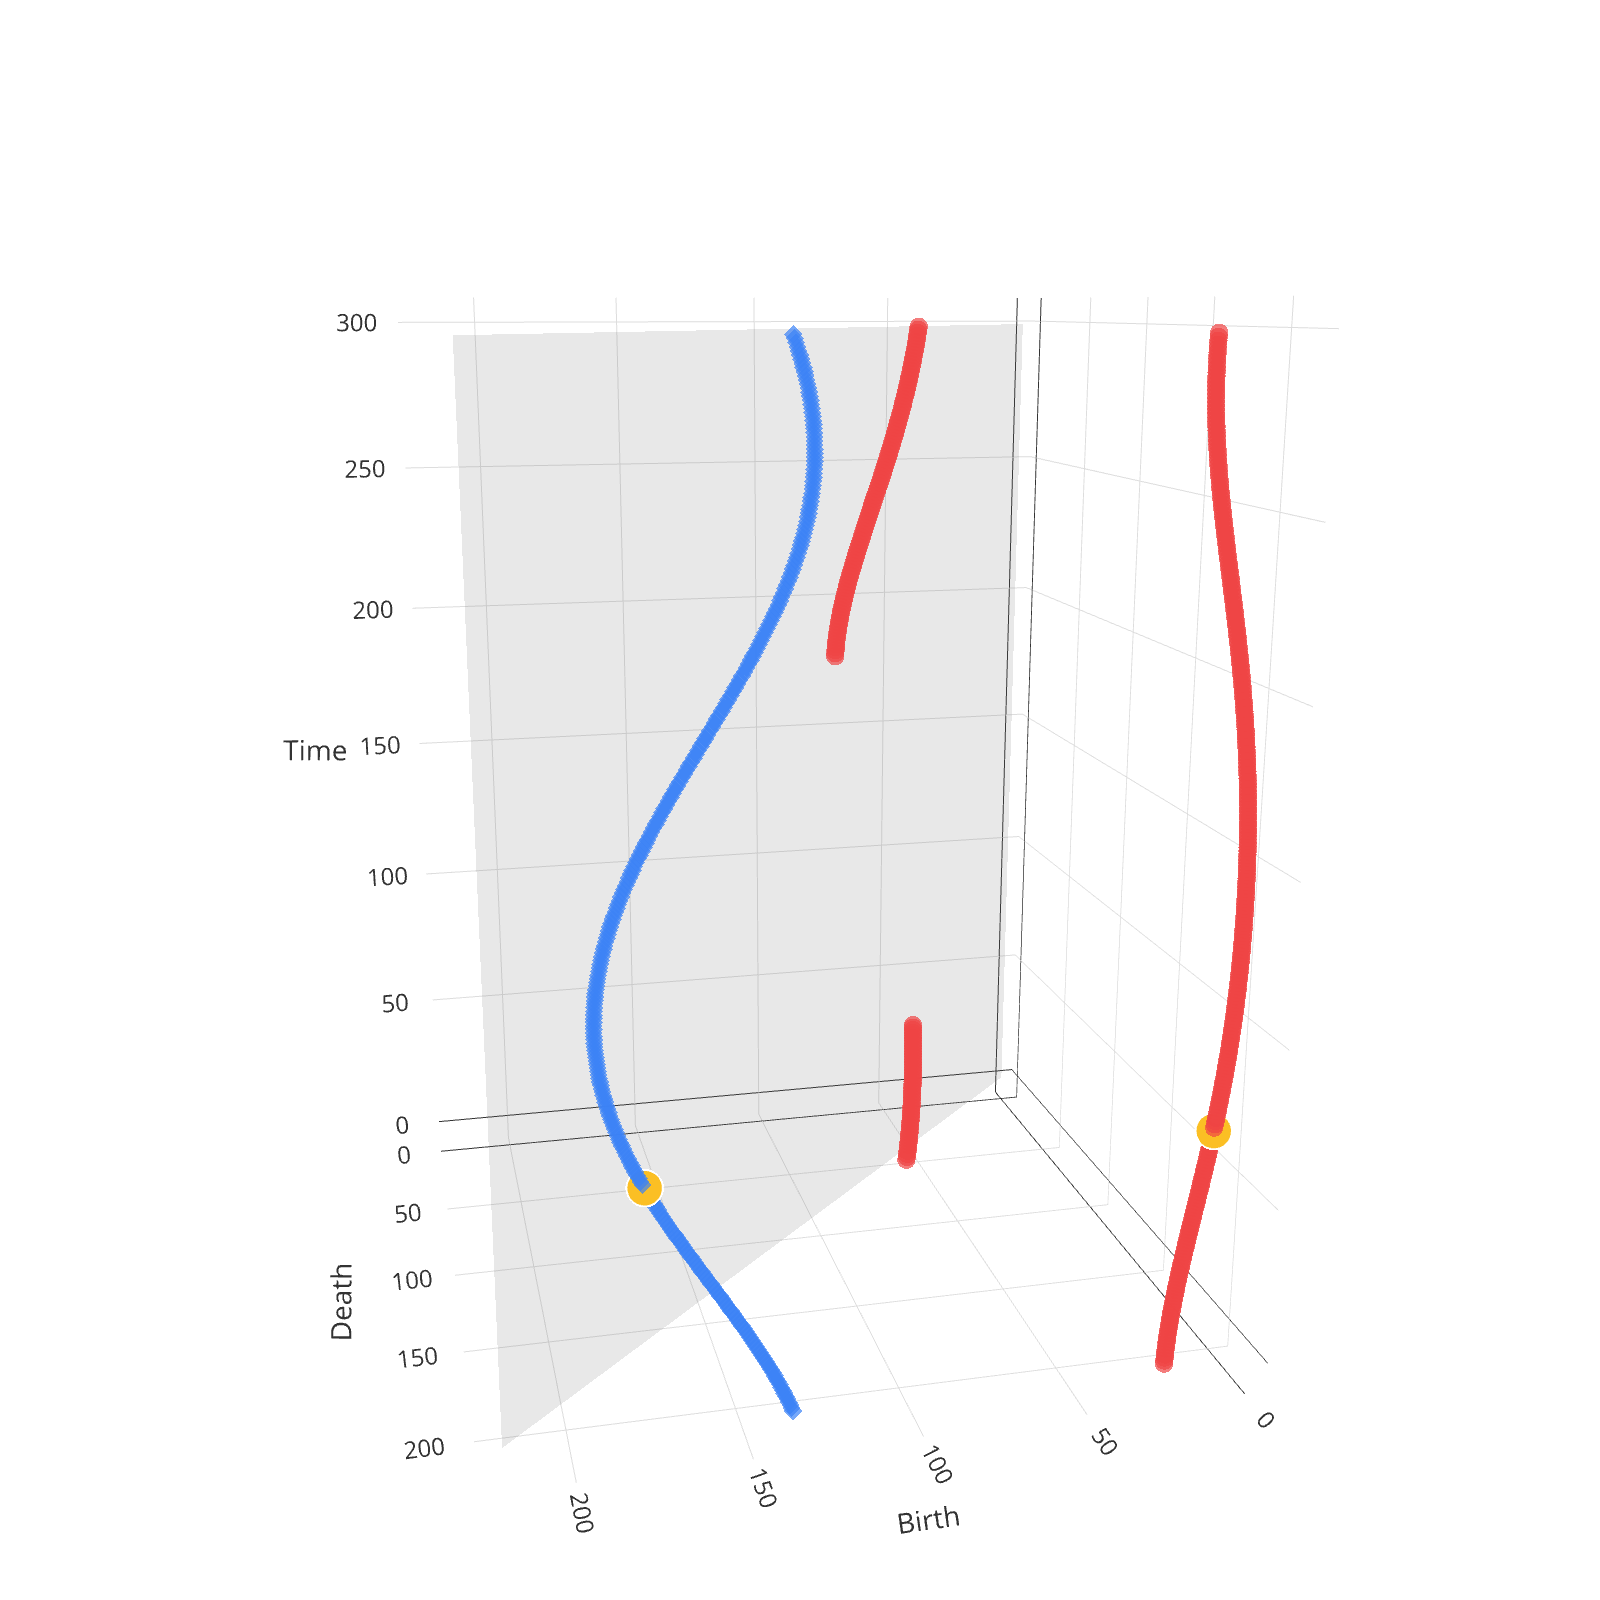
\includegraphics[width=0.36\textwidth]{vin2.png}
    \hfill
    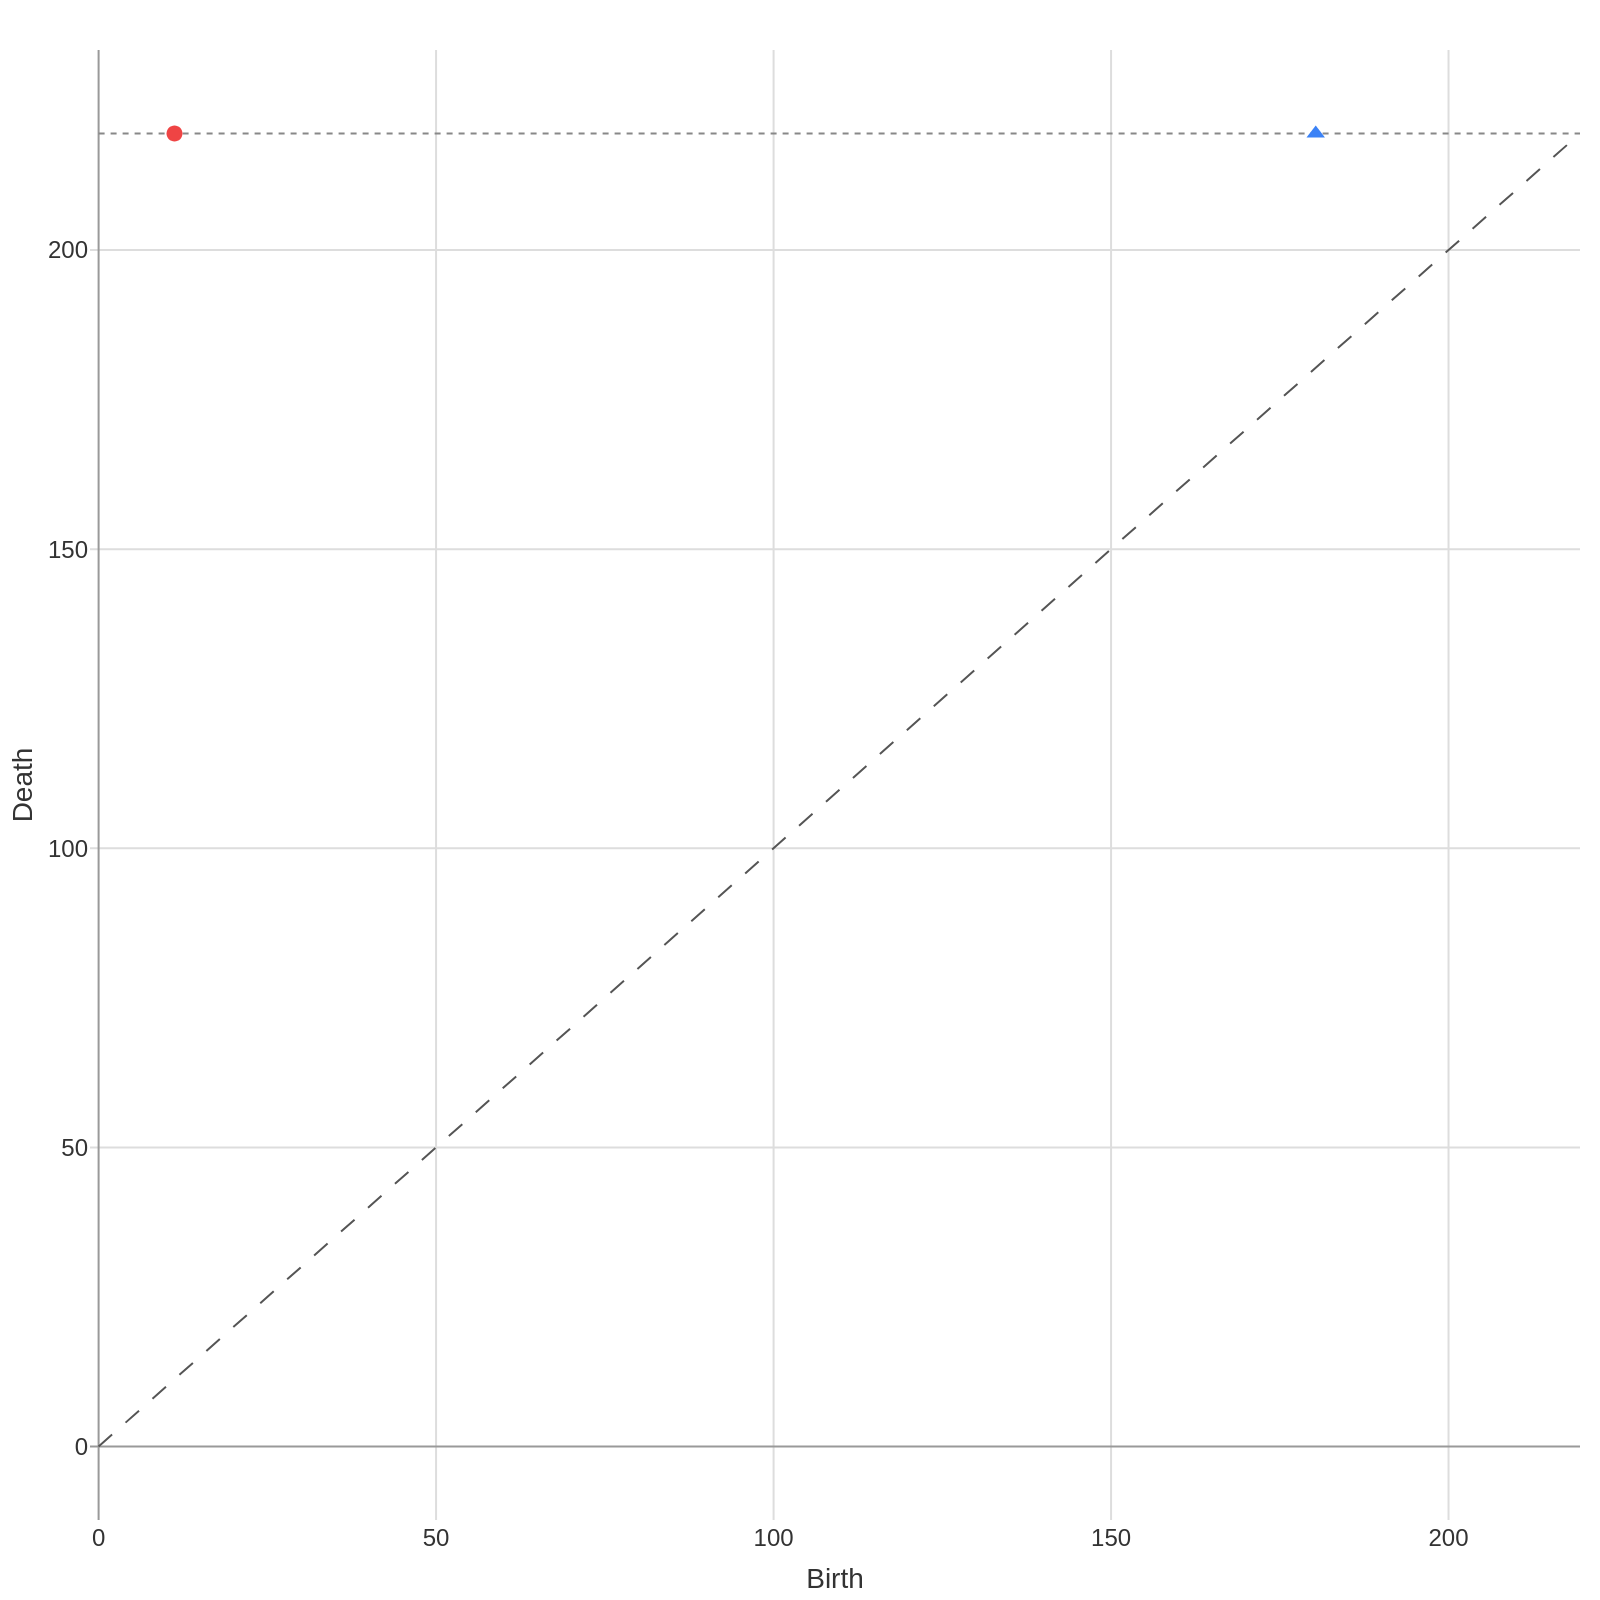
\includegraphics[width=0.29\textwidth]{persistence_diagram2.png}

    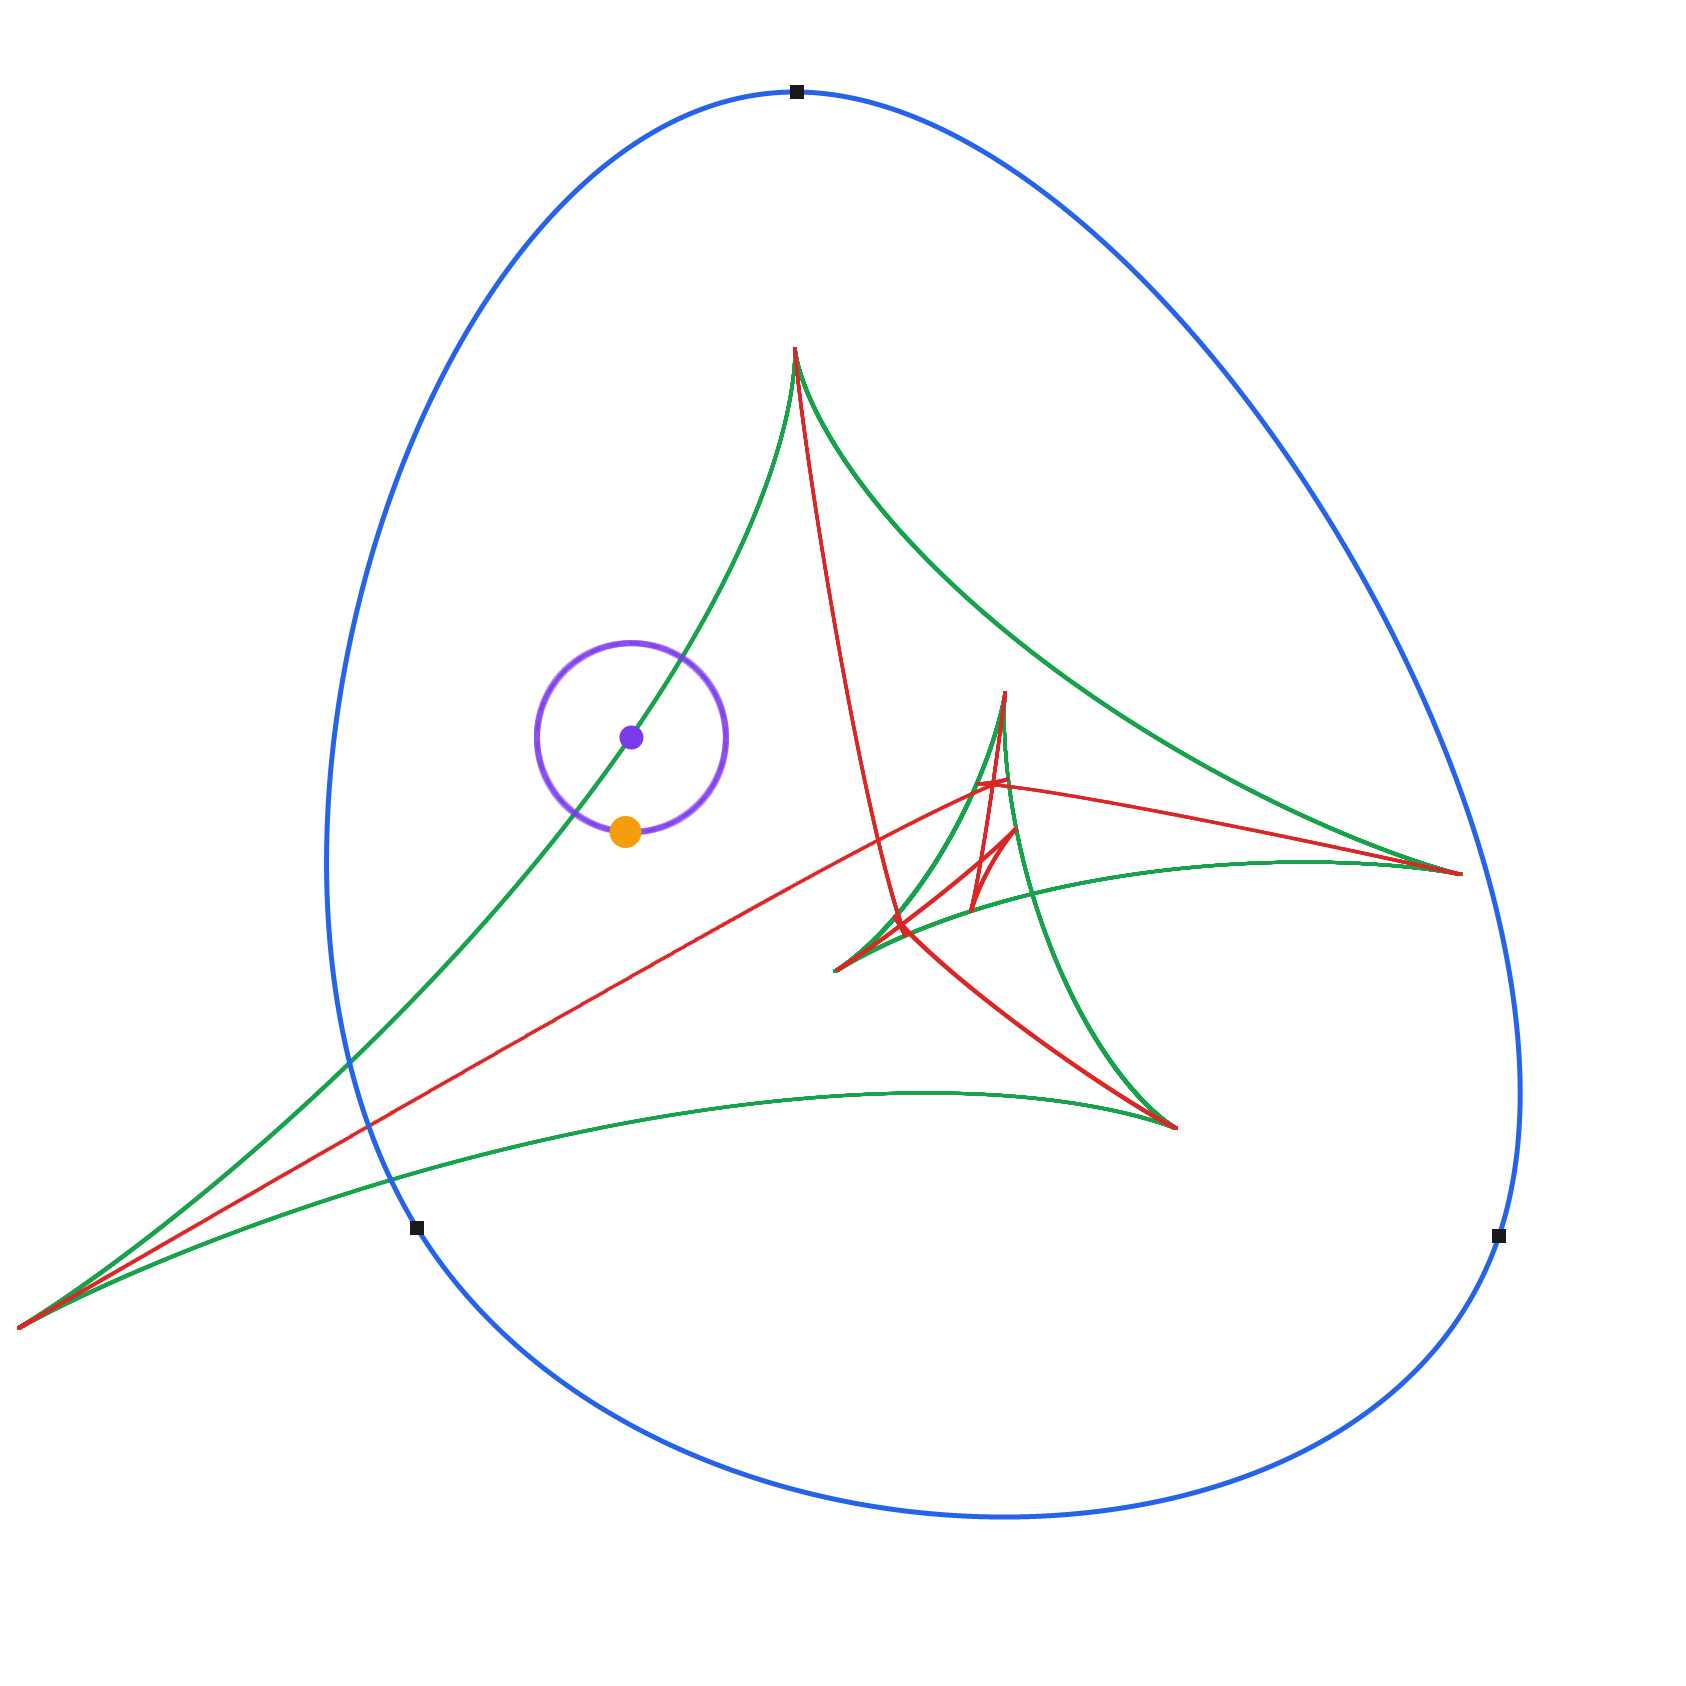
\includegraphics[width=0.32\textwidth]{canvas3.png}
    \hfill
    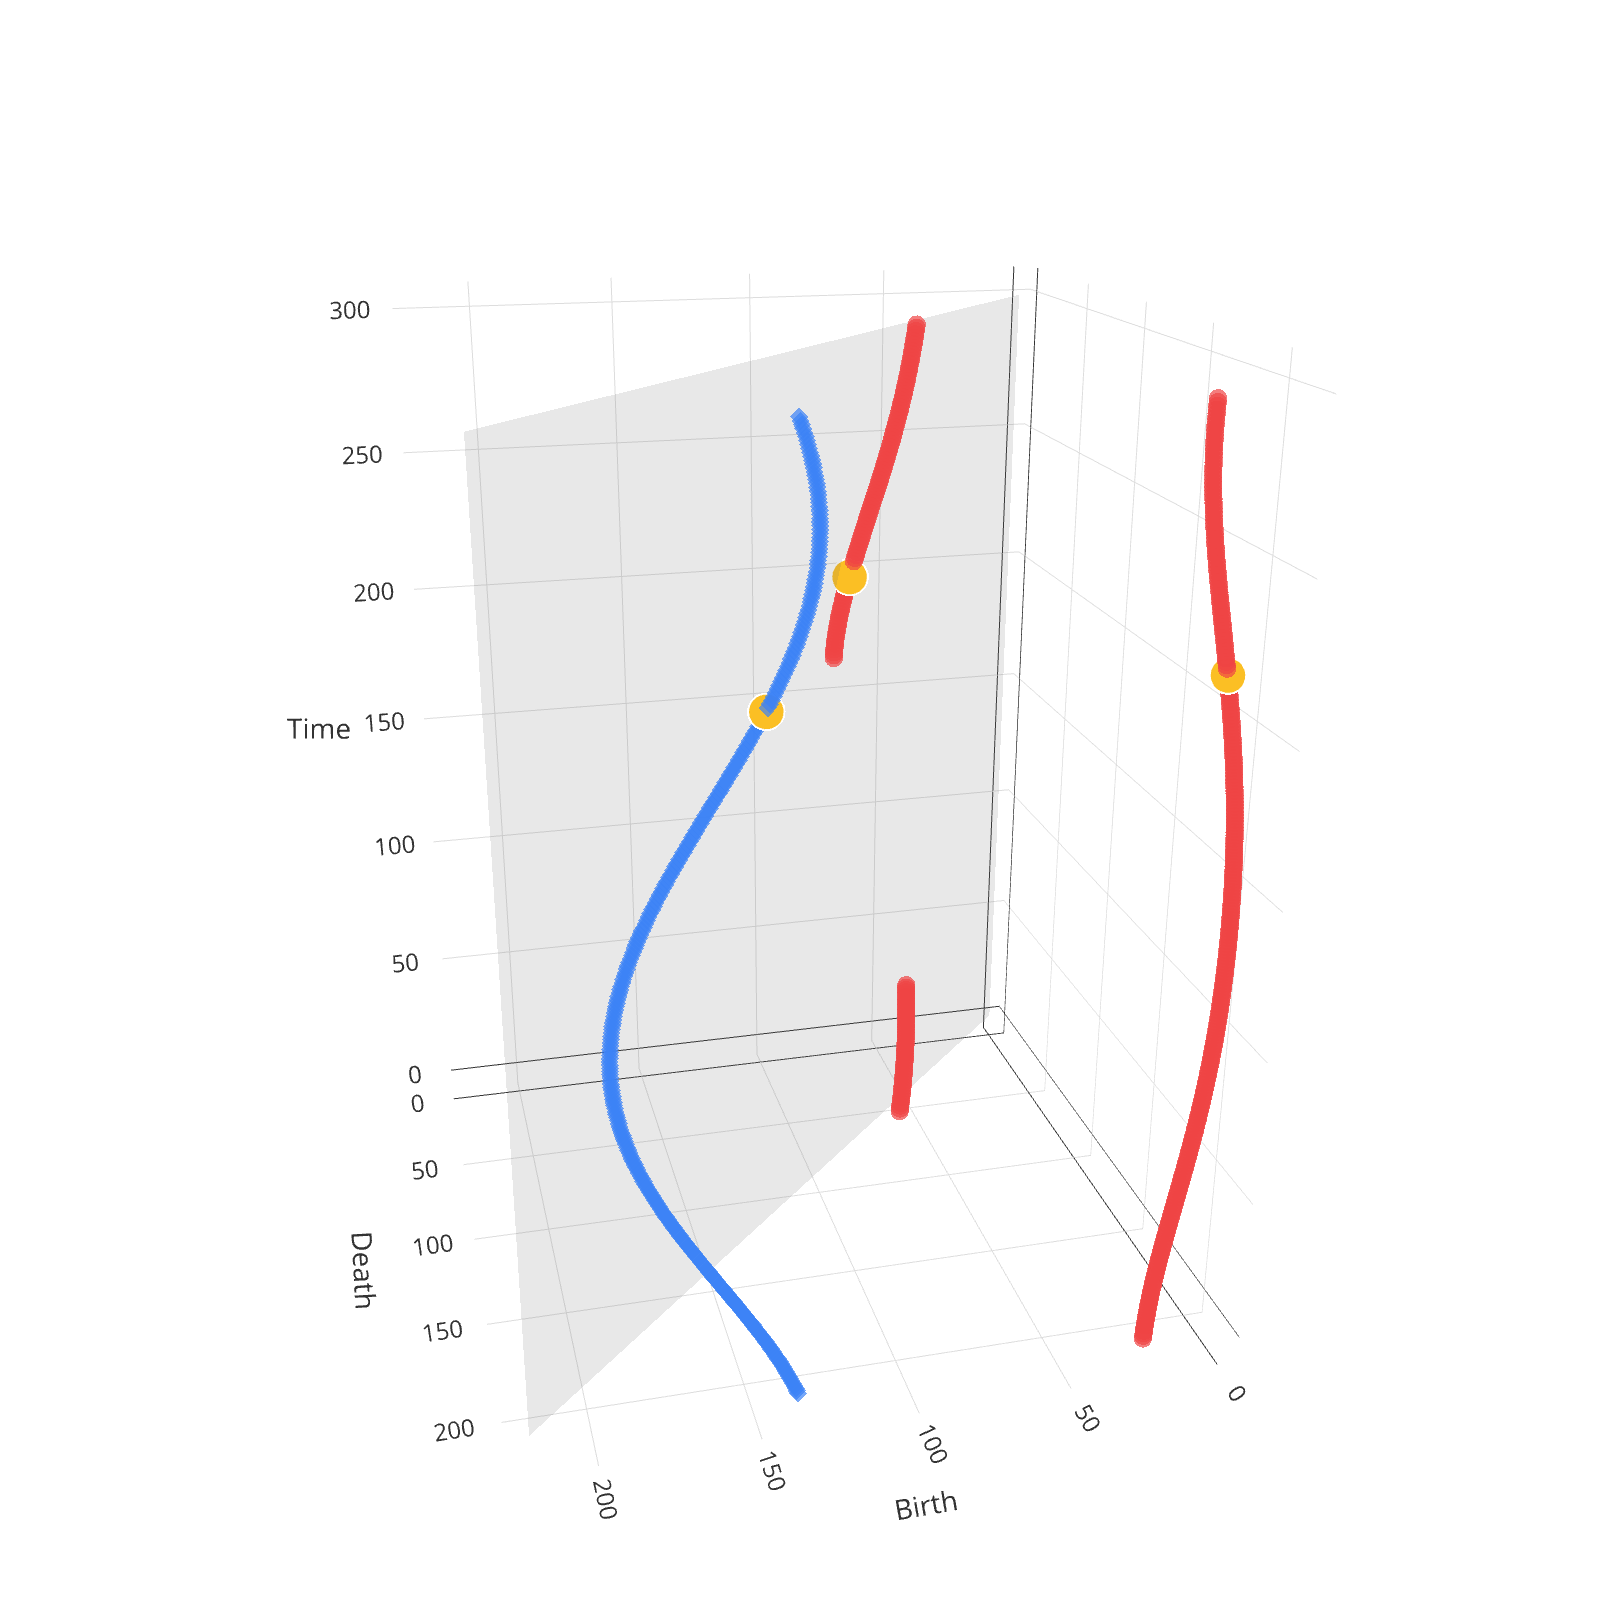
\includegraphics[width=0.36\textwidth]{vin3.png}
    \hfill
    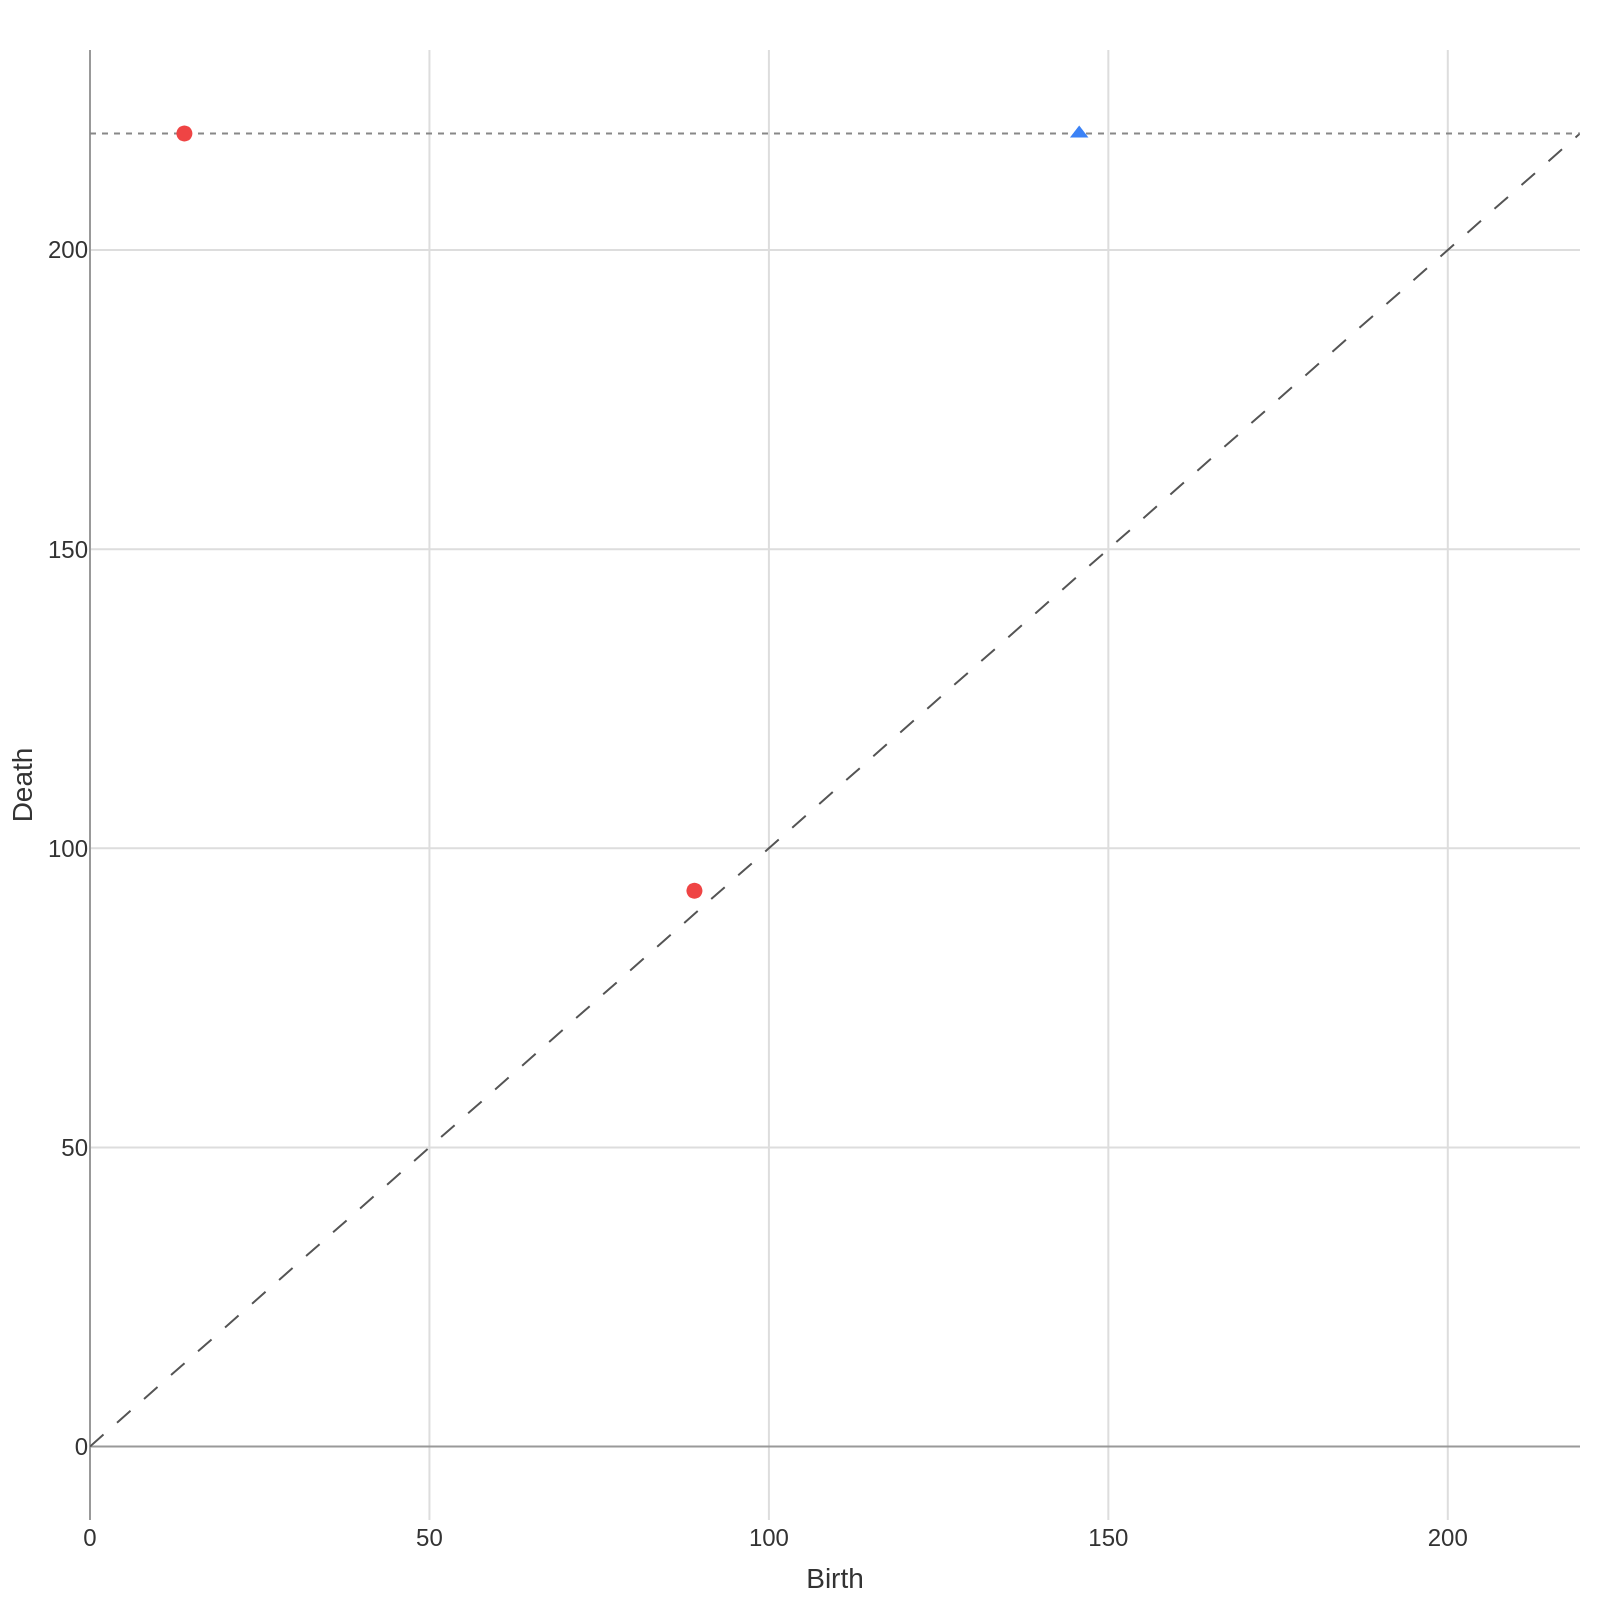
\includegraphics[width=0.29\textwidth]{persistence_diagram3.png}
    
    \caption{An example of a vineyard for a potato shaped figure along the purple loop. As the center (yellow point) crosses the focal set, there is a break in the vineyard, and when it crosses back again, the vineyard reappears.}
    \label{fig:vineyard_crossing}
\end{figure}

\begin{figure}
    \centering
    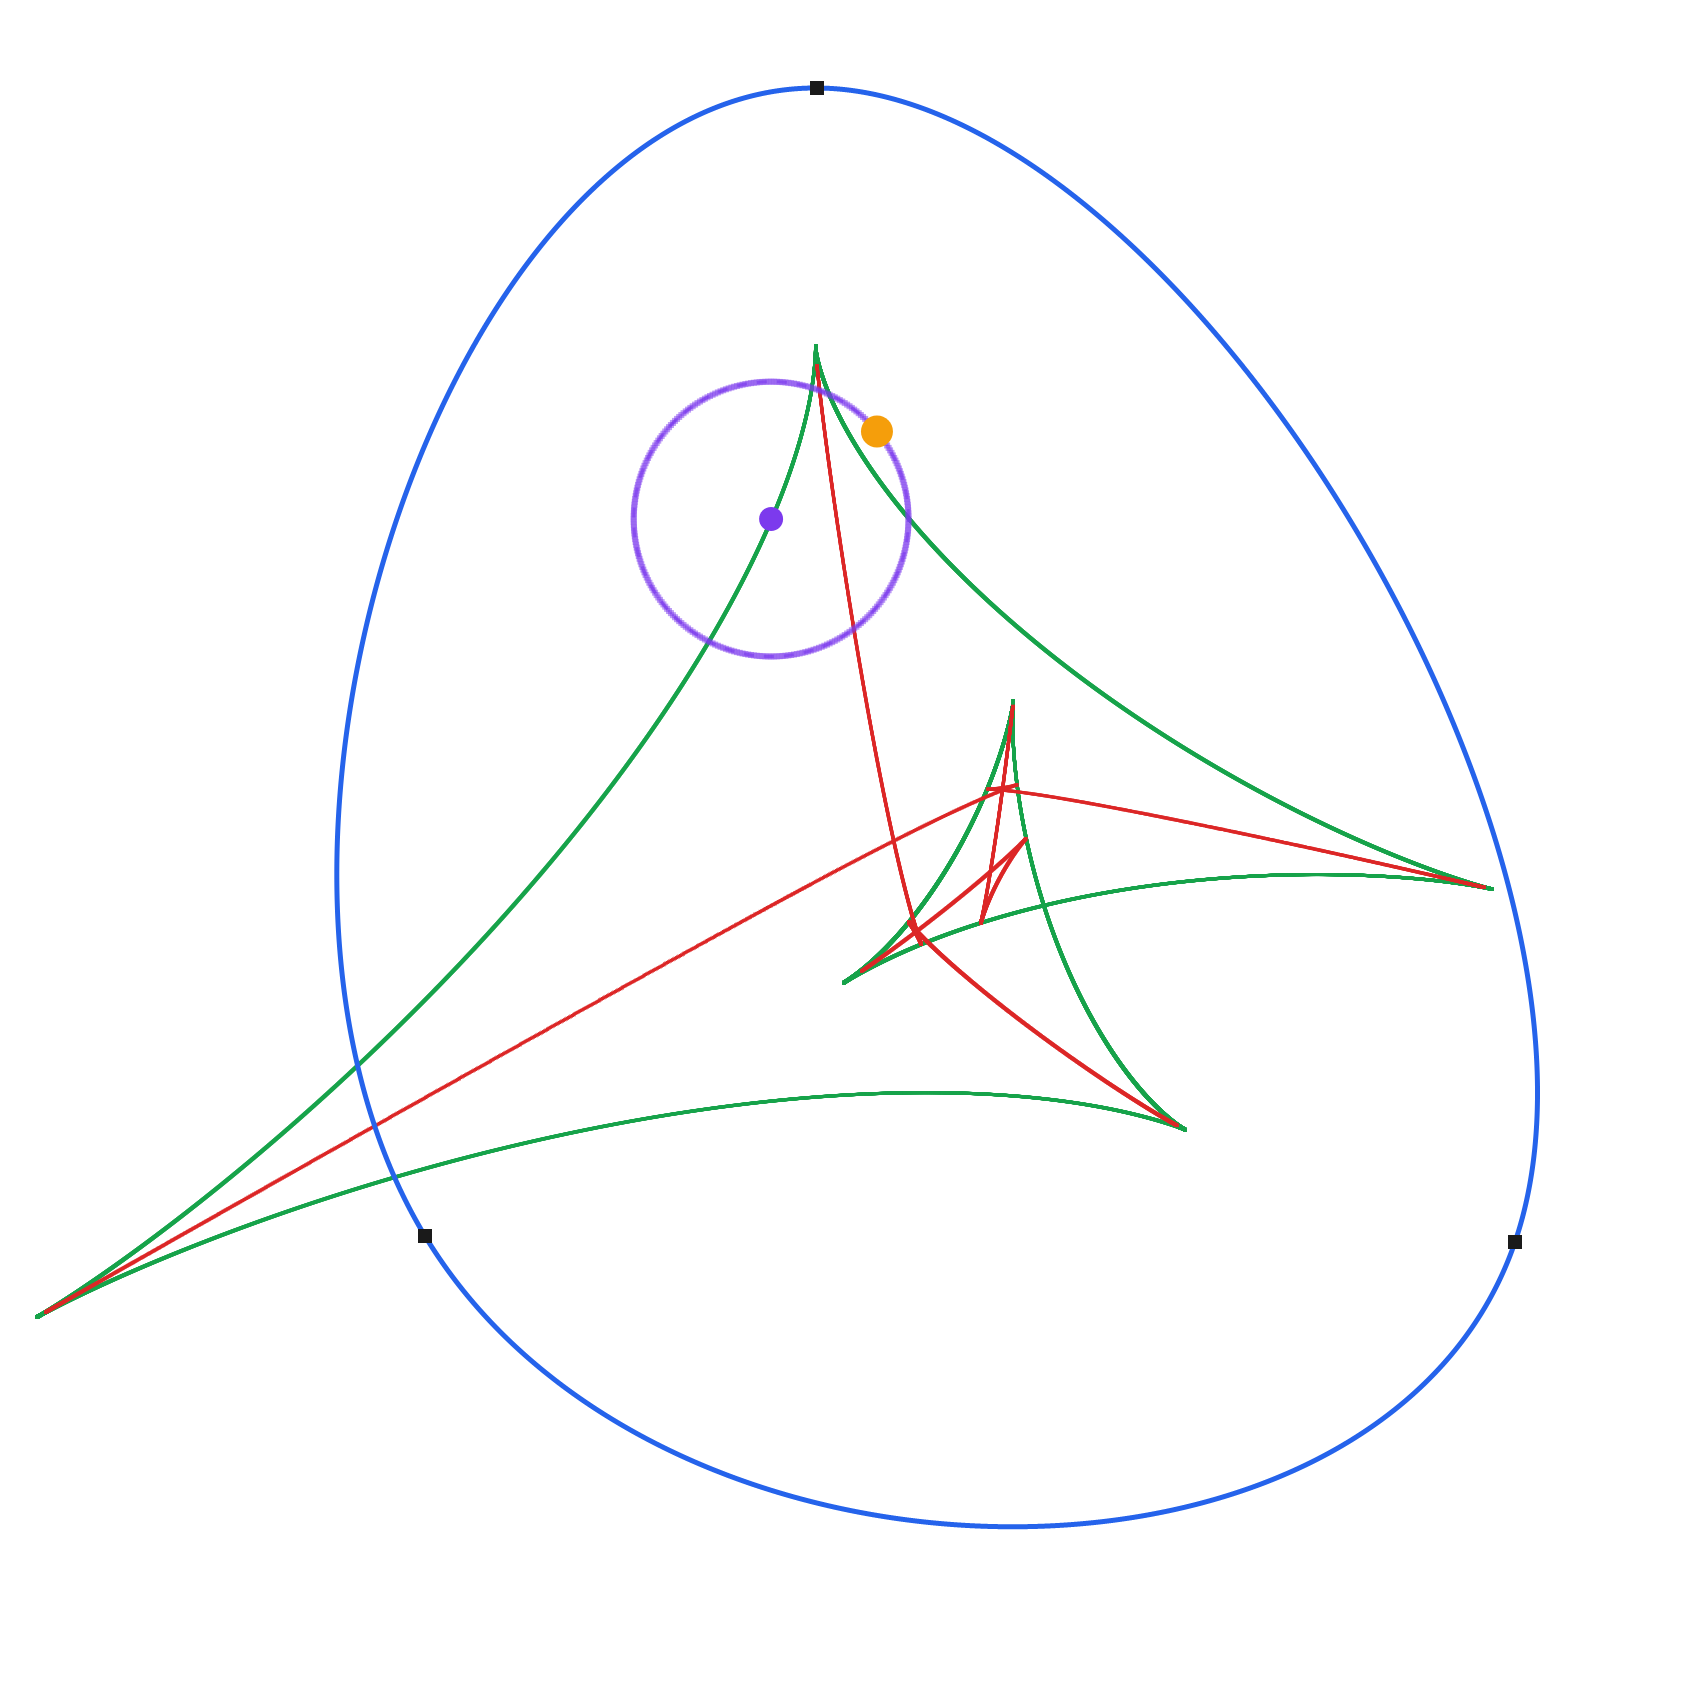
\includegraphics[width=0.47\linewidth]{figures/canvas_r1.png}
    \hfill
    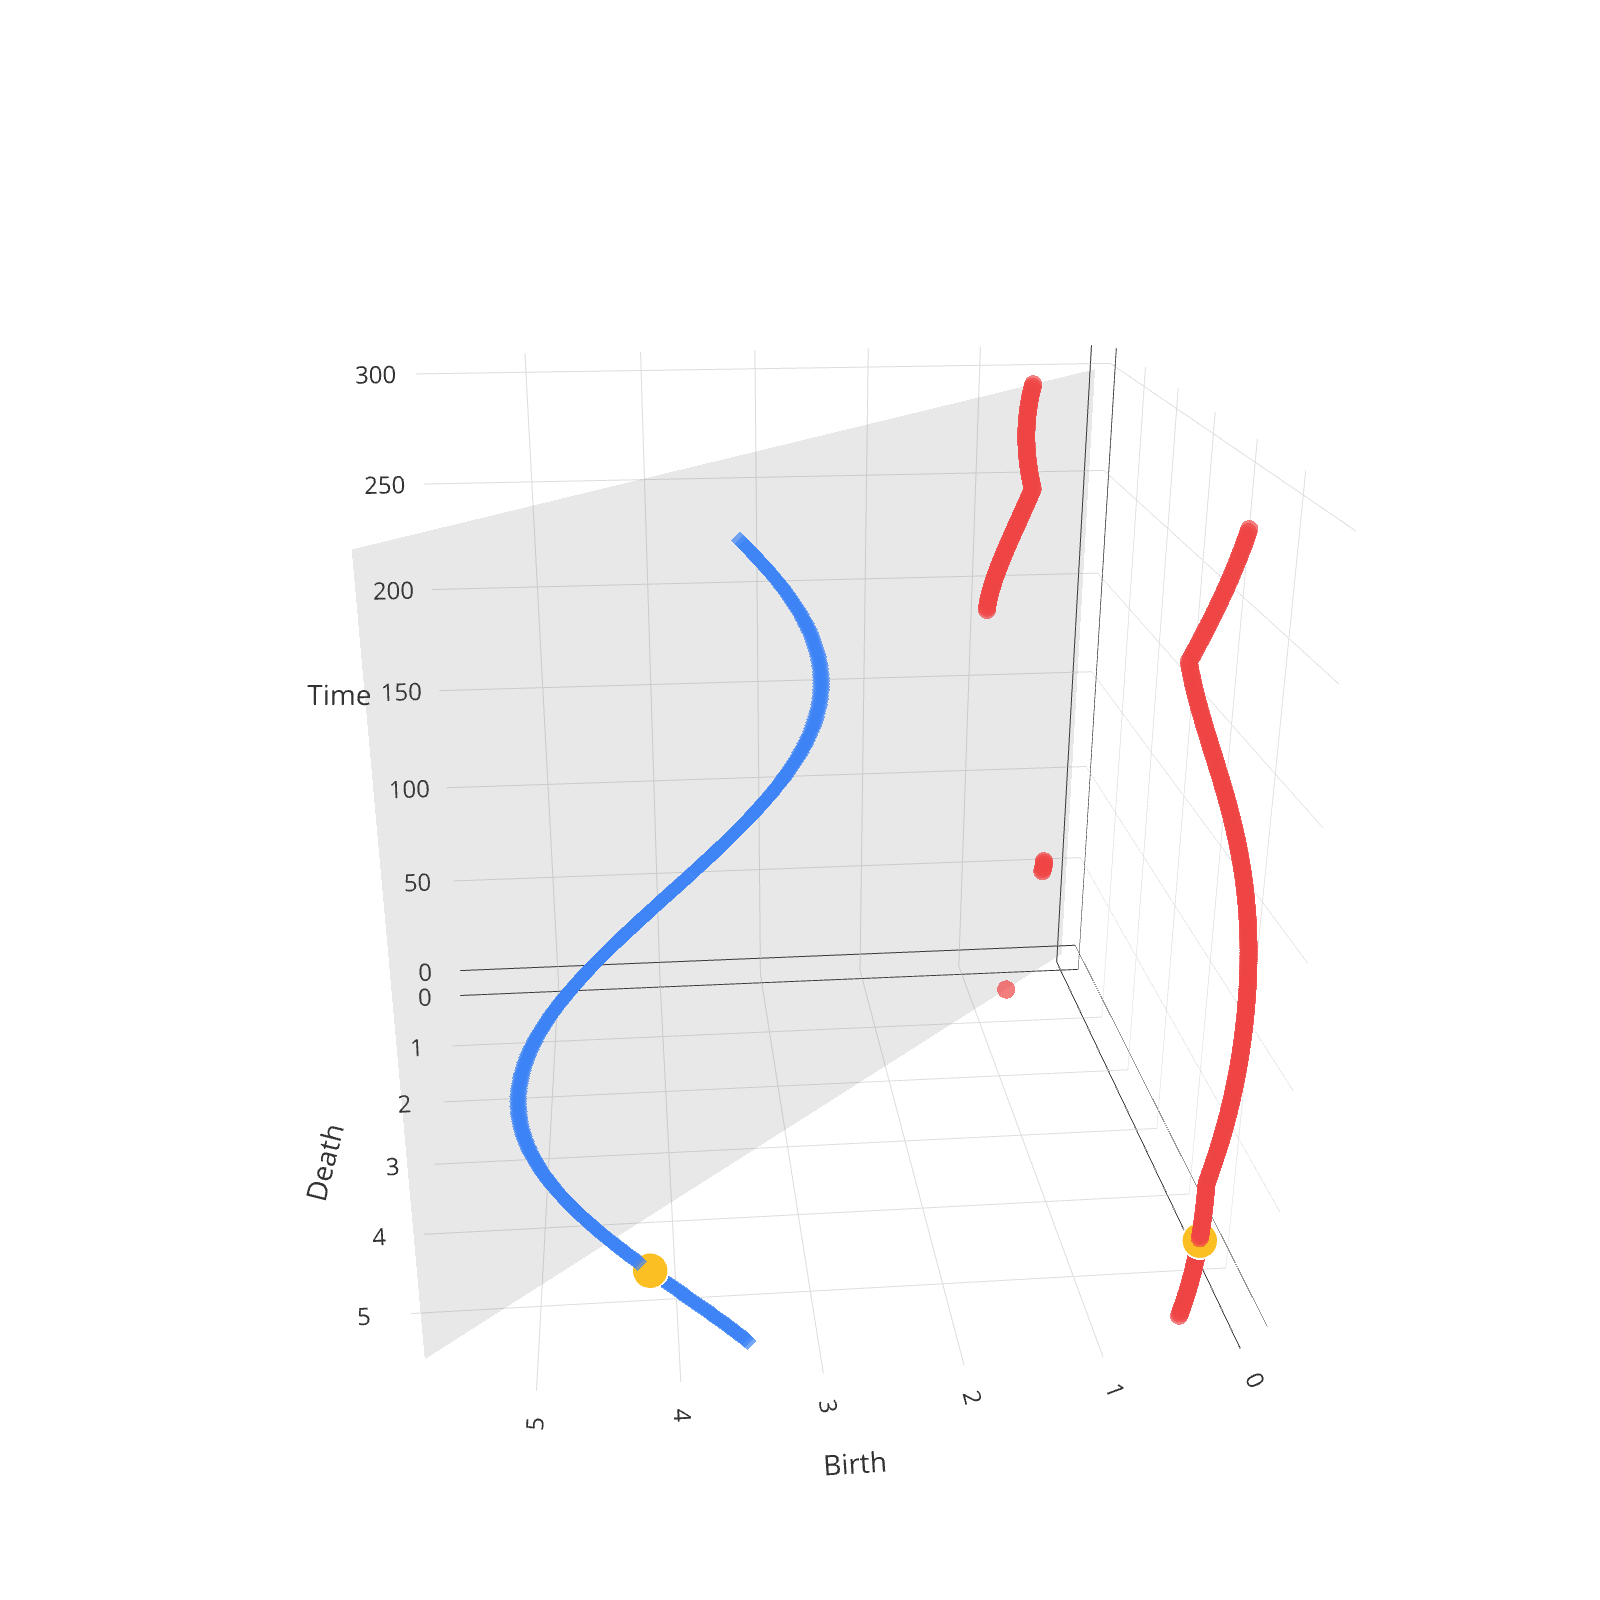
\includegraphics[width=0.47\linewidth]{figures/vin_r1.png}

    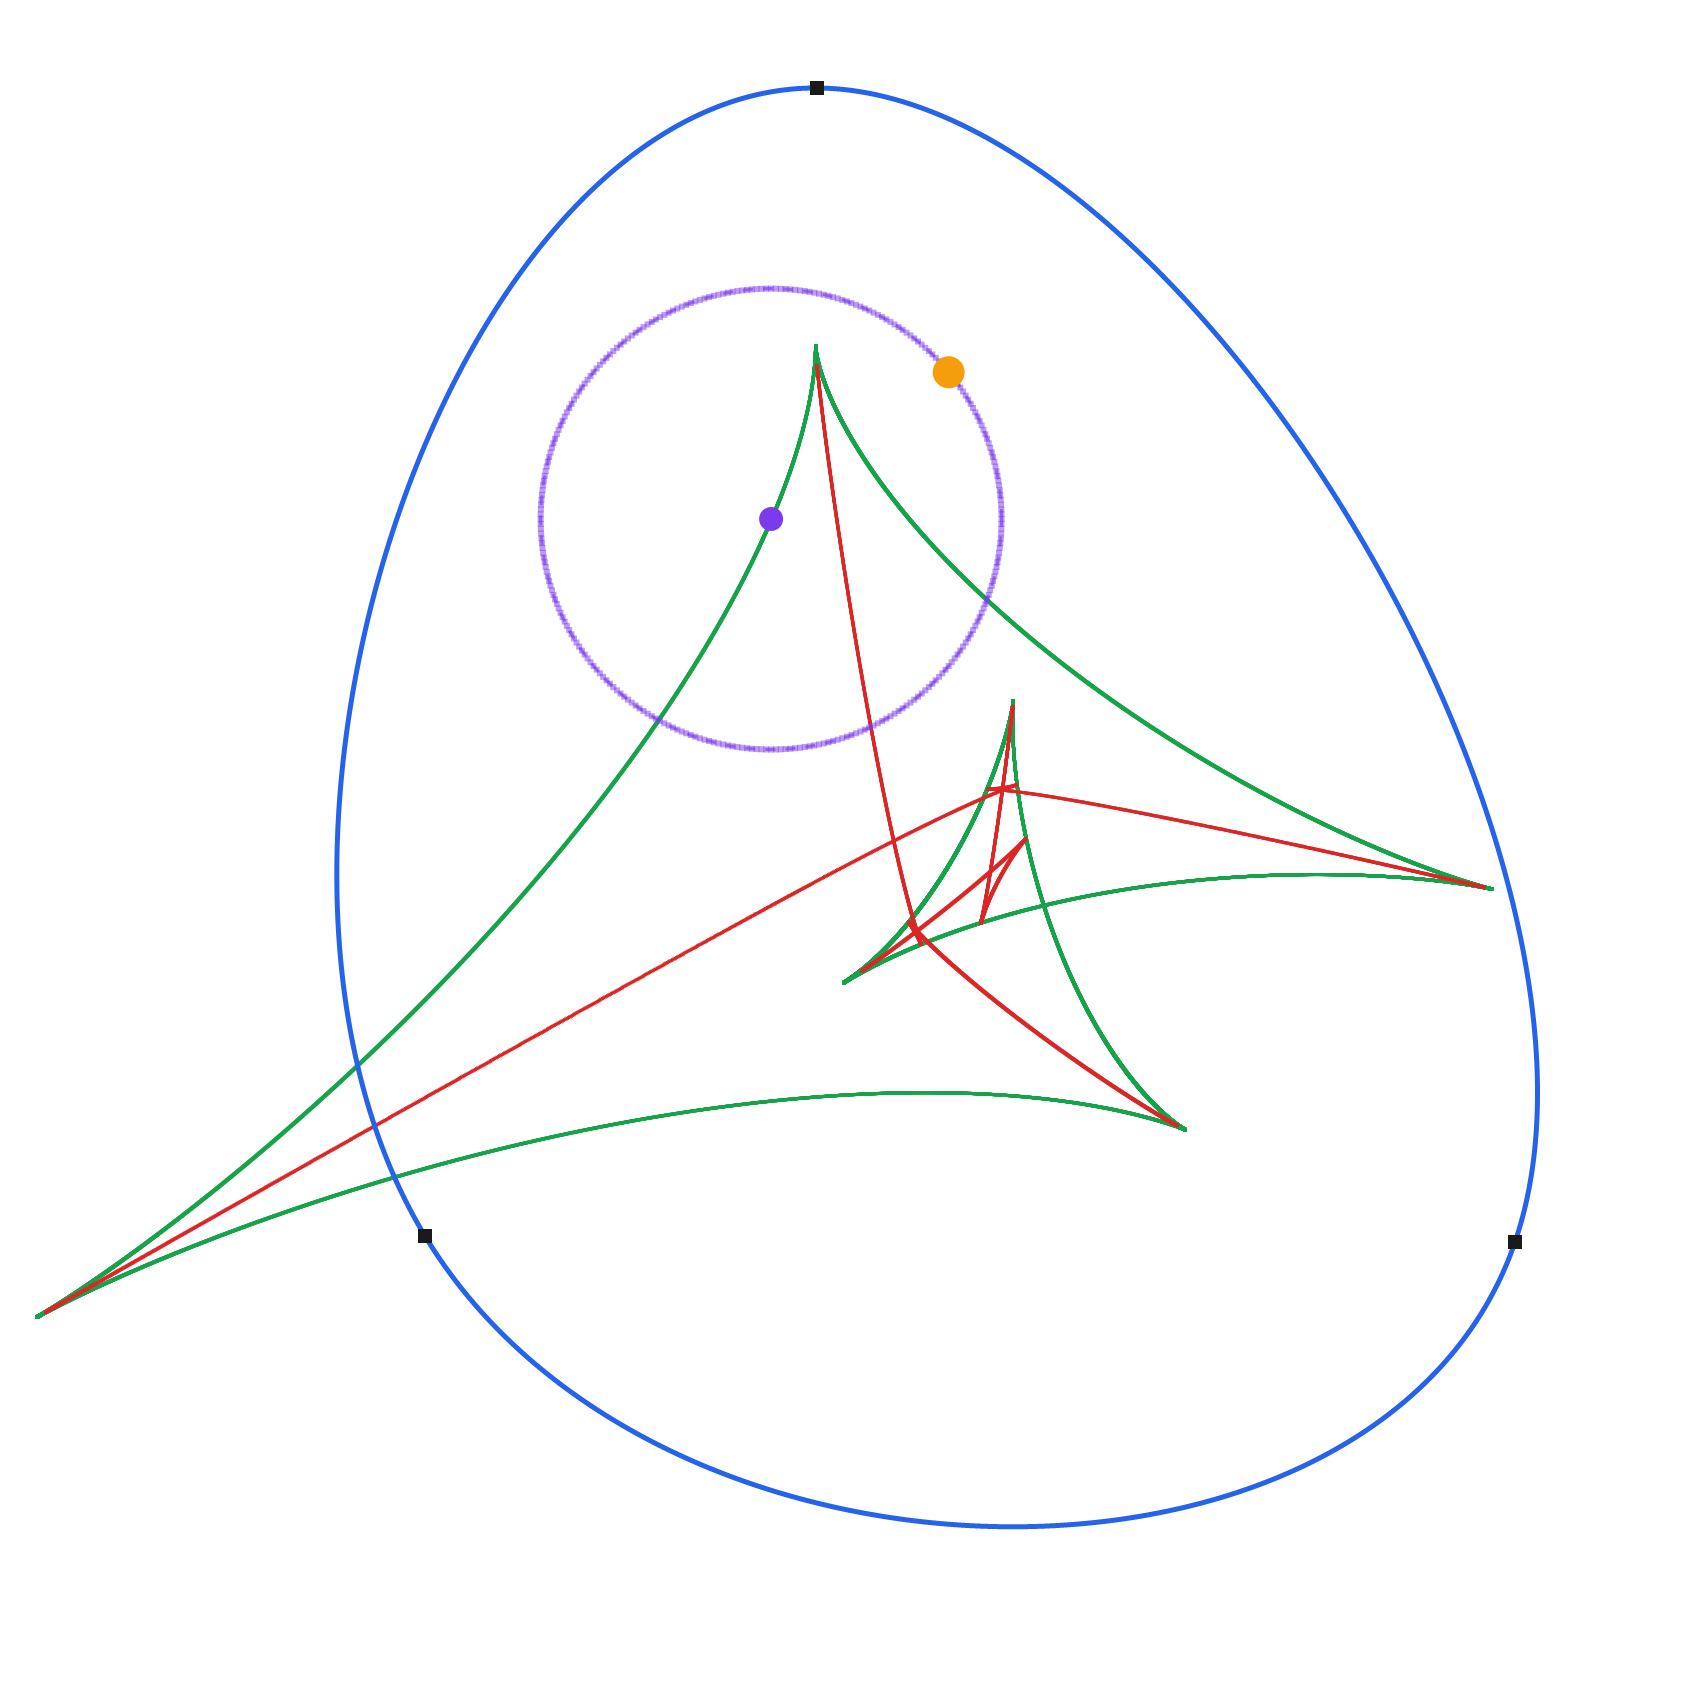
\includegraphics[width=0.47\linewidth]{figures/canvas_r2.png}
    \hfill
    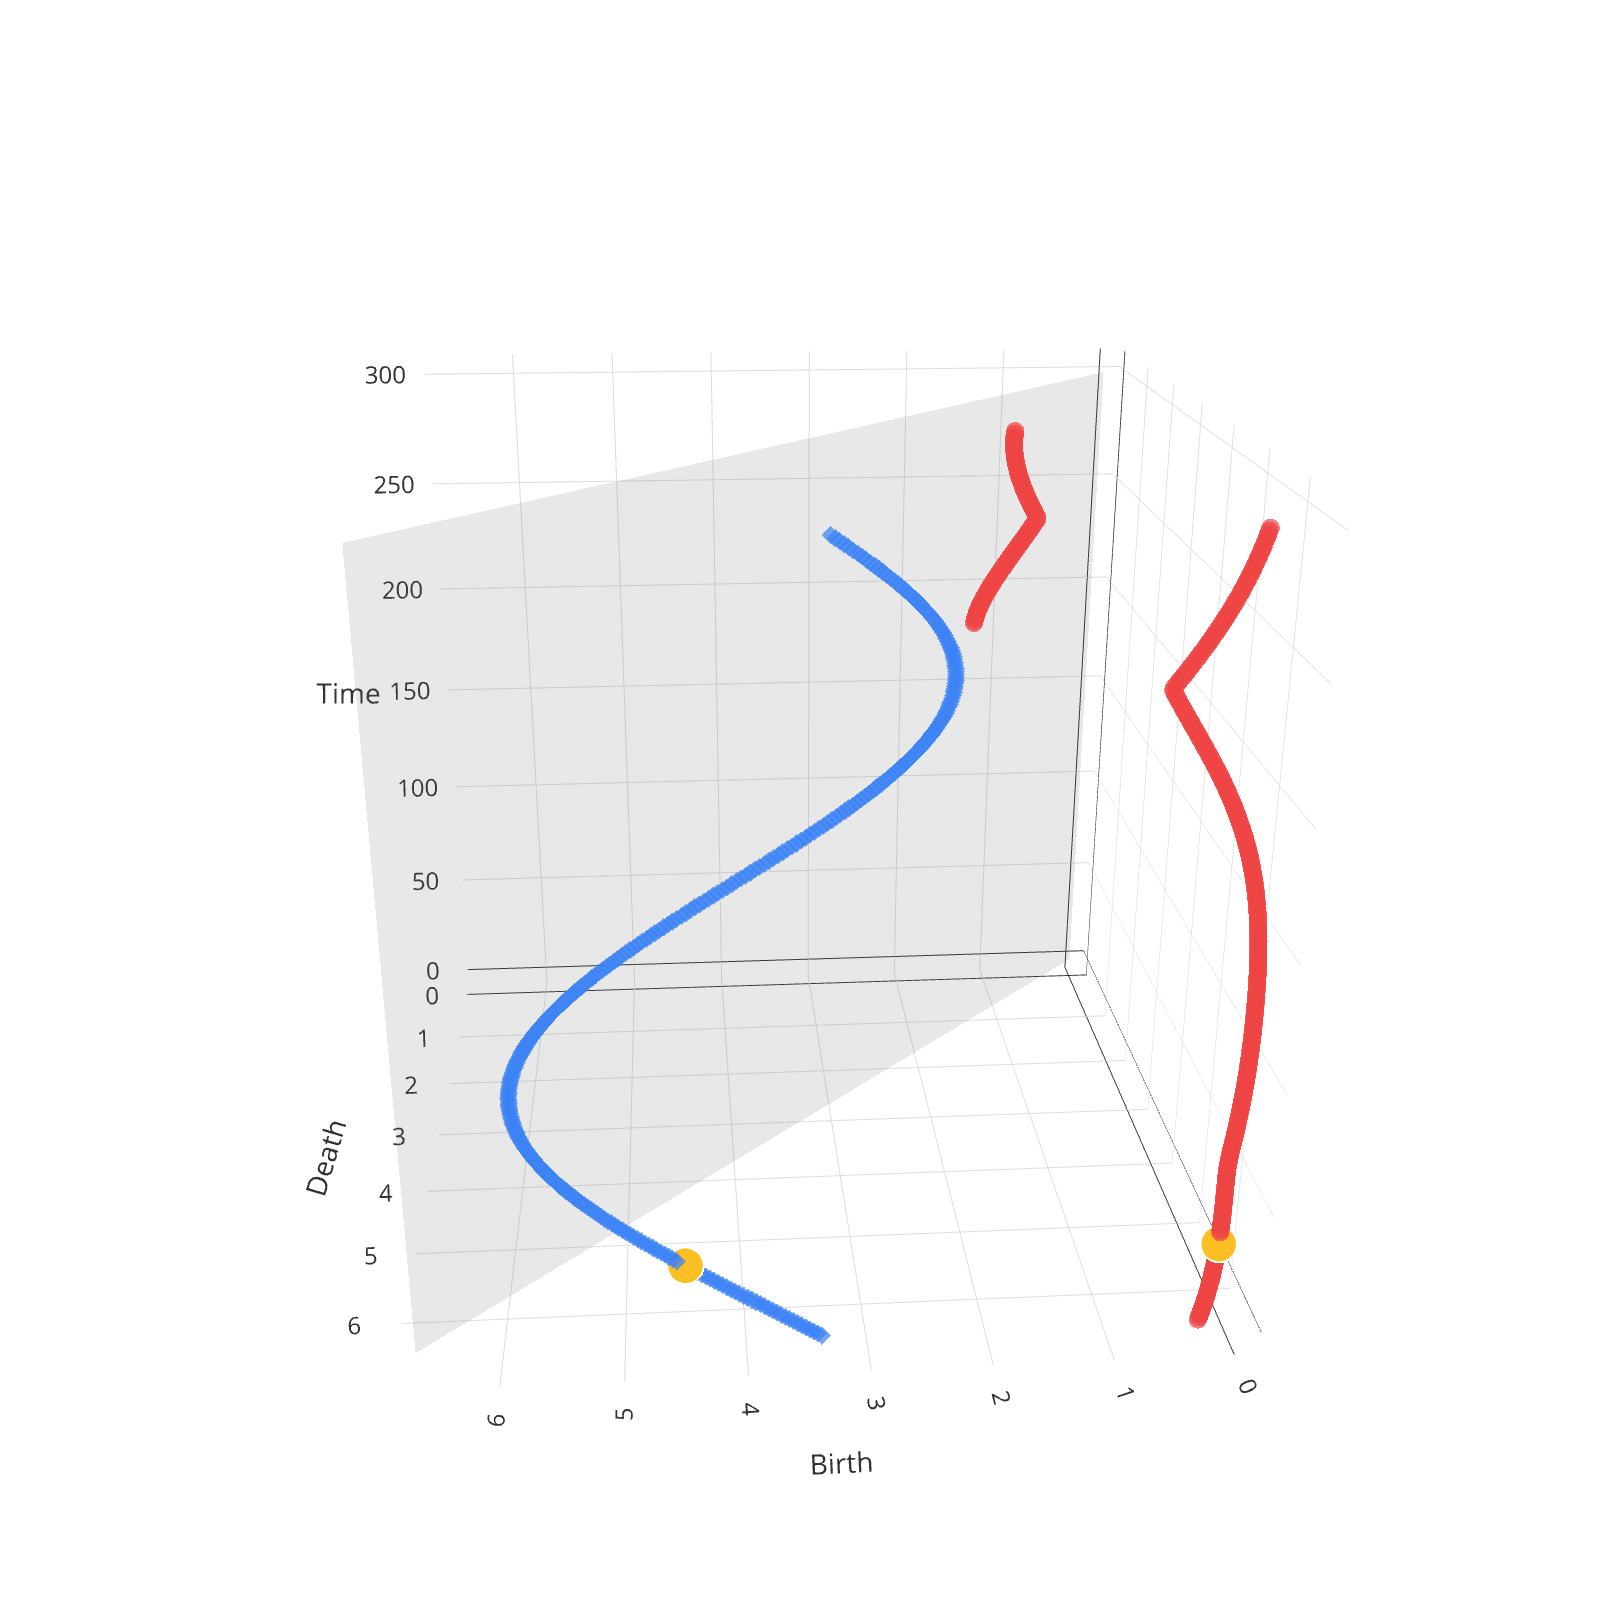
\includegraphics[width=0.47\linewidth]{figures/vin_r2.png}

    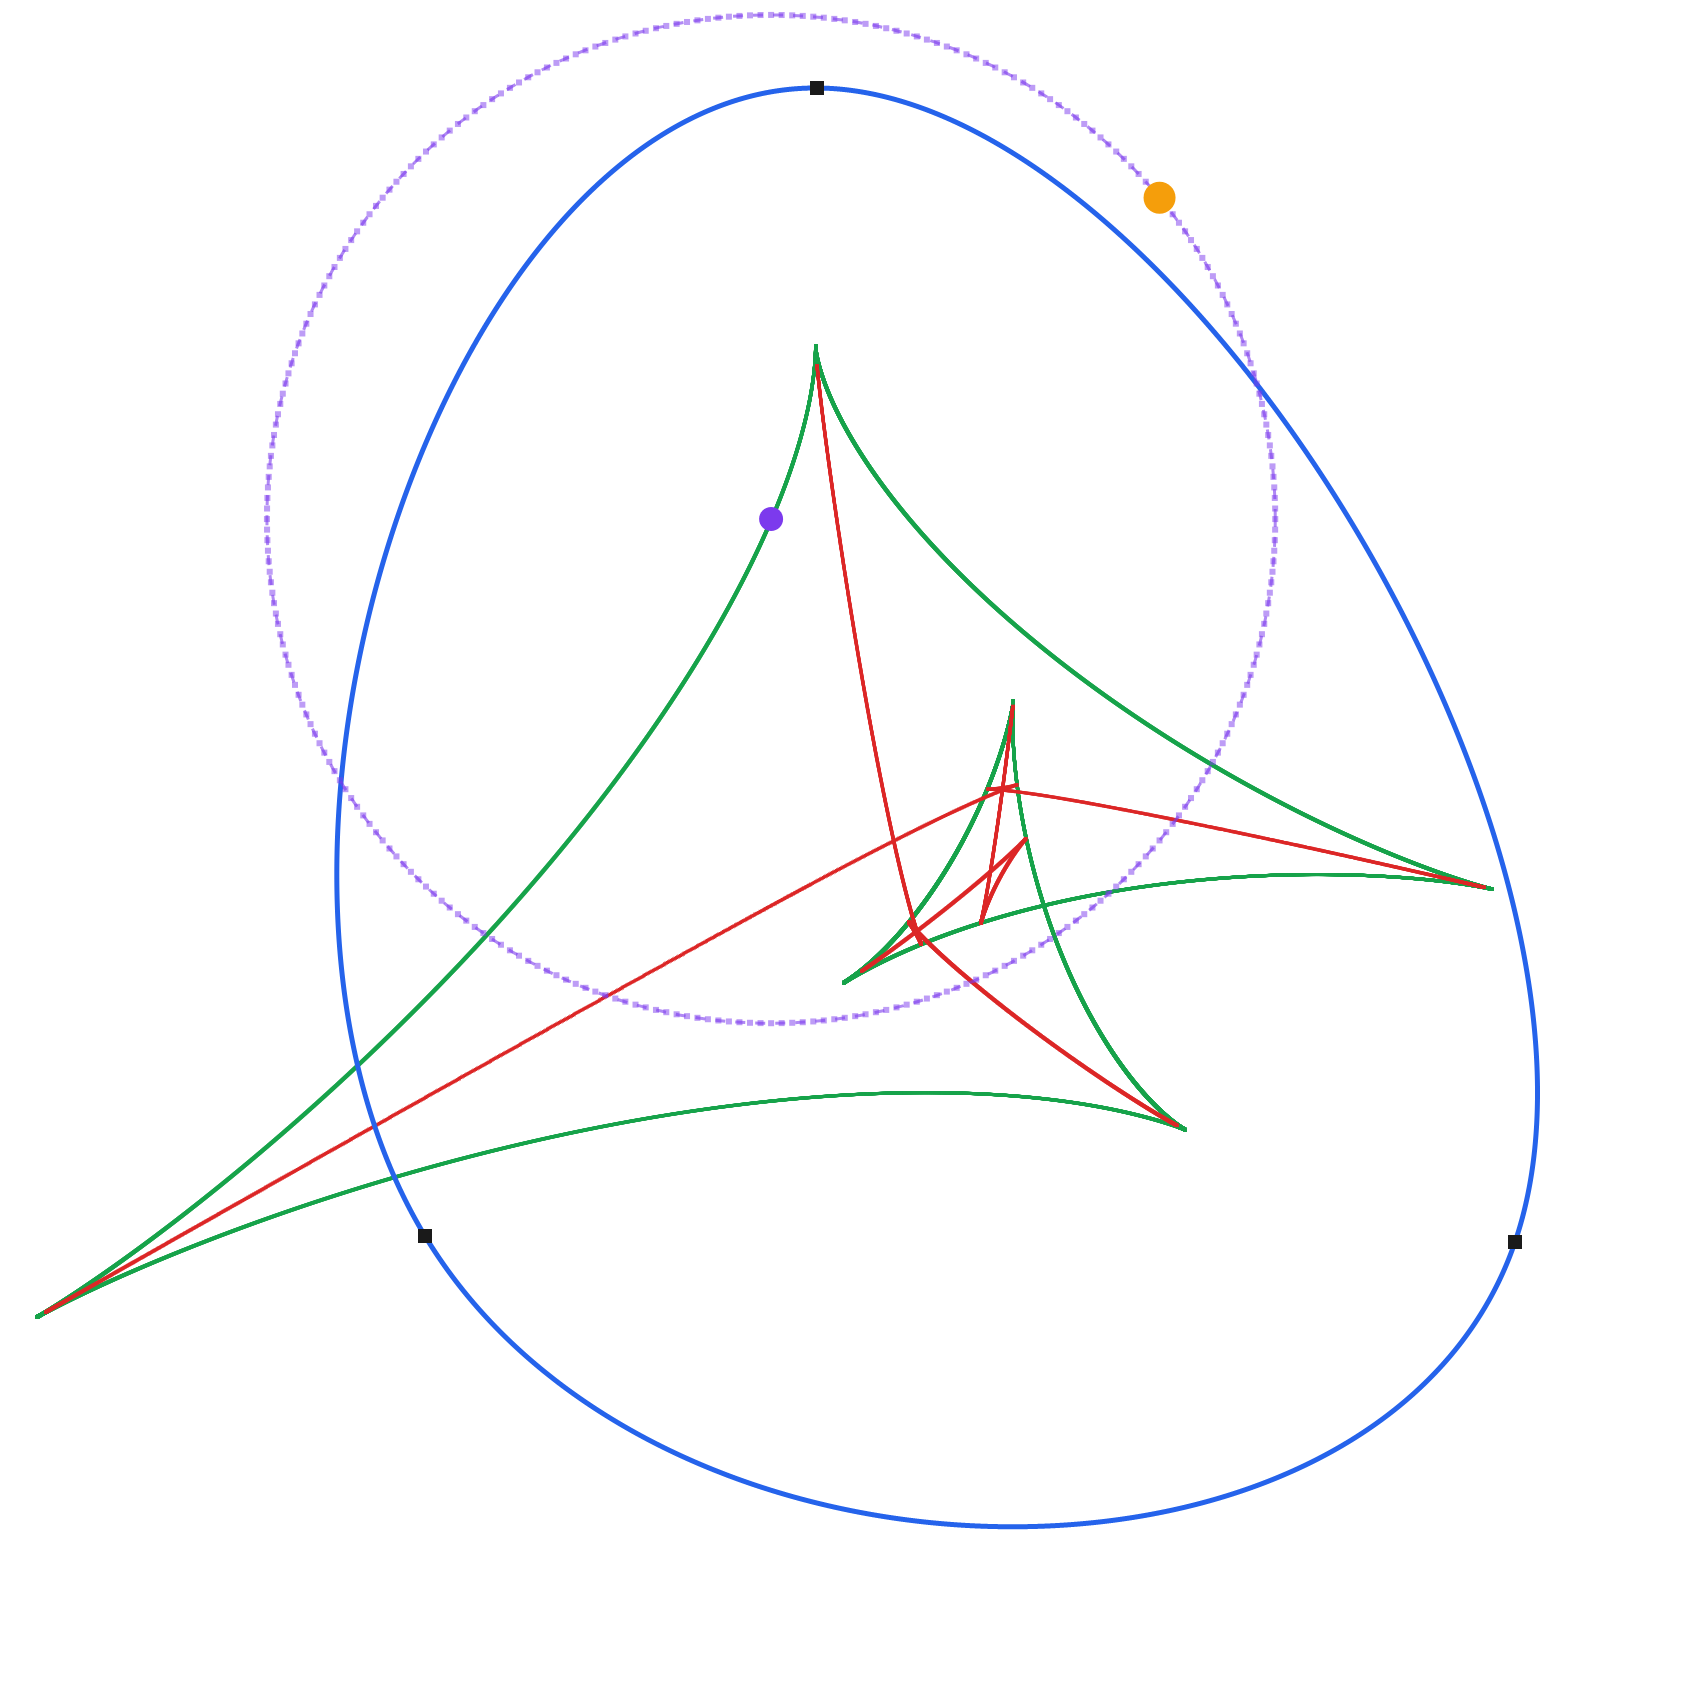
\includegraphics[width=0.47\linewidth]{figures/canvas_r3.png}
    \hfill
    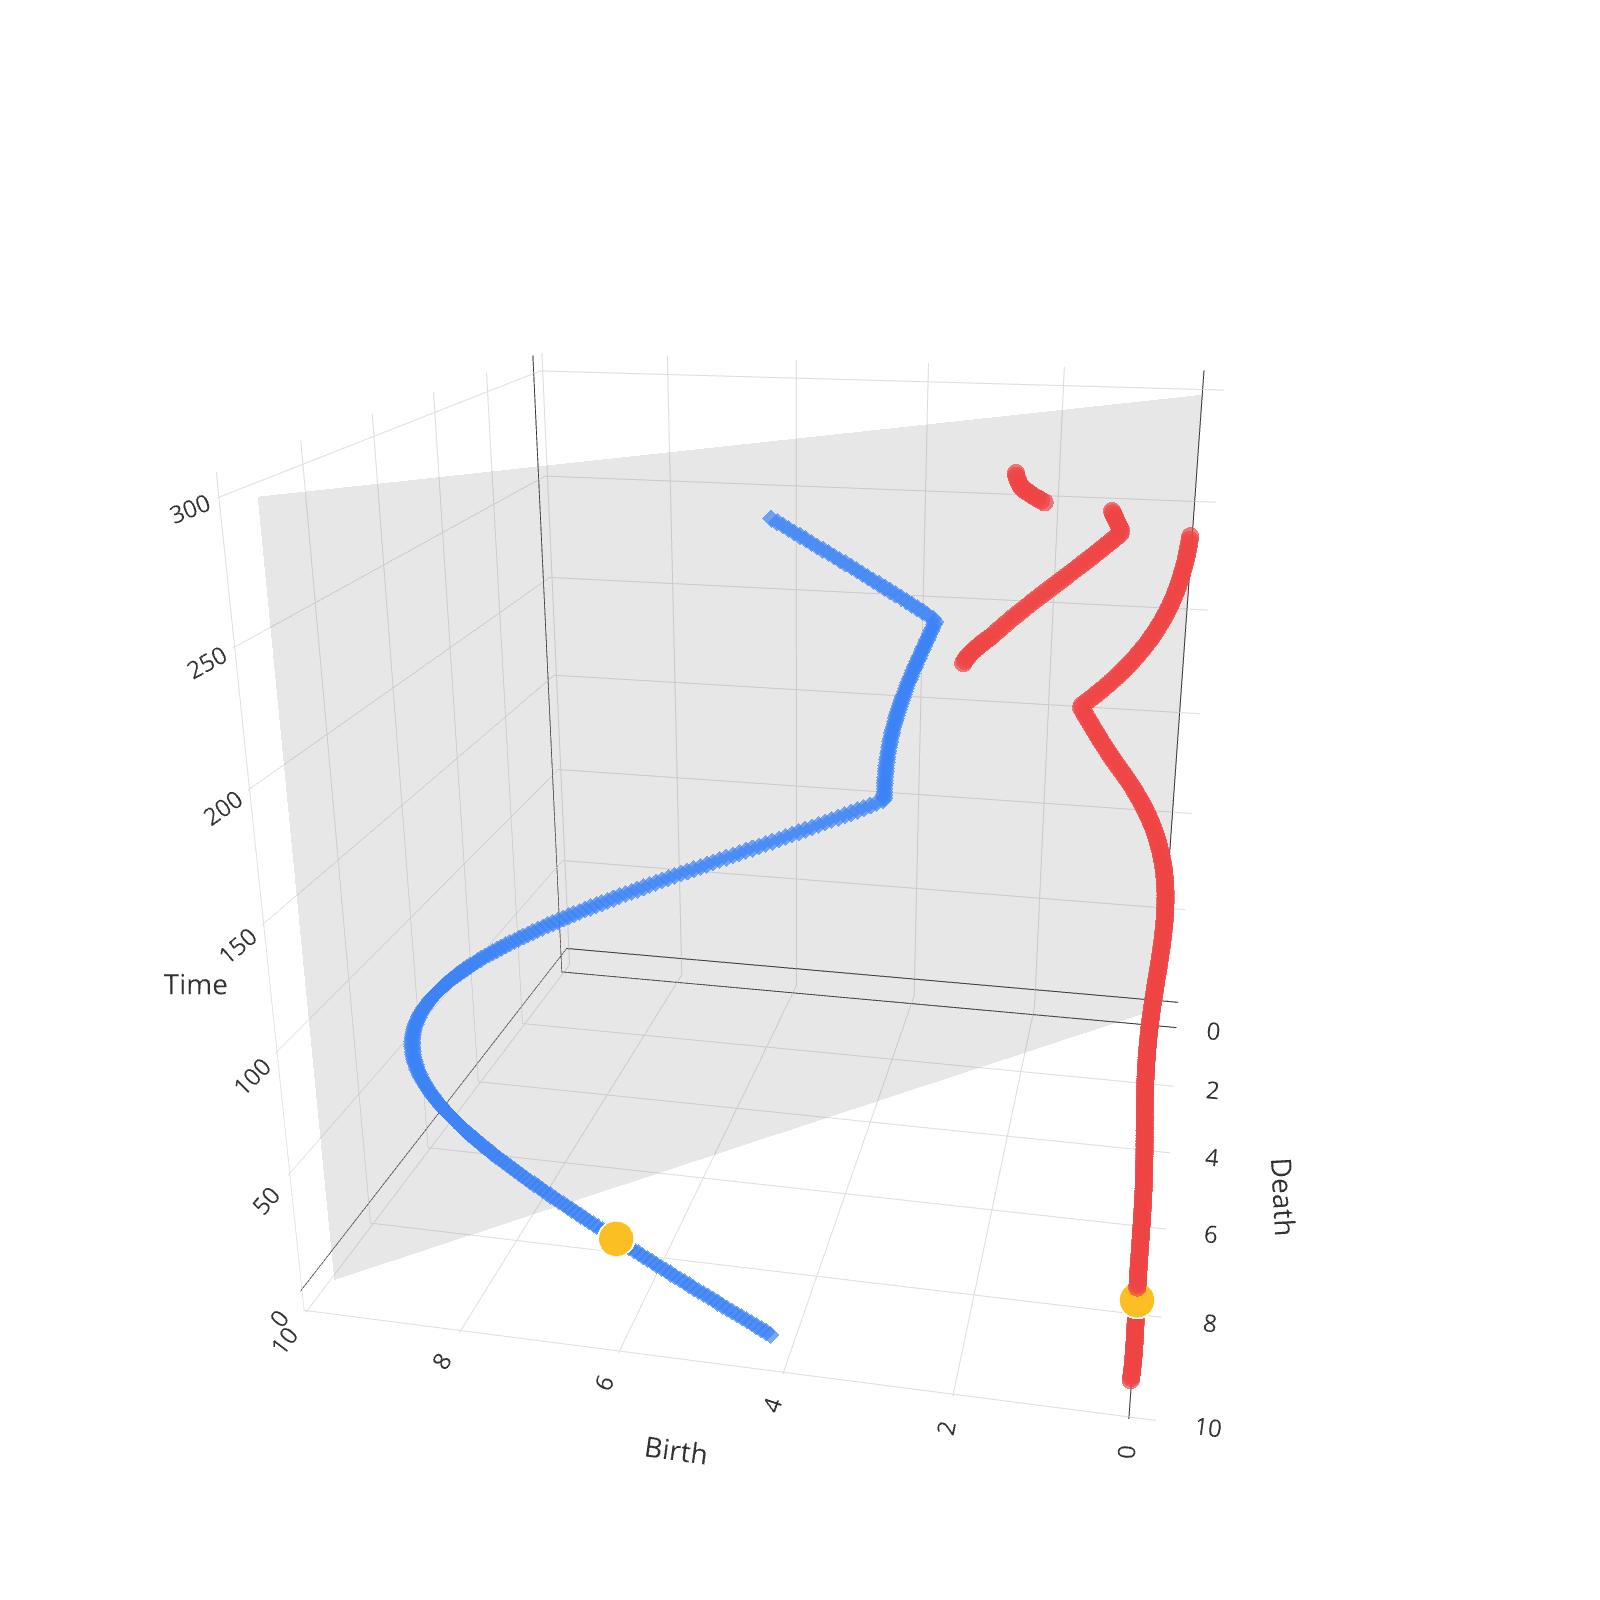
\includegraphics[width=0.47\linewidth]{figures/vin_r3.png}
    \caption{Demonstration about how the vineyard changes as the radius of the center circle changes.}
    \label{fig:vin_change}
\end{figure}

Figure \ref{fig:2_comp} shows a particularly compelling case, where the tool computes the vineyard for two disjoint connected components using extended persistence. This is particularly useful to track global spatial relationships along the observation loop.

\begin{figure}
    \centering
    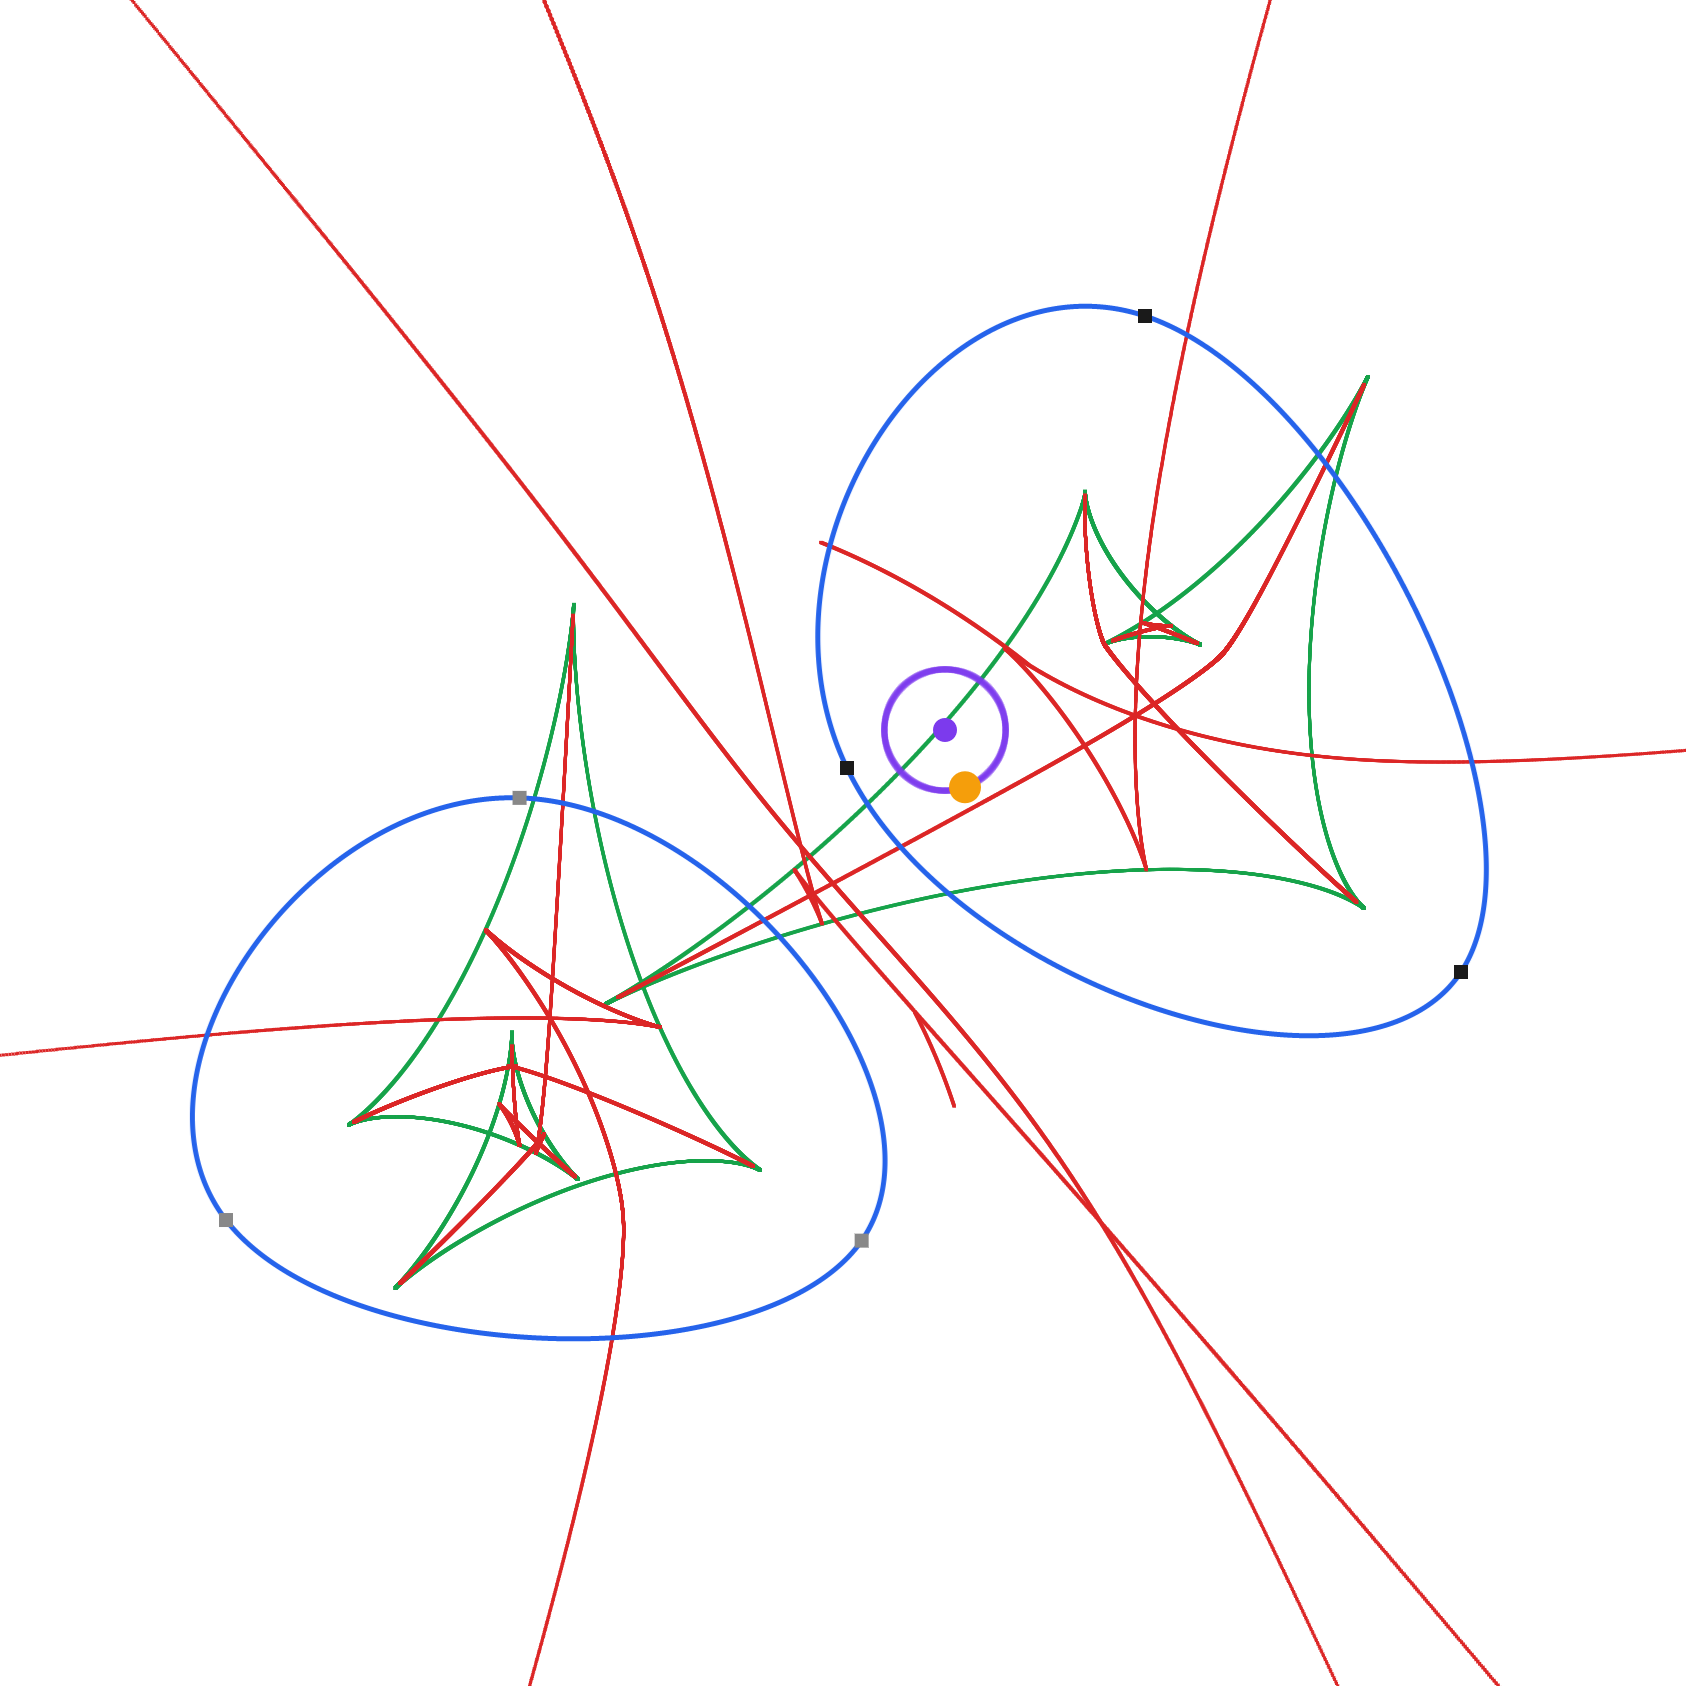
\includegraphics[width=0.47\linewidth]{figures/2_comp_vin.png}
    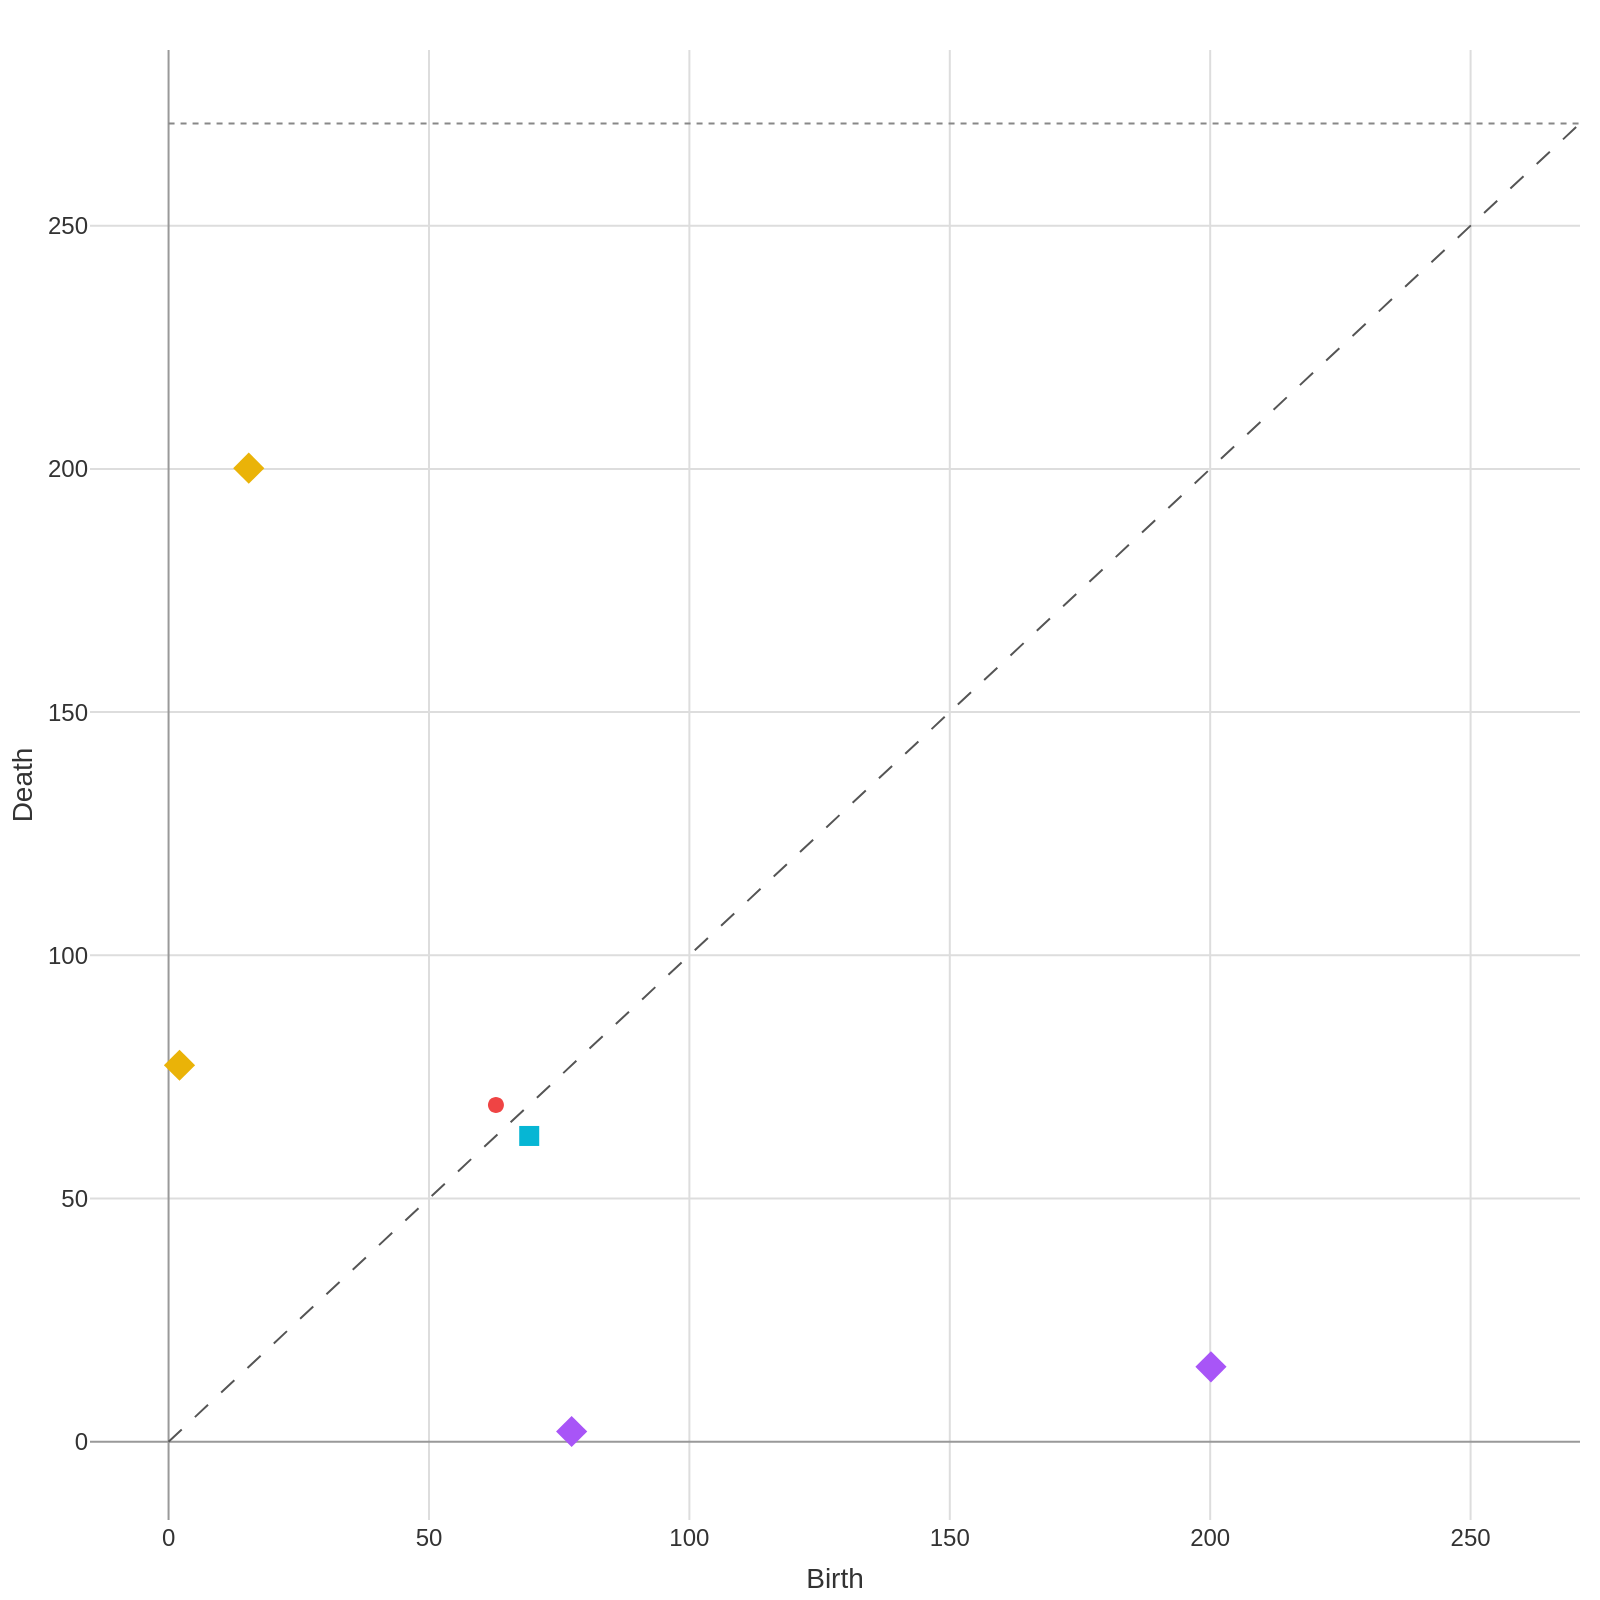
\includegraphics[width=0.47\linewidth]{figures/pd_2_comp.png}
    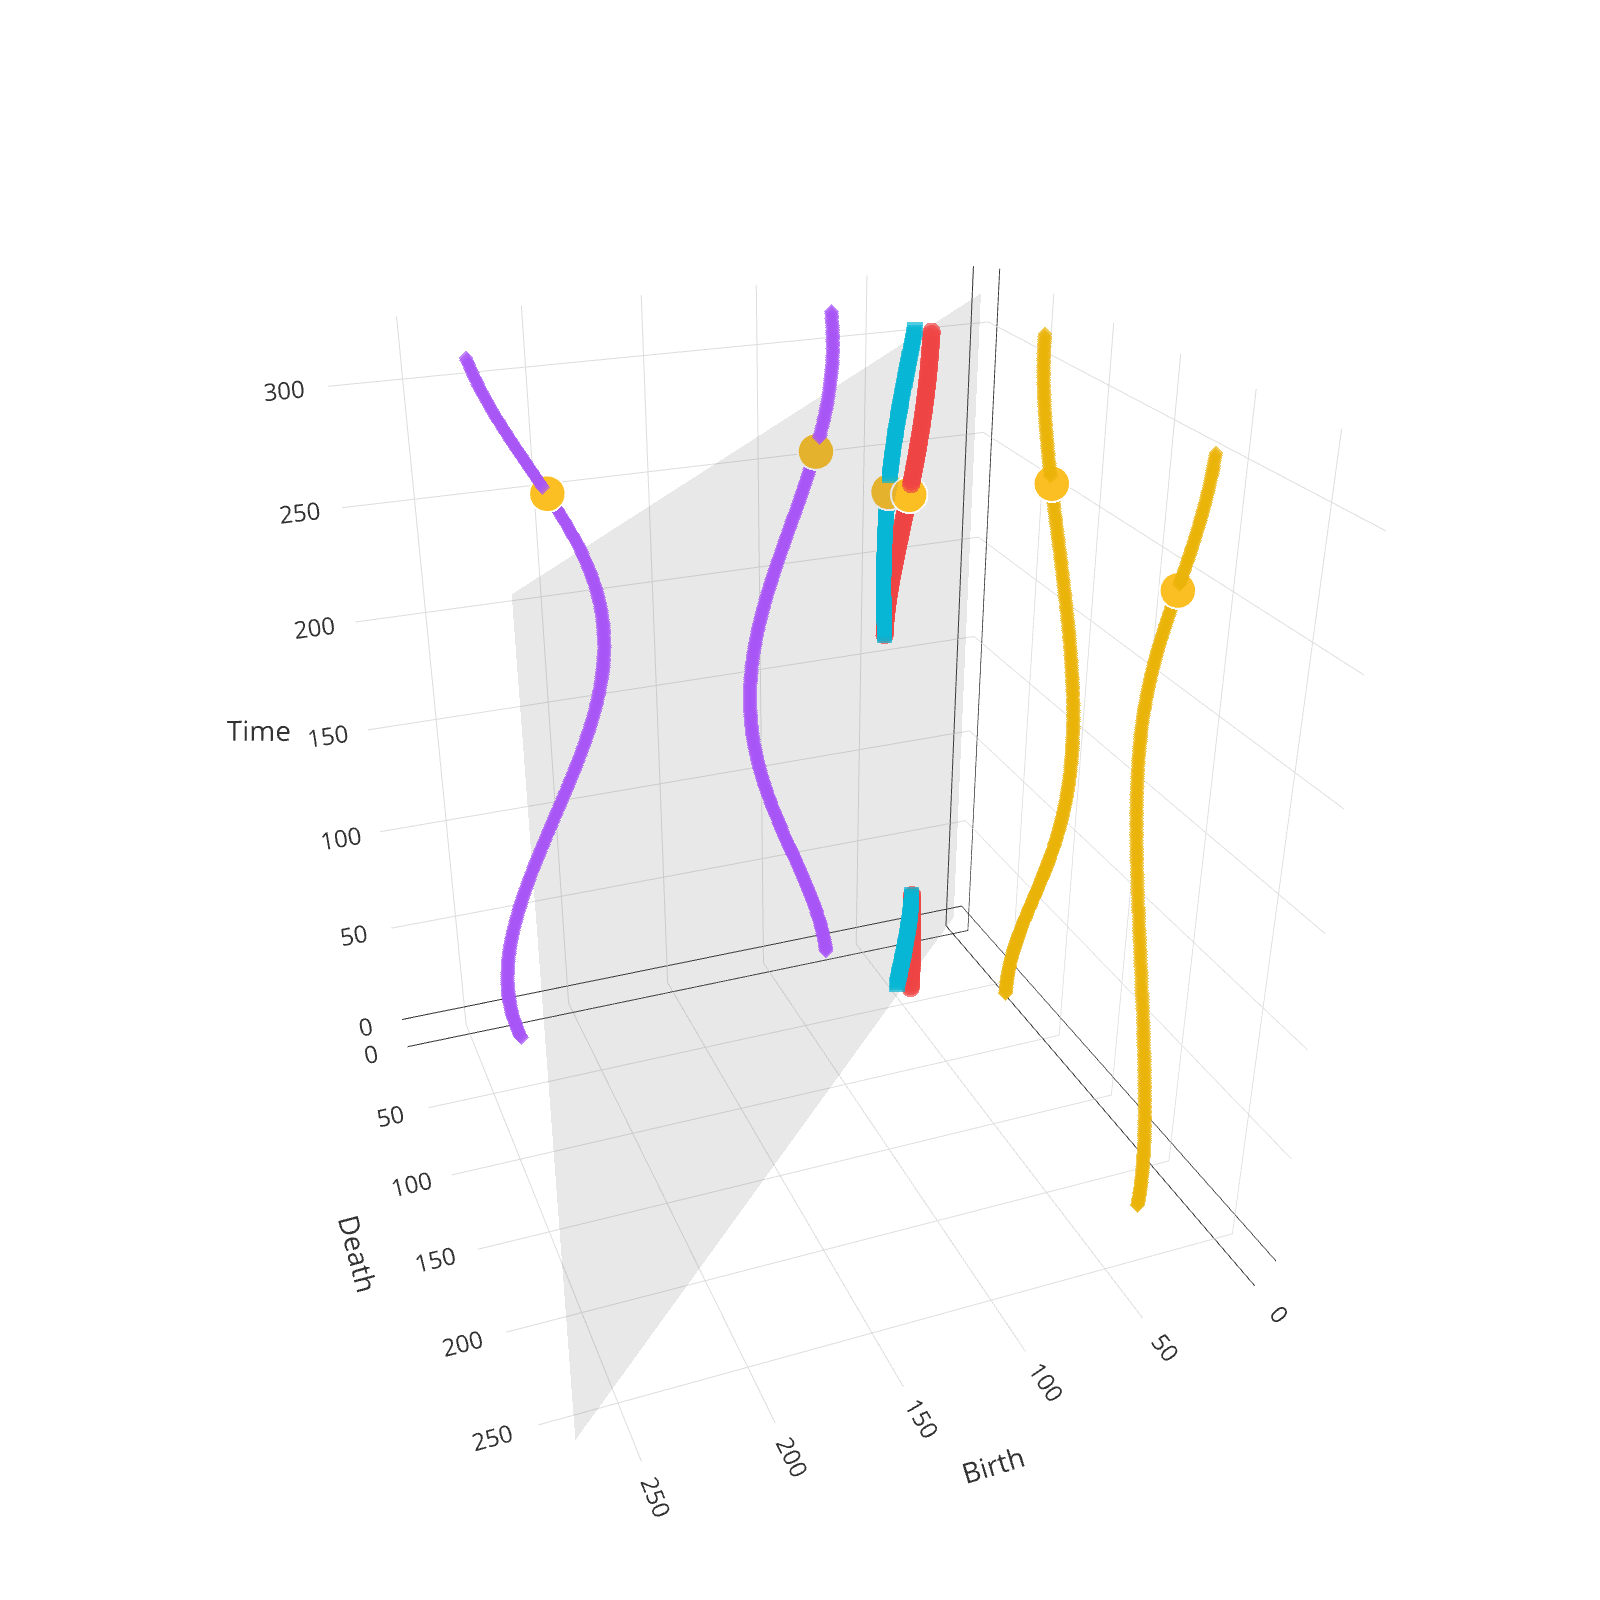
\includegraphics[width=0.6\linewidth]{figures/vin_2_comp.png}
    \caption{Demonstration of a vineyard for 2 disjoint connected components, with extended persistence.}
    \label{fig:2_comp}
\end{figure}

Figure \ref{fig:spline_obs} is a demonstration of a vineyard where the measurement center moves along a arbitrary hand-drawn loop via splines; the resulting vineyard captures the topological response to a non-standard path, illustrating how custom trajectories can be used to probe specific regions of the ambient space.

\begin{figure}
    \centering
    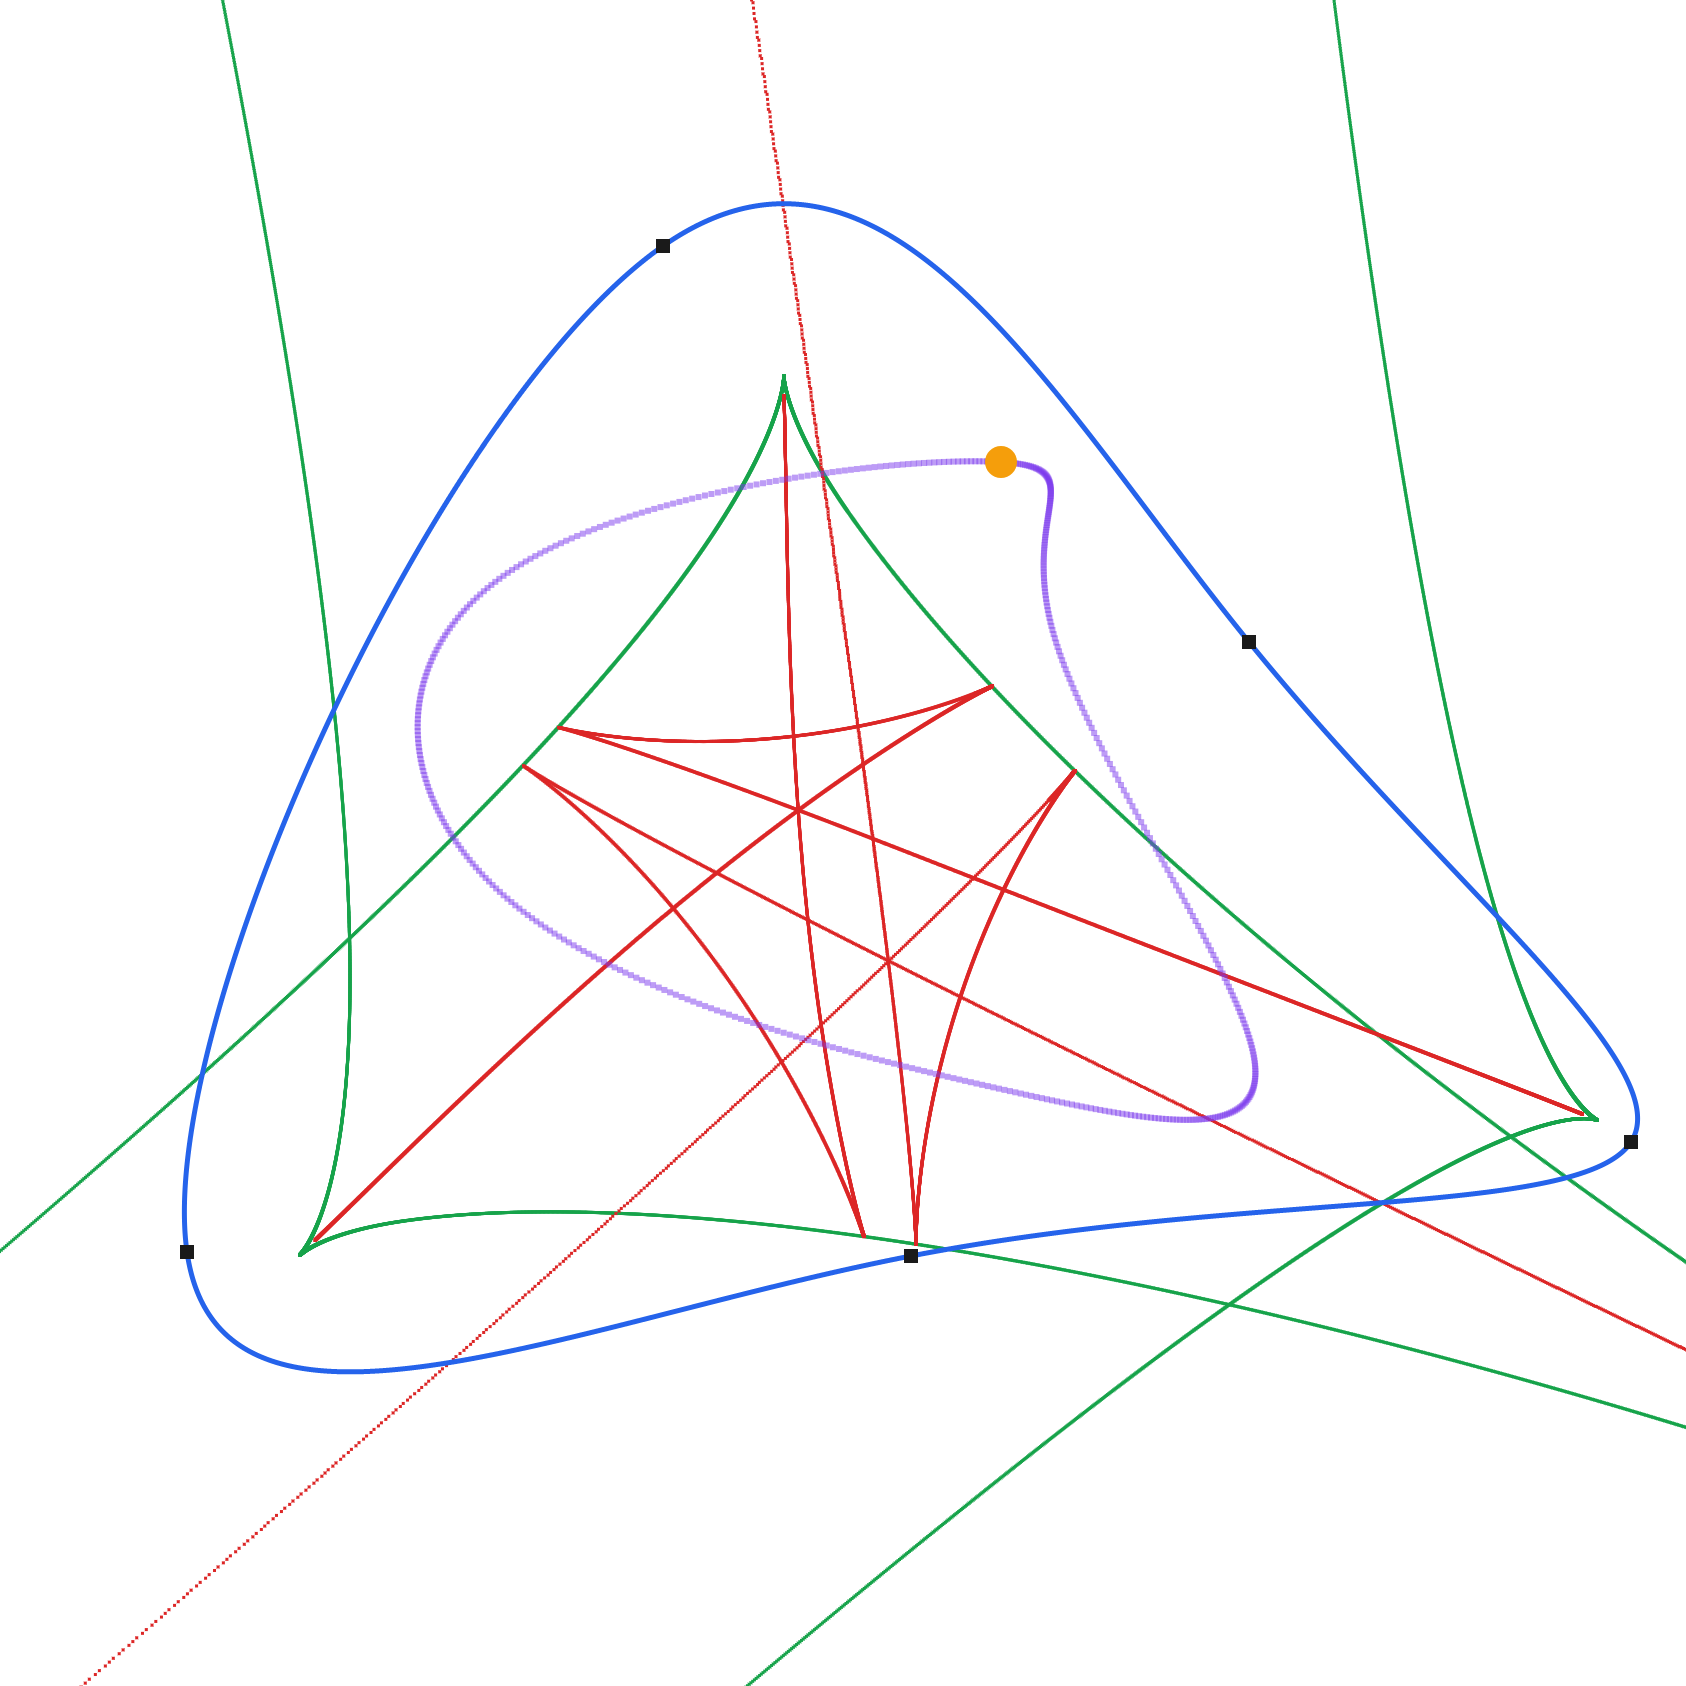
\includegraphics[width=0.47\linewidth]{figures/canvas_spline.png}
    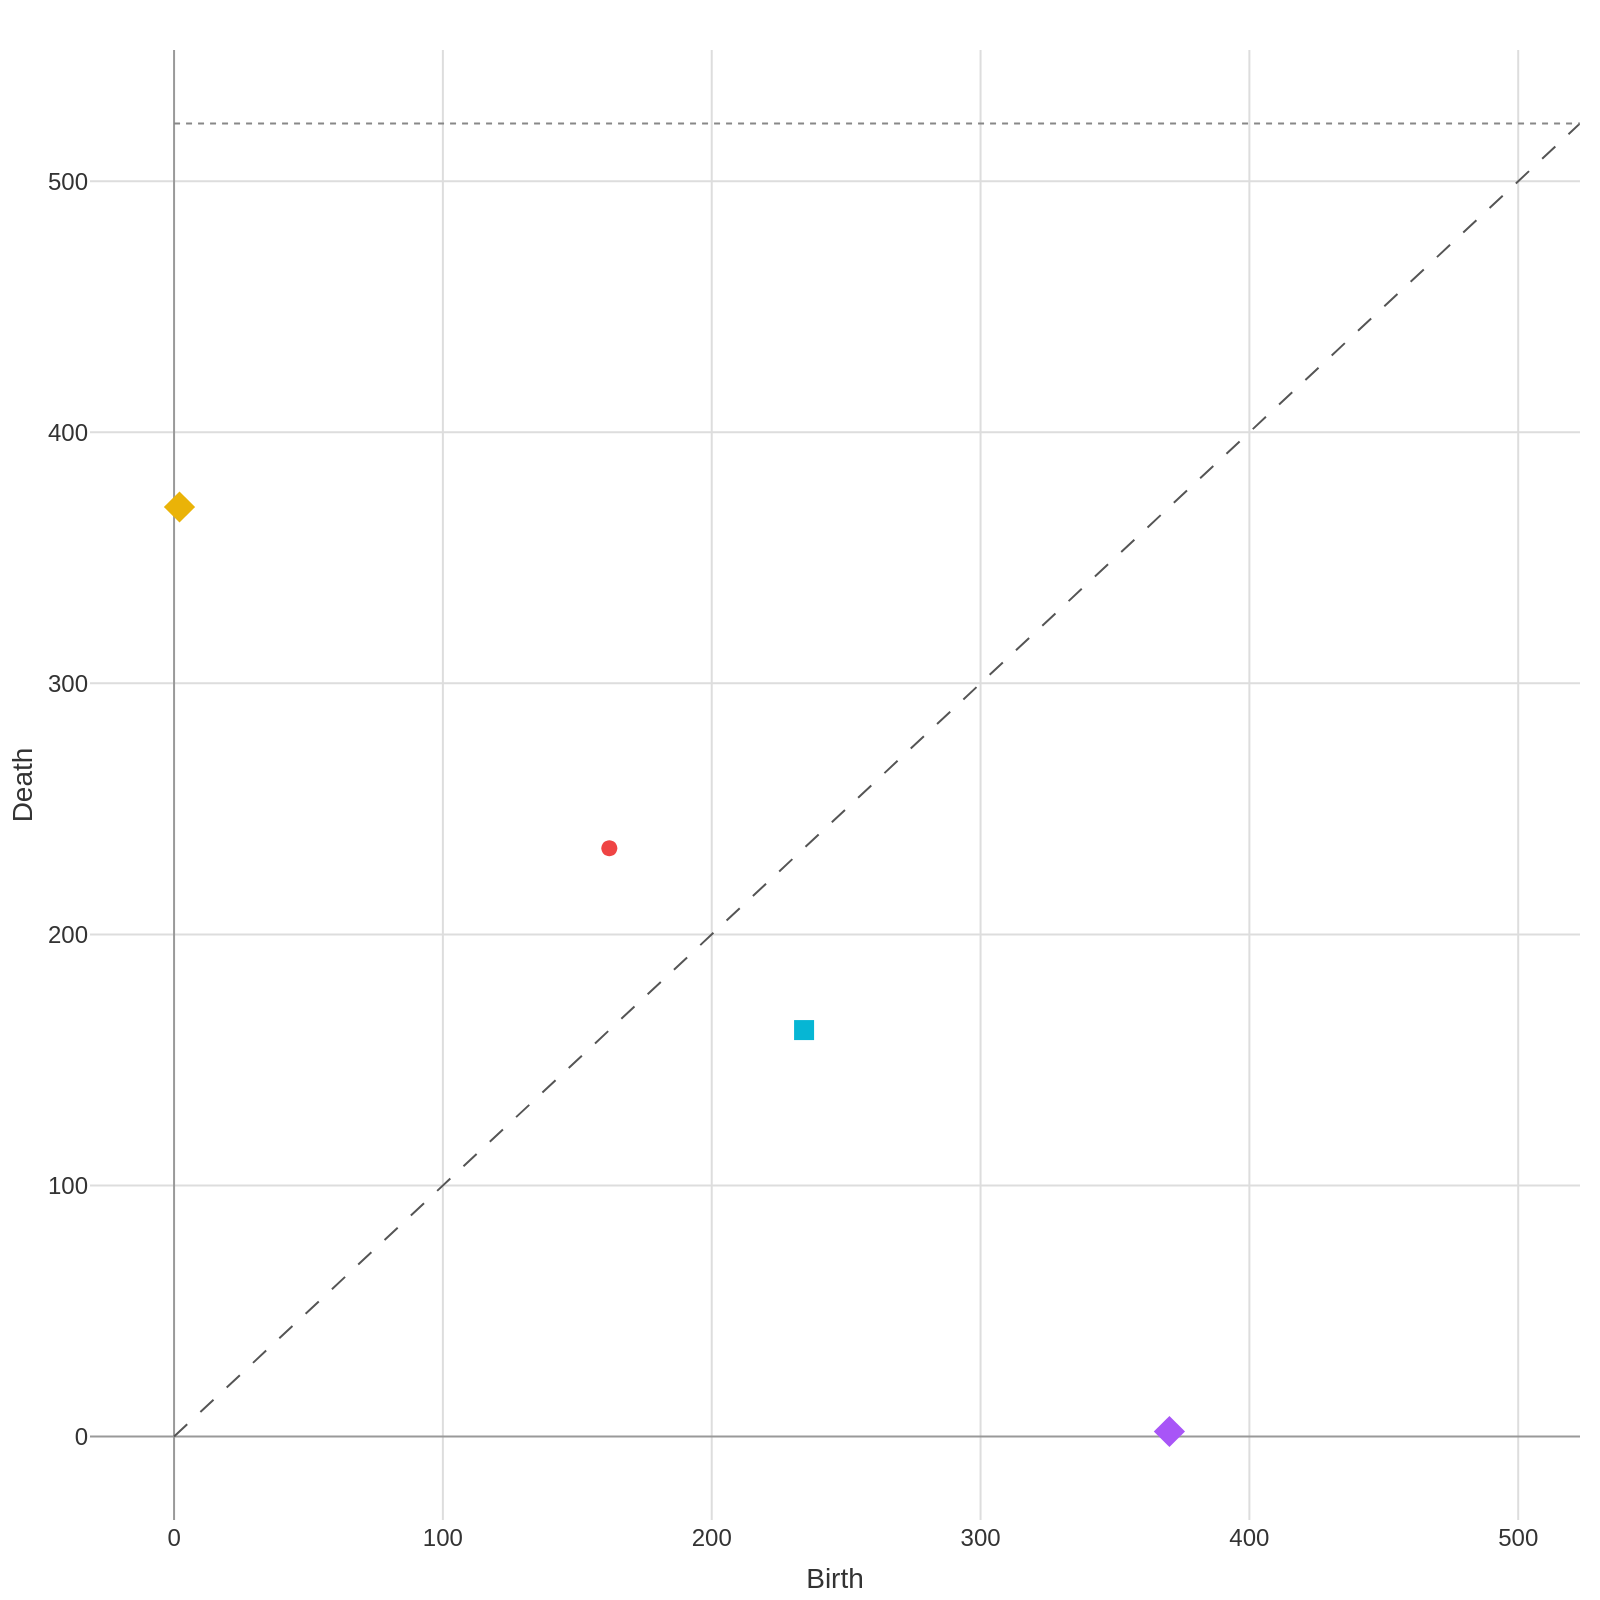
\includegraphics[width=0.47\linewidth]{figures/persistence_diagram_spline.png}
    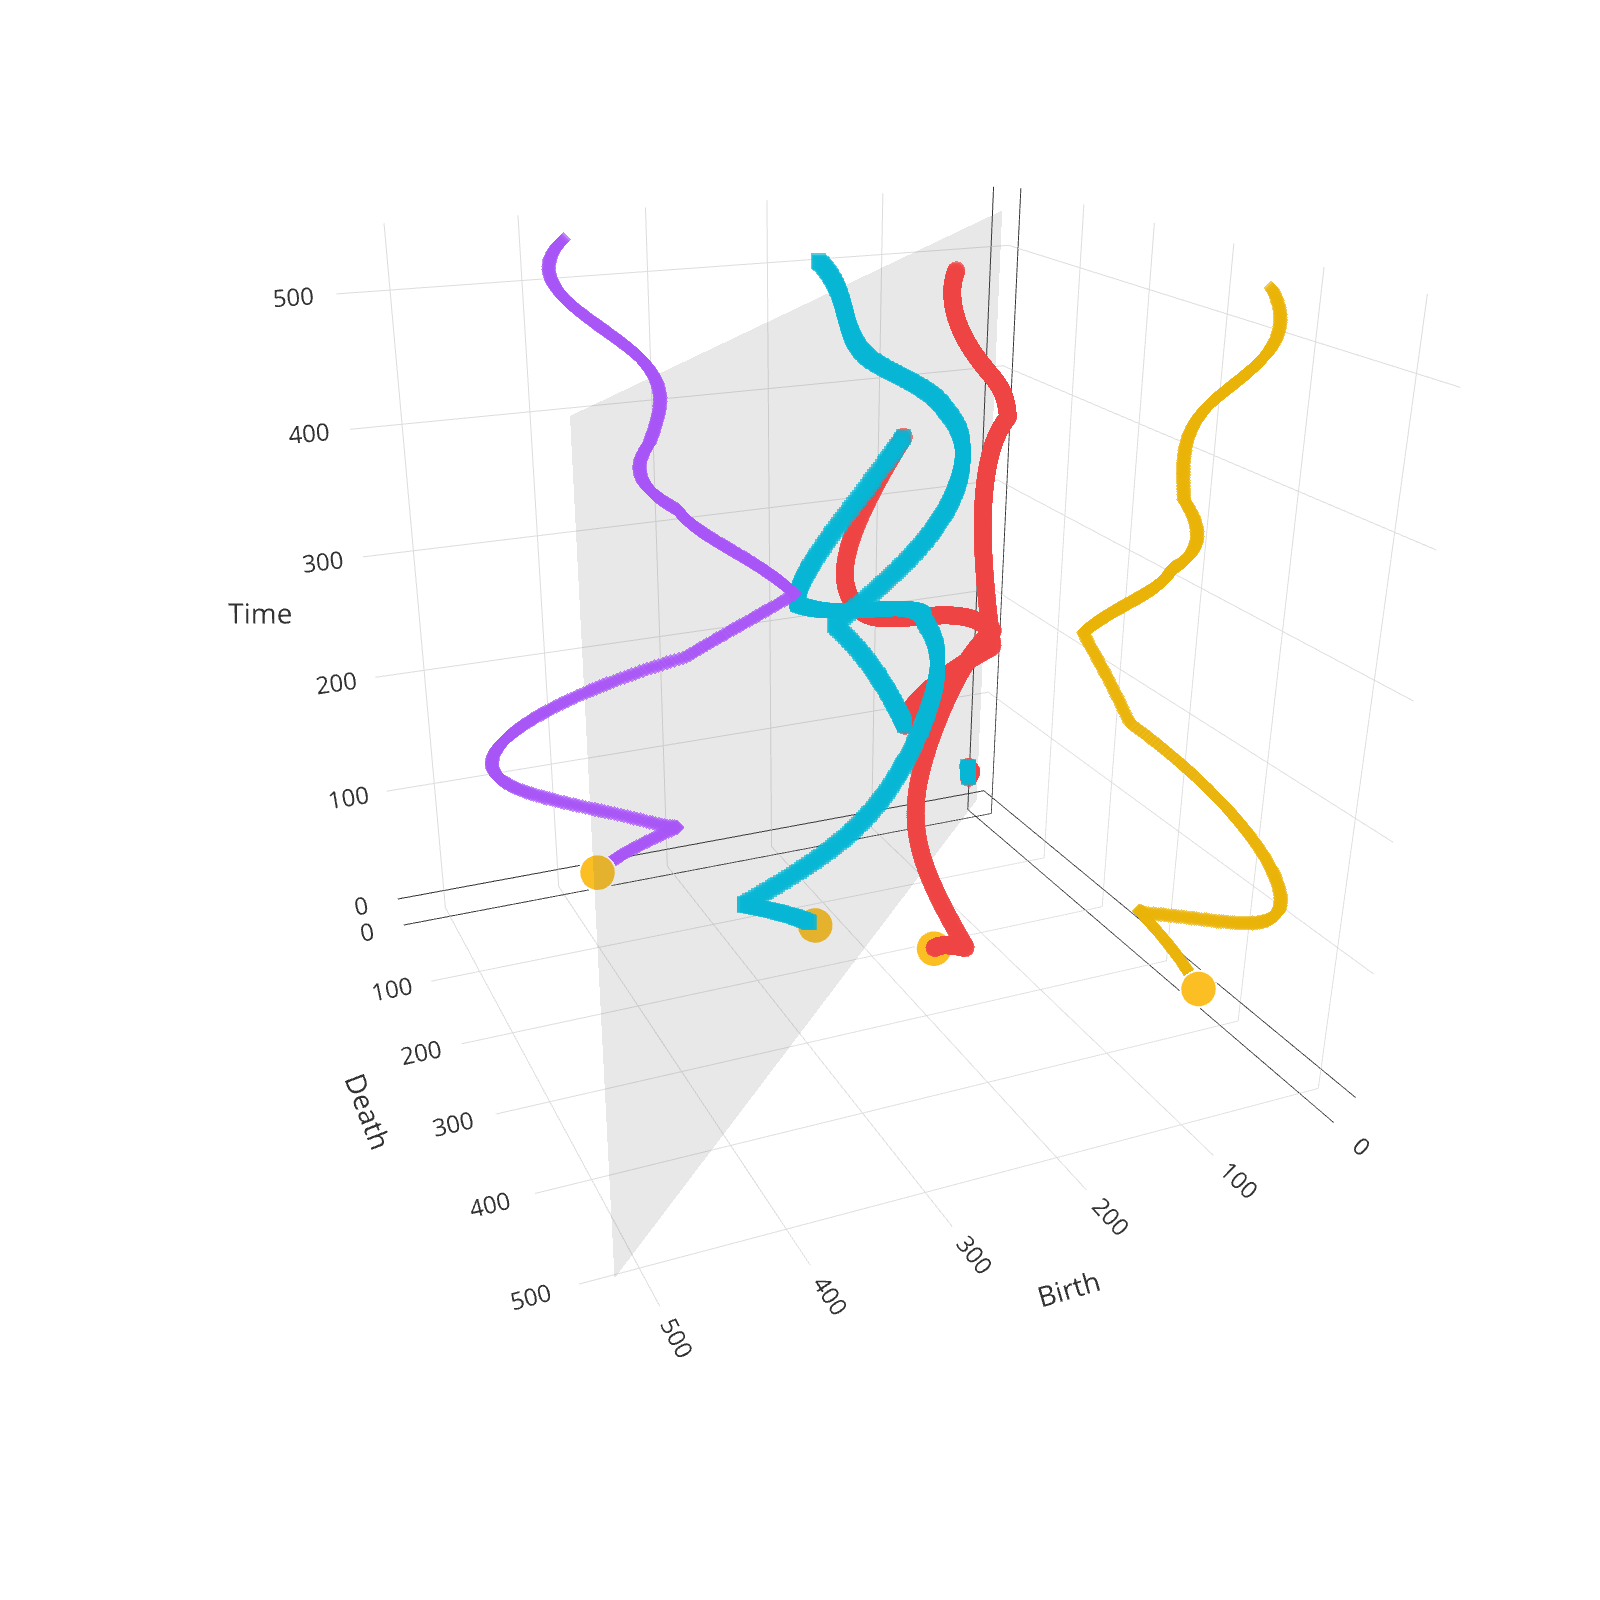
\includegraphics[width=0.6\linewidth]{figures/vin_spline.png}
    \caption{Vineyard for a arbitrary hand-drawn observation loop.}
    \label{fig:spline_obs}
\end{figure}

\section{Outlook: Feedback please!}

We invite everyone %members of the community 
to test the tool and provide feedback and comments on how it can be improved. Currently it supports 2D only. Future works will include extensions to higher dimensions.

% \subsection{Problem Statement and Solution}

% \subsubsection{Problem Setup}

% We consider only the two-dimensional setting.
% We assume \dots

% \subparagraph{Precise Problem Formulation.}

% Describe your problem as clearly as possibly, instead of the usual \dots

% \begin{conj}
% Could it really be like this?
% \end{conj}
% \begin{obs}
% Probably not \dots
% \end{obs}

% \subsection{Basic Definitions}
% \begin{definition}
% Some things are just not definable \dots
% \end{definition}

% \subsection{Related Results from the Literature}

% We improve upon the following well-known algorithm of Grace of
% Florence~\cite{g-atpwog-2006} in the following way: \dots


% \section{The New Algorithm}


% %\section{Correctness}

% \section{Complexity Analysis}

% \begin{theorem}
% This is the most important theorem.
% \end{theorem}
% \begin{proof}
% It even comes with a proof \dots
% \end{proof}


% Many submissions have very nice illustrations.
% For example, Figure~\ref{fig:example} shows a drawing of a graph based on a collection of circles.

% \begin{figure}[ht]
%   \centering
%   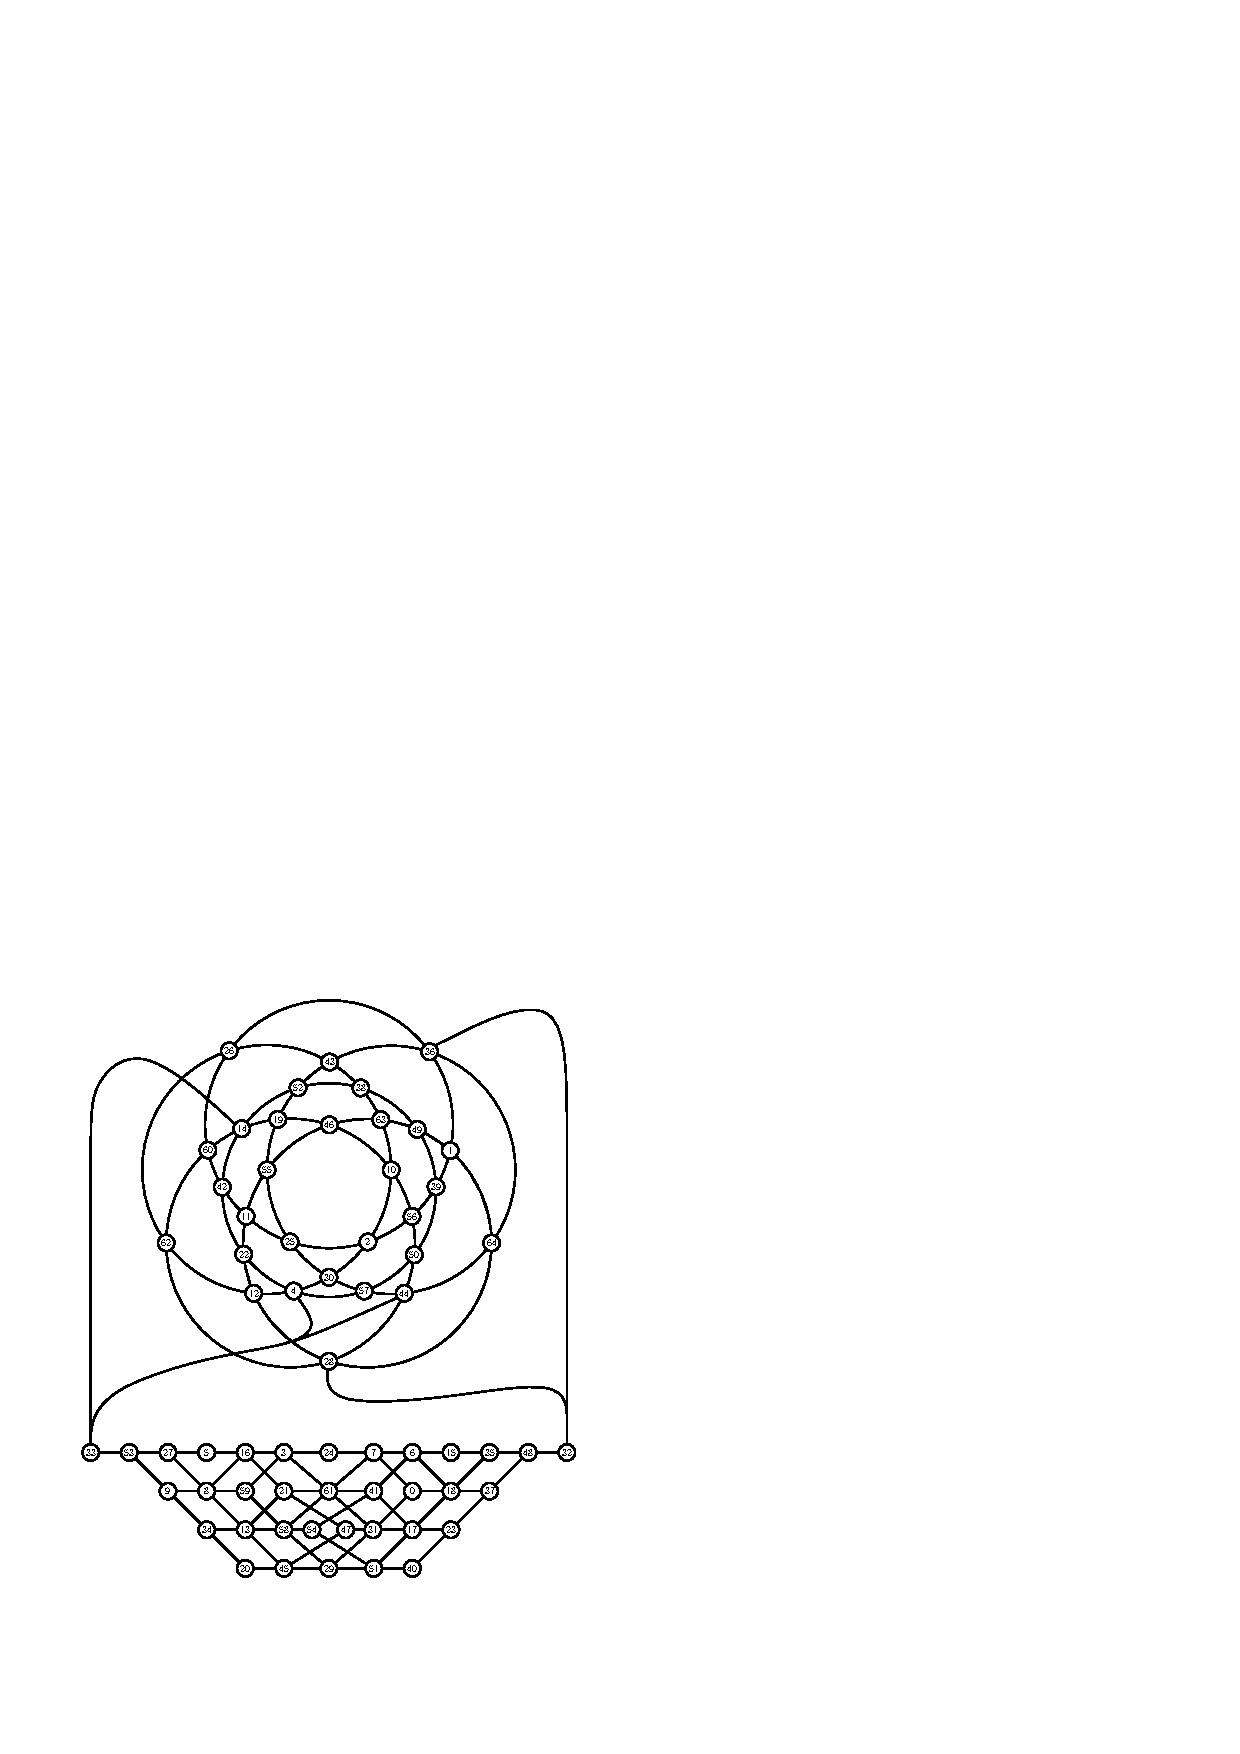
\includegraphics[scale=0.5]{example_figure}
%   \caption{A decorative flower pot, drawn by Günter Rote.}
%   \label{fig:example}
% \end{figure}

% \begin{table}[t]
%   \caption{Summary of our results.}
%   \label{tab:table}
%   \begin{tabular}{cc}
%     This & is\\
%     a & table
%   \end{tabular}
% \end{table}

% There should be some more text explaining
% research results---summarized in Table~\ref{tab:table}---in some additional sections,
% but since this is only an example file \dots

% An enumeration:
% \begin{itemize}
% \item a
% \begin{itemize}
%   \item 0
%   \item 1
% \end{itemize}
% \item b
% \end{itemize}

% \begin{lemma}
%   % Some mathematics, not entirely convincing.
%   The following formula holds
%   for all integers $n>0$\textup:
% \begin{equation}
%   \label{eq:sum-formula}
%   \sum_{i=1}^{n} i = \frac{n(n+1)}{2}
% \end{equation}
% \end{lemma}
% \begin{proof} (Not entirely convincing)
% Let \(T(n) := \frac{n(n+1)}{2}\) denote the claimed formula.
% \begin{align}
%   T(n) - T(n-1) &= \frac{n(n+1)}{2} - \frac{(n-1)n}{2}
% \nonumber
%   \\
%                 &= \frac{n(n+1) - (n-1)n}{2}
% \nonumber
%   \\
%                 &= \frac{n^2+n - (n^2+n)}{2} = \frac {2n}{2} = n
% \label{eq:diff}
% \end{align}
% The induction basis $T(0)=\frac{0\cdot 1}2 = 0$, together with~\eqref{eq:diff},
% establishes~\eqref{eq:sum-formula}.
% \end{proof}

% \begin{lemma}
%   And then we also found this lemma, which we state without proof.
%   \qed
% \end{lemma}

% \section{Conclusion}

% What we did is amazing and improves everything that was there before,
% in particular when compared to~\cite{g-atpwog-2006}.



% \subparagraph*{Acknowledgments.} We thank the organizers for
% the tasty cookies.

% \appendix

% \vspace{0.5cm}

% \noindent {\bf This is for an appendix in case you need it}

% \section{First section of the appendix}

% \subsection{A first subsection}

% \begin{theorem}
% How are you?
% \end{theorem}

% \begin{theorem}
% Fine, and how are you?
% \end{theorem}

% \subsection{A second subsection}

% \begin{theorem}
% Is this a true theorem?
% \end{theorem}

% \begin{theorem}
% This is not a theorem.
% \end{theorem}

% \section{Second section of the appendix}

% \subsection{A first subsection of the second section}

% \begin{theorem}
% Is this a formal proposition?
% \end{theorem}

% \begin{theorem}
% No, it is not.
% \end{theorem}

% \subsection{A second subsection of the second section}

% \begin{theorem}
% EuroCG is a nice workshop.
% \end{theorem}

% \begin{theorem}
% Yes, it is.
% \end{theorem}

\clearpage 

\bibliography{references}

\end{document}
